\documentclass[]{book}
\usepackage{lmodern}
\usepackage{amssymb,amsmath}
\usepackage{ifxetex,ifluatex}
\usepackage{fixltx2e} % provides \textsubscript
\ifnum 0\ifxetex 1\fi\ifluatex 1\fi=0 % if pdftex
  \usepackage[T1]{fontenc}
  \usepackage[utf8]{inputenc}
\else % if luatex or xelatex
  \ifxetex
    \usepackage{mathspec}
  \else
    \usepackage{fontspec}
  \fi
  \defaultfontfeatures{Ligatures=TeX,Scale=MatchLowercase}
\fi
% use upquote if available, for straight quotes in verbatim environments
\IfFileExists{upquote.sty}{\usepackage{upquote}}{}
% use microtype if available
\IfFileExists{microtype.sty}{%
\usepackage{microtype}
\UseMicrotypeSet[protrusion]{basicmath} % disable protrusion for tt fonts
}{}
\usepackage[margin=1in]{geometry}
\usepackage{hyperref}
\hypersetup{unicode=true,
            pdftitle={R for Psych Handbook},
            pdfauthor={David John Baker},
            pdfborder={0 0 0},
            breaklinks=true}
\urlstyle{same}  % don't use monospace font for urls
\usepackage{natbib}
\bibliographystyle{apalike}
\usepackage{color}
\usepackage{fancyvrb}
\newcommand{\VerbBar}{|}
\newcommand{\VERB}{\Verb[commandchars=\\\{\}]}
\DefineVerbatimEnvironment{Highlighting}{Verbatim}{commandchars=\\\{\}}
% Add ',fontsize=\small' for more characters per line
\usepackage{framed}
\definecolor{shadecolor}{RGB}{248,248,248}
\newenvironment{Shaded}{\begin{snugshade}}{\end{snugshade}}
\newcommand{\KeywordTok}[1]{\textcolor[rgb]{0.13,0.29,0.53}{\textbf{#1}}}
\newcommand{\DataTypeTok}[1]{\textcolor[rgb]{0.13,0.29,0.53}{#1}}
\newcommand{\DecValTok}[1]{\textcolor[rgb]{0.00,0.00,0.81}{#1}}
\newcommand{\BaseNTok}[1]{\textcolor[rgb]{0.00,0.00,0.81}{#1}}
\newcommand{\FloatTok}[1]{\textcolor[rgb]{0.00,0.00,0.81}{#1}}
\newcommand{\ConstantTok}[1]{\textcolor[rgb]{0.00,0.00,0.00}{#1}}
\newcommand{\CharTok}[1]{\textcolor[rgb]{0.31,0.60,0.02}{#1}}
\newcommand{\SpecialCharTok}[1]{\textcolor[rgb]{0.00,0.00,0.00}{#1}}
\newcommand{\StringTok}[1]{\textcolor[rgb]{0.31,0.60,0.02}{#1}}
\newcommand{\VerbatimStringTok}[1]{\textcolor[rgb]{0.31,0.60,0.02}{#1}}
\newcommand{\SpecialStringTok}[1]{\textcolor[rgb]{0.31,0.60,0.02}{#1}}
\newcommand{\ImportTok}[1]{#1}
\newcommand{\CommentTok}[1]{\textcolor[rgb]{0.56,0.35,0.01}{\textit{#1}}}
\newcommand{\DocumentationTok}[1]{\textcolor[rgb]{0.56,0.35,0.01}{\textbf{\textit{#1}}}}
\newcommand{\AnnotationTok}[1]{\textcolor[rgb]{0.56,0.35,0.01}{\textbf{\textit{#1}}}}
\newcommand{\CommentVarTok}[1]{\textcolor[rgb]{0.56,0.35,0.01}{\textbf{\textit{#1}}}}
\newcommand{\OtherTok}[1]{\textcolor[rgb]{0.56,0.35,0.01}{#1}}
\newcommand{\FunctionTok}[1]{\textcolor[rgb]{0.00,0.00,0.00}{#1}}
\newcommand{\VariableTok}[1]{\textcolor[rgb]{0.00,0.00,0.00}{#1}}
\newcommand{\ControlFlowTok}[1]{\textcolor[rgb]{0.13,0.29,0.53}{\textbf{#1}}}
\newcommand{\OperatorTok}[1]{\textcolor[rgb]{0.81,0.36,0.00}{\textbf{#1}}}
\newcommand{\BuiltInTok}[1]{#1}
\newcommand{\ExtensionTok}[1]{#1}
\newcommand{\PreprocessorTok}[1]{\textcolor[rgb]{0.56,0.35,0.01}{\textit{#1}}}
\newcommand{\AttributeTok}[1]{\textcolor[rgb]{0.77,0.63,0.00}{#1}}
\newcommand{\RegionMarkerTok}[1]{#1}
\newcommand{\InformationTok}[1]{\textcolor[rgb]{0.56,0.35,0.01}{\textbf{\textit{#1}}}}
\newcommand{\WarningTok}[1]{\textcolor[rgb]{0.56,0.35,0.01}{\textbf{\textit{#1}}}}
\newcommand{\AlertTok}[1]{\textcolor[rgb]{0.94,0.16,0.16}{#1}}
\newcommand{\ErrorTok}[1]{\textcolor[rgb]{0.64,0.00,0.00}{\textbf{#1}}}
\newcommand{\NormalTok}[1]{#1}
\usepackage{longtable,booktabs}
\usepackage{graphicx,grffile}
\makeatletter
\def\maxwidth{\ifdim\Gin@nat@width>\linewidth\linewidth\else\Gin@nat@width\fi}
\def\maxheight{\ifdim\Gin@nat@height>\textheight\textheight\else\Gin@nat@height\fi}
\makeatother
% Scale images if necessary, so that they will not overflow the page
% margins by default, and it is still possible to overwrite the defaults
% using explicit options in \includegraphics[width, height, ...]{}
\setkeys{Gin}{width=\maxwidth,height=\maxheight,keepaspectratio}
\IfFileExists{parskip.sty}{%
\usepackage{parskip}
}{% else
\setlength{\parindent}{0pt}
\setlength{\parskip}{6pt plus 2pt minus 1pt}
}
\setlength{\emergencystretch}{3em}  % prevent overfull lines
\providecommand{\tightlist}{%
  \setlength{\itemsep}{0pt}\setlength{\parskip}{0pt}}
\setcounter{secnumdepth}{5}
% Redefines (sub)paragraphs to behave more like sections
\ifx\paragraph\undefined\else
\let\oldparagraph\paragraph
\renewcommand{\paragraph}[1]{\oldparagraph{#1}\mbox{}}
\fi
\ifx\subparagraph\undefined\else
\let\oldsubparagraph\subparagraph
\renewcommand{\subparagraph}[1]{\oldsubparagraph{#1}\mbox{}}
\fi

%%% Use protect on footnotes to avoid problems with footnotes in titles
\let\rmarkdownfootnote\footnote%
\def\footnote{\protect\rmarkdownfootnote}

%%% Change title format to be more compact
\usepackage{titling}

% Create subtitle command for use in maketitle
\newcommand{\subtitle}[1]{
  \posttitle{
    \begin{center}\large#1\end{center}
    }
}

\setlength{\droptitle}{-2em}
  \title{R for Psych Handbook}
  \pretitle{\vspace{\droptitle}\centering\huge}
  \posttitle{\par}
  \author{David John Baker}
  \preauthor{\centering\large\emph}
  \postauthor{\par}
  \predate{\centering\large\emph}
  \postdate{\par}
  \date{2018-04-09}

\usepackage{booktabs}
\usepackage{amsthm}
\makeatletter
\def\thm@space@setup{%
  \thm@preskip=8pt plus 2pt minus 4pt
  \thm@postskip=\thm@preskip
}
\makeatother

\usepackage{amsthm}
\newtheorem{theorem}{Theorem}[chapter]
\newtheorem{lemma}{Lemma}[chapter]
\theoremstyle{definition}
\newtheorem{definition}{Definition}[chapter]
\newtheorem{corollary}{Corollary}[chapter]
\newtheorem{proposition}{Proposition}[chapter]
\theoremstyle{definition}
\newtheorem{example}{Example}[chapter]
\theoremstyle{definition}
\newtheorem{exercise}{Exercise}[chapter]
\theoremstyle{remark}
\newtheorem*{remark}{Remark}
\newtheorem*{solution}{Solution}
\begin{document}
\maketitle

{
\setcounter{tocdepth}{1}
\tableofcontents
}
\chapter{Preface}\label{preface}

This book serves as a collection of resources used in the LSU
psychological statistics courses. It contains some lecture notes, as
well as R code and data to run each of the examples in R.

The book is still under construction and if you would like to help out
with it, please get in touch!

The majority of the content comes from having taken and then TA's for
the LSU psychology department's stats courses. Was given oppertunity to
work for psych department as music student, partially because of R, and
writing this handbook was way of saying thank you for the great
experience that I had. Content was generated by both Jason Hicks and
Jason Harman, I just provided R as the glue to hold it all together.
Idea is that anyone going through the LSU stats rotation would be able
to if they wanted put in the extra work and learn R while they are doing
the assigments in SPSS. Data and content are from previous years, form
same, content different.

As noted in next chapter, it's hard to learn R, but worth doing it.
Personally found that R has opened up more oppertunities than anything
else I have invested in. See it as investing in self. Got started with
it because of guy who advised my Masters thesis. If you feel like you
can't do this, know that reason I started R is I knew so little about
computers, Daniel had to show me how to do an IFELSE() statement in
Excel. At that point figured if I was going to learn, might as well be
frustrated and get a better product out of it.

One thing to learn a lot by running these examples, though the best way
forward is to find your own dataset and start to set up project with it.

Beauty of R is that you are trying to become a researcher. R is
cullinary school of statistics. SPSS is a microwave. Saw that on
twitter.

Let's get cooking.

\chapter{Introduction to R}\label{intro}

Before starting out, it's worth mentioning that R has a steep learning
curve compared to other statistical softwares. While there are tons of
blog posts as to why you should learn R, I will keep my list quick so if
you get discouraged at any point, you can come back to this list and get
reinspired before R starts paying you back.

\begin{enumerate}
\def\labelenumi{\arabic{enumi}.}
\tightlist
\item
  The R community is fantastic, check out \#rstats on Twitter (this is
  really my favorite reason)
\item
  R will always be free because the people behind it believe in open
  source principles LINK.
\item
  Time spent learning R is time spent learning how computers work, if
  you learn about R, you are also learning computer programming. Time
  spent in something like SPSS or SAS does not easily tranfer to other
  programs.
\item
  On r-jobs.com the way they decide to split jobs is jobs that make
  above and below \$100,000.
\item
  R is your ticket out of academia, if you need it.
\end{enumerate}

\section{Getting Started}\label{getting-started}

Since this book is about statistics and R, the introduction to all
things R is a bit shorter than other guides. If you need help, find a
friend (or email the author of this book) and they will get you started.
The first things you need to do is download R from CRAN, then get the
latest version of RStudio. RStudio is an IDE that makes working in R a
lot easier. Do not use R without it.

Once you have that, you can start to play around with this.

\section{Setting The Working
Directory}\label{setting-the-working-directory}

At the end a long writing session you normally have to find a place to
save that journal article you are working on. You do this by clicking
`Save As' then finding where to stick it and what to call it. If you are
programming you need to do this right away by saving your script (the
what) and setting your working directory (the where).

Once you have a new script set up, now we can start to run the next
commands. This chapter covers a few basic things

\begin{itemize}
\tightlist
\item
  The rationale behind to writing scripts and code
\item
  R as Calculator
\item
  Data Structures
\item
  Manipulating Data
\item
  Tons of functions
\item
  Whirlwind tour of R for psychologists
\end{itemize}

The goals of this chapter are to:

\begin{itemize}
\tightlist
\item
  Learn Basics of R and RStudio
\item
  Practice concepts with simple examples
\item
  Familiarize with vast array of functions
\item
  Have vocabulary and ``R'' way to think about problem solving
\end{itemize}

\section{Rationale}\label{rationale}

Easily reproducible Less Human Error in cleaning Time invested in
programming transfers Pretty Graphs Open Science Huge integration

\section{R as Calculator}\label{r-as-calculator}

The Console of R is where all the action happens. You can use it just
like you would use a calculator. Try to do some basic math operations in
it.

\begin{Shaded}
\begin{Highlighting}[]
\DecValTok{2} \OperatorTok{+}\StringTok{ }\DecValTok{2}
\end{Highlighting}
\end{Shaded}

\begin{verbatim}
## [1] 4
\end{verbatim}

\begin{Shaded}
\begin{Highlighting}[]
\DecValTok{5} \OperatorTok{-}\StringTok{ }\DecValTok{2}
\end{Highlighting}
\end{Shaded}

\begin{verbatim}
## [1] 3
\end{verbatim}

\begin{Shaded}
\begin{Highlighting}[]
\DecValTok{10} \OperatorTok{/}\StringTok{ }\DecValTok{4}
\end{Highlighting}
\end{Shaded}

\begin{verbatim}
## [1] 2.5
\end{verbatim}

\begin{Shaded}
\begin{Highlighting}[]
\DecValTok{9} \OperatorTok{*}\StringTok{ }\DecValTok{200}
\end{Highlighting}
\end{Shaded}

\begin{verbatim}
## [1] 1800
\end{verbatim}

\begin{Shaded}
\begin{Highlighting}[]
\KeywordTok{sqrt}\NormalTok{(}\DecValTok{81}\NormalTok{)}
\end{Highlighting}
\end{Shaded}

\begin{verbatim}
## [1] 9
\end{verbatim}

\begin{Shaded}
\begin{Highlighting}[]
\DecValTok{10} \OperatorTok{>}\StringTok{ }\DecValTok{4}
\end{Highlighting}
\end{Shaded}

\begin{verbatim}
## [1] TRUE
\end{verbatim}

\begin{Shaded}
\begin{Highlighting}[]
\DecValTok{2} \OperatorTok{<}\StringTok{ }\OperatorTok{-}\DecValTok{1}
\end{Highlighting}
\end{Shaded}

\begin{verbatim}
## [1] FALSE
\end{verbatim}

You don't always want to print your output and retype it in. Idea is to
be very lazy (efficient).

Save some math to an object with the \textless{}- operator, then
manipulate that.

\begin{Shaded}
\begin{Highlighting}[]
\NormalTok{foo <-}\StringTok{ }\DecValTok{2} \OperatorTok{*}\StringTok{ }\DecValTok{3}
\NormalTok{foo }\OperatorTok{*}\StringTok{ }\DecValTok{6}
\end{Highlighting}
\end{Shaded}

\begin{verbatim}
## [1] 36
\end{verbatim}

Notice what has popped up in your environment in RStudio!

Let's get more efficient.

\begin{Shaded}
\begin{Highlighting}[]
\NormalTok{yearsInGradSchool <-}\StringTok{ }\KeywordTok{c}\NormalTok{(}\DecValTok{2}\NormalTok{,}\DecValTok{1}\NormalTok{,}\DecValTok{4}\NormalTok{,}\DecValTok{5}\NormalTok{,}\DecValTok{6}\NormalTok{,}\DecValTok{7}\NormalTok{,}\DecValTok{3}\NormalTok{,}\DecValTok{2}\NormalTok{,}\DecValTok{4}\NormalTok{,}\DecValTok{5}\NormalTok{,}\DecValTok{3}\NormalTok{)}
\end{Highlighting}
\end{Shaded}

talk about the c function.

\begin{Shaded}
\begin{Highlighting}[]
\NormalTok{yearsInGradSchool }\OperatorTok{*}\StringTok{ }\DecValTok{3}
\end{Highlighting}
\end{Shaded}

\begin{verbatim}
##  [1]  6  3 12 15 18 21  9  6 12 15  9
\end{verbatim}

Or this

\begin{Shaded}
\begin{Highlighting}[]
\NormalTok{yearsInGradSchool }\OperatorTok{-}\StringTok{ }\DecValTok{2}
\end{Highlighting}
\end{Shaded}

\begin{verbatim}
##  [1]  0 -1  2  3  4  5  1  0  2  3  1
\end{verbatim}

\begin{Shaded}
\begin{Highlighting}[]
\NormalTok{yearsInGradSchool }\OperatorTok{<}\StringTok{ }\DecValTok{2}
\end{Highlighting}
\end{Shaded}

\begin{verbatim}
##  [1] FALSE  TRUE FALSE FALSE FALSE FALSE FALSE FALSE FALSE FALSE FALSE
\end{verbatim}

\begin{Shaded}
\begin{Highlighting}[]
\KeywordTok{mean}\NormalTok{(yearsInGradSchool)}
\end{Highlighting}
\end{Shaded}

\begin{verbatim}
## [1] 3.818182
\end{verbatim}

\begin{Shaded}
\begin{Highlighting}[]
\KeywordTok{sd}\NormalTok{(yearsInGradSchool)}
\end{Highlighting}
\end{Shaded}

\begin{verbatim}
## [1] 1.834022
\end{verbatim}

\begin{Shaded}
\begin{Highlighting}[]
\KeywordTok{hist}\NormalTok{(yearsInGradSchool)}
\end{Highlighting}
\end{Shaded}

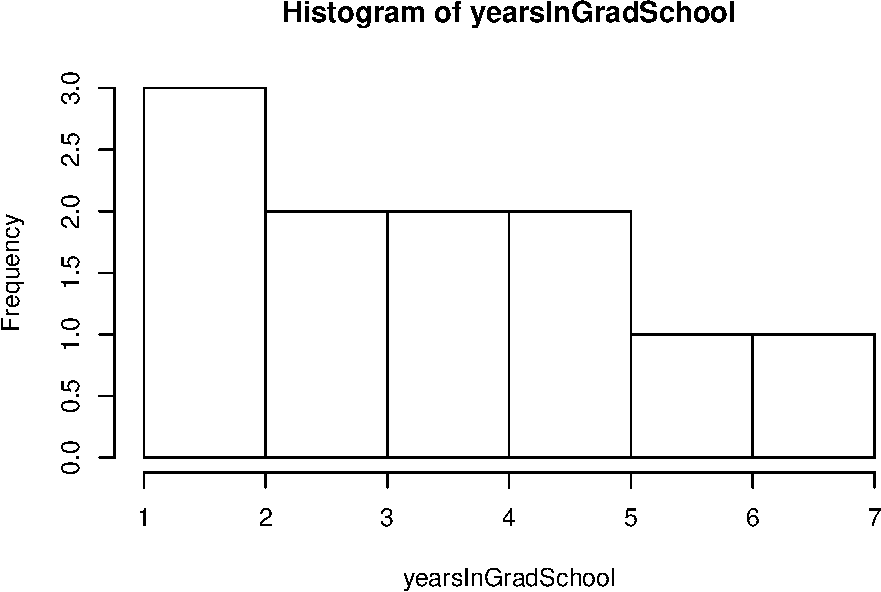
\includegraphics{bookdown-demo_files/figure-latex/unnamed-chunk-8-1.pdf}

\begin{Shaded}
\begin{Highlighting}[]
\KeywordTok{scale}\NormalTok{(yearsInGradSchool)}
\end{Highlighting}
\end{Shaded}

\begin{verbatim}
##              [,1]
##  [1,] -0.99136319
##  [2,] -1.53661295
##  [3,]  0.09913632
##  [4,]  0.64438608
##  [5,]  1.18963583
##  [6,]  1.73488559
##  [7,] -0.44611344
##  [8,] -0.99136319
##  [9,]  0.09913632
## [10,]  0.64438608
## [11,] -0.44611344
## attr(,"scaled:center")
## [1] 3.818182
## attr(,"scaled:scale")
## [1] 1.834022
\end{verbatim}

\begin{Shaded}
\begin{Highlighting}[]
\KeywordTok{range}\NormalTok{(yearsInGradSchool)}
\end{Highlighting}
\end{Shaded}

\begin{verbatim}
## [1] 1 7
\end{verbatim}

\begin{Shaded}
\begin{Highlighting}[]
\KeywordTok{min}\NormalTok{(yearsInGradSchool)}
\end{Highlighting}
\end{Shaded}

\begin{verbatim}
## [1] 1
\end{verbatim}

\begin{Shaded}
\begin{Highlighting}[]
\KeywordTok{class}\NormalTok{(yearsInGradSchool)}
\end{Highlighting}
\end{Shaded}

\begin{verbatim}
## [1] "numeric"
\end{verbatim}

\begin{Shaded}
\begin{Highlighting}[]
\KeywordTok{str}\NormalTok{(yearsInGradSchool)}
\end{Highlighting}
\end{Shaded}

\begin{verbatim}
##  num [1:11] 2 1 4 5 6 7 3 2 4 5 ...
\end{verbatim}

\begin{Shaded}
\begin{Highlighting}[]
\KeywordTok{summary}\NormalTok{(yearsInGradSchool)}
\end{Highlighting}
\end{Shaded}

\begin{verbatim}
##    Min. 1st Qu.  Median    Mean 3rd Qu.    Max. 
##   1.000   2.500   4.000   3.818   5.000   7.000
\end{verbatim}

\begin{Shaded}
\begin{Highlighting}[]
\NormalTok{yearsInGradSchool <-}\StringTok{ }\KeywordTok{c}\NormalTok{(}\DecValTok{2}\NormalTok{,}\DecValTok{1}\NormalTok{,}\DecValTok{4}\NormalTok{,}\DecValTok{5}\NormalTok{,}\DecValTok{6}\NormalTok{,}\DecValTok{7}\NormalTok{,}\DecValTok{3}\NormalTok{,}\DecValTok{2}\NormalTok{,}\DecValTok{4}\NormalTok{,}\DecValTok{5}\NormalTok{,}\DecValTok{3}\NormalTok{)}
\NormalTok{classesTaken <-}\StringTok{ }\KeywordTok{c}\NormalTok{(}\DecValTok{5}\NormalTok{,}\DecValTok{2}\NormalTok{,}\DecValTok{5}\NormalTok{,}\DecValTok{7}\NormalTok{,}\DecValTok{9}\NormalTok{,}\DecValTok{9}\NormalTok{,}\DecValTok{2}\NormalTok{,}\DecValTok{8}\NormalTok{,}\DecValTok{4}\NormalTok{,}\DecValTok{7}\NormalTok{,}\DecValTok{2}\NormalTok{)}
\NormalTok{gradData <-}\StringTok{ }\KeywordTok{data.frame}\NormalTok{(yearsInGradSchool,classesTaken)}
\end{Highlighting}
\end{Shaded}

\begin{Shaded}
\begin{Highlighting}[]
\KeywordTok{cor}\NormalTok{(yearsInGradSchool,classesTaken)}
\end{Highlighting}
\end{Shaded}

\begin{verbatim}
## [1] 0.6763509
\end{verbatim}

Basic plots, arguments. ggplot and libraries

\begin{Shaded}
\begin{Highlighting}[]
\KeywordTok{plot}\NormalTok{(yearsInGradSchool,classesTaken, }
     \DataTypeTok{data =}\NormalTok{ gradData, }
     \DataTypeTok{main =} \StringTok{"My Plot"}\NormalTok{, }
     \DataTypeTok{xlab =} \StringTok{"Years in Grad School"}\NormalTok{, }
     \DataTypeTok{ylab =} \StringTok{"Classes Taken"}\NormalTok{)}
\end{Highlighting}
\end{Shaded}

\begin{verbatim}
## Warning in plot.window(...): "data" is not a graphical parameter
\end{verbatim}

\begin{verbatim}
## Warning in plot.xy(xy, type, ...): "data" is not a graphical parameter
\end{verbatim}

\begin{verbatim}
## Warning in axis(side = side, at = at, labels = labels, ...): "data" is not
## a graphical parameter

## Warning in axis(side = side, at = at, labels = labels, ...): "data" is not
## a graphical parameter
\end{verbatim}

\begin{verbatim}
## Warning in box(...): "data" is not a graphical parameter
\end{verbatim}

\begin{verbatim}
## Warning in title(...): "data" is not a graphical parameter
\end{verbatim}

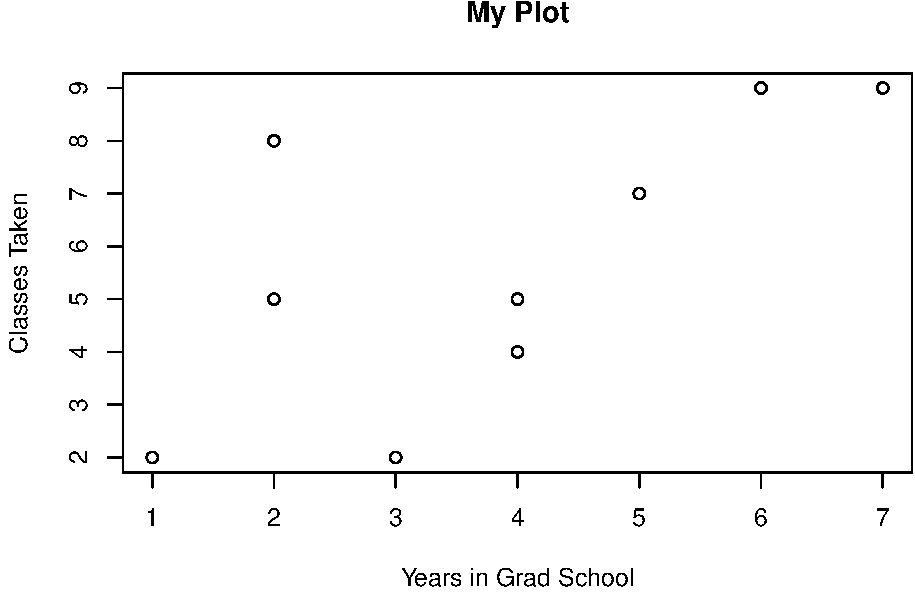
\includegraphics{bookdown-demo_files/figure-latex/unnamed-chunk-11-1.pdf}

\section{Data Exploration}\label{data-exploration}

\begin{Shaded}
\begin{Highlighting}[]
\KeywordTok{str}\NormalTok{(iris)}
\end{Highlighting}
\end{Shaded}

\begin{verbatim}
## 'data.frame':    150 obs. of  5 variables:
##  $ Sepal.Length: num  5.1 4.9 4.7 4.6 5 5.4 4.6 5 4.4 4.9 ...
##  $ Sepal.Width : num  3.5 3 3.2 3.1 3.6 3.9 3.4 3.4 2.9 3.1 ...
##  $ Petal.Length: num  1.4 1.4 1.3 1.5 1.4 1.7 1.4 1.5 1.4 1.5 ...
##  $ Petal.Width : num  0.2 0.2 0.2 0.2 0.2 0.4 0.3 0.2 0.2 0.1 ...
##  $ Species     : Factor w/ 3 levels "setosa","versicolor",..: 1 1 1 1 1 1 1 1 1 1 ...
\end{verbatim}

\begin{Shaded}
\begin{Highlighting}[]
\KeywordTok{class}\NormalTok{(iris)}
\end{Highlighting}
\end{Shaded}

\begin{verbatim}
## [1] "data.frame"
\end{verbatim}

\begin{Shaded}
\begin{Highlighting}[]
\KeywordTok{summary}\NormalTok{(iris)}
\end{Highlighting}
\end{Shaded}

\begin{verbatim}
##   Sepal.Length    Sepal.Width     Petal.Length    Petal.Width   
##  Min.   :4.300   Min.   :2.000   Min.   :1.000   Min.   :0.100  
##  1st Qu.:5.100   1st Qu.:2.800   1st Qu.:1.600   1st Qu.:0.300  
##  Median :5.800   Median :3.000   Median :4.350   Median :1.300  
##  Mean   :5.843   Mean   :3.057   Mean   :3.758   Mean   :1.199  
##  3rd Qu.:6.400   3rd Qu.:3.300   3rd Qu.:5.100   3rd Qu.:1.800  
##  Max.   :7.900   Max.   :4.400   Max.   :6.900   Max.   :2.500  
##        Species  
##  setosa    :50  
##  versicolor:50  
##  virginica :50  
##                 
##                 
## 
\end{verbatim}

Accessing individual `columns' is done with the \$ operator

\begin{Shaded}
\begin{Highlighting}[]
\NormalTok{iris}\OperatorTok{$}\NormalTok{Sepal.Length}
\end{Highlighting}
\end{Shaded}

\begin{verbatim}
##   [1] 5.1 4.9 4.7 4.6 5.0 5.4 4.6 5.0 4.4 4.9 5.4 4.8 4.8 4.3 5.8 5.7 5.4
##  [18] 5.1 5.7 5.1 5.4 5.1 4.6 5.1 4.8 5.0 5.0 5.2 5.2 4.7 4.8 5.4 5.2 5.5
##  [35] 4.9 5.0 5.5 4.9 4.4 5.1 5.0 4.5 4.4 5.0 5.1 4.8 5.1 4.6 5.3 5.0 7.0
##  [52] 6.4 6.9 5.5 6.5 5.7 6.3 4.9 6.6 5.2 5.0 5.9 6.0 6.1 5.6 6.7 5.6 5.8
##  [69] 6.2 5.6 5.9 6.1 6.3 6.1 6.4 6.6 6.8 6.7 6.0 5.7 5.5 5.5 5.8 6.0 5.4
##  [86] 6.0 6.7 6.3 5.6 5.5 5.5 6.1 5.8 5.0 5.6 5.7 5.7 6.2 5.1 5.7 6.3 5.8
## [103] 7.1 6.3 6.5 7.6 4.9 7.3 6.7 7.2 6.5 6.4 6.8 5.7 5.8 6.4 6.5 7.7 7.7
## [120] 6.0 6.9 5.6 7.7 6.3 6.7 7.2 6.2 6.1 6.4 7.2 7.4 7.9 6.4 6.3 6.1 7.7
## [137] 6.3 6.4 6.0 6.9 6.7 6.9 5.8 6.8 6.7 6.7 6.3 6.5 6.2 5.9
\end{verbatim}

Can you use this to plot the different numeric values against each
other?

What would the follow commands do?

\begin{Shaded}
\begin{Highlighting}[]
\KeywordTok{hist}\NormalTok{(}\KeywordTok{scale}\NormalTok{(iris}\OperatorTok{$}\NormalTok{Sepal.Length))}
\end{Highlighting}
\end{Shaded}

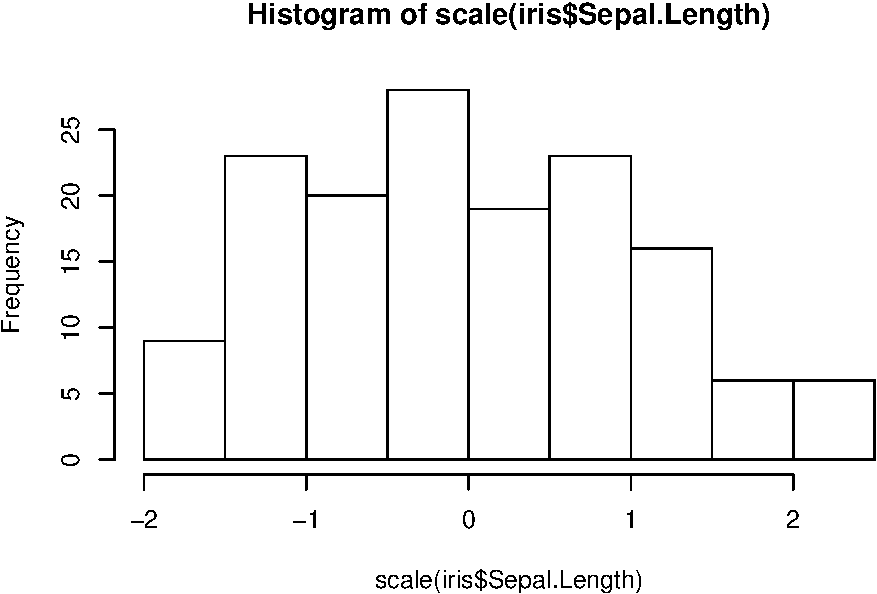
\includegraphics{bookdown-demo_files/figure-latex/unnamed-chunk-14-1.pdf}

\begin{Shaded}
\begin{Highlighting}[]
\NormalTok{iris}\OperatorTok{$}\NormalTok{Sepal.Length.scale <-}\StringTok{ }\KeywordTok{scale}\NormalTok{(iris}\OperatorTok{$}\NormalTok{Sepal.Length)}
\end{Highlighting}
\end{Shaded}

\section{Indexing}\label{indexing}

Let's combine logical indexing with creating new objects.

What do the follow commands do? Why?

\begin{Shaded}
\begin{Highlighting}[]
\NormalTok{iris[}\DecValTok{1}\NormalTok{,}\DecValTok{1}\NormalTok{]}
\end{Highlighting}
\end{Shaded}

\begin{verbatim}
## [1] 5.1
\end{verbatim}

\begin{Shaded}
\begin{Highlighting}[]
\NormalTok{iris[}\DecValTok{2}\NormalTok{,]}
\end{Highlighting}
\end{Shaded}

\begin{verbatim}
##   Sepal.Length Sepal.Width Petal.Length Petal.Width Species
## 2          4.9           3          1.4         0.2  setosa
##   Sepal.Length.scale
## 2            -1.1392
\end{verbatim}

\begin{Shaded}
\begin{Highlighting}[]
\NormalTok{iris[,}\DecValTok{5}\NormalTok{]}
\end{Highlighting}
\end{Shaded}

\begin{verbatim}
##   [1] setosa     setosa     setosa     setosa     setosa     setosa    
##   [7] setosa     setosa     setosa     setosa     setosa     setosa    
##  [13] setosa     setosa     setosa     setosa     setosa     setosa    
##  [19] setosa     setosa     setosa     setosa     setosa     setosa    
##  [25] setosa     setosa     setosa     setosa     setosa     setosa    
##  [31] setosa     setosa     setosa     setosa     setosa     setosa    
##  [37] setosa     setosa     setosa     setosa     setosa     setosa    
##  [43] setosa     setosa     setosa     setosa     setosa     setosa    
##  [49] setosa     setosa     versicolor versicolor versicolor versicolor
##  [55] versicolor versicolor versicolor versicolor versicolor versicolor
##  [61] versicolor versicolor versicolor versicolor versicolor versicolor
##  [67] versicolor versicolor versicolor versicolor versicolor versicolor
##  [73] versicolor versicolor versicolor versicolor versicolor versicolor
##  [79] versicolor versicolor versicolor versicolor versicolor versicolor
##  [85] versicolor versicolor versicolor versicolor versicolor versicolor
##  [91] versicolor versicolor versicolor versicolor versicolor versicolor
##  [97] versicolor versicolor versicolor versicolor virginica  virginica 
## [103] virginica  virginica  virginica  virginica  virginica  virginica 
## [109] virginica  virginica  virginica  virginica  virginica  virginica 
## [115] virginica  virginica  virginica  virginica  virginica  virginica 
## [121] virginica  virginica  virginica  virginica  virginica  virginica 
## [127] virginica  virginica  virginica  virginica  virginica  virginica 
## [133] virginica  virginica  virginica  virginica  virginica  virginica 
## [139] virginica  virginica  virginica  virginica  virginica  virginica 
## [145] virginica  virginica  virginica  virginica  virginica  virginica 
## Levels: setosa versicolor virginica
\end{verbatim}

\begin{Shaded}
\begin{Highlighting}[]
\NormalTok{iris[iris}\OperatorTok{$}\NormalTok{Sepal.Length }\OperatorTok{<}\StringTok{ }\DecValTok{5}\NormalTok{,]}
\end{Highlighting}
\end{Shaded}

\begin{verbatim}
##     Sepal.Length Sepal.Width Petal.Length Petal.Width    Species
## 2            4.9         3.0          1.4         0.2     setosa
## 3            4.7         3.2          1.3         0.2     setosa
## 4            4.6         3.1          1.5         0.2     setosa
## 7            4.6         3.4          1.4         0.3     setosa
## 9            4.4         2.9          1.4         0.2     setosa
## 10           4.9         3.1          1.5         0.1     setosa
## 12           4.8         3.4          1.6         0.2     setosa
## 13           4.8         3.0          1.4         0.1     setosa
## 14           4.3         3.0          1.1         0.1     setosa
## 23           4.6         3.6          1.0         0.2     setosa
## 25           4.8         3.4          1.9         0.2     setosa
## 30           4.7         3.2          1.6         0.2     setosa
## 31           4.8         3.1          1.6         0.2     setosa
## 35           4.9         3.1          1.5         0.2     setosa
## 38           4.9         3.6          1.4         0.1     setosa
## 39           4.4         3.0          1.3         0.2     setosa
## 42           4.5         2.3          1.3         0.3     setosa
## 43           4.4         3.2          1.3         0.2     setosa
## 46           4.8         3.0          1.4         0.3     setosa
## 48           4.6         3.2          1.4         0.2     setosa
## 58           4.9         2.4          3.3         1.0 versicolor
## 107          4.9         2.5          4.5         1.7  virginica
##     Sepal.Length.scale
## 2            -1.139200
## 3            -1.380727
## 4            -1.501490
## 7            -1.501490
## 9            -1.743017
## 10           -1.139200
## 12           -1.259964
## 13           -1.259964
## 14           -1.863780
## 23           -1.501490
## 25           -1.259964
## 30           -1.380727
## 31           -1.259964
## 35           -1.139200
## 38           -1.139200
## 39           -1.743017
## 42           -1.622254
## 43           -1.743017
## 46           -1.259964
## 48           -1.501490
## 58           -1.139200
## 107          -1.139200
\end{verbatim}

\begin{Shaded}
\begin{Highlighting}[]
\NormalTok{iris[,}\KeywordTok{c}\NormalTok{(}\DecValTok{1}\OperatorTok{:}\DecValTok{4}\NormalTok{)]}
\end{Highlighting}
\end{Shaded}

\begin{verbatim}
##     Sepal.Length Sepal.Width Petal.Length Petal.Width
## 1            5.1         3.5          1.4         0.2
## 2            4.9         3.0          1.4         0.2
## 3            4.7         3.2          1.3         0.2
## 4            4.6         3.1          1.5         0.2
## 5            5.0         3.6          1.4         0.2
## 6            5.4         3.9          1.7         0.4
## 7            4.6         3.4          1.4         0.3
## 8            5.0         3.4          1.5         0.2
## 9            4.4         2.9          1.4         0.2
## 10           4.9         3.1          1.5         0.1
## 11           5.4         3.7          1.5         0.2
## 12           4.8         3.4          1.6         0.2
## 13           4.8         3.0          1.4         0.1
## 14           4.3         3.0          1.1         0.1
## 15           5.8         4.0          1.2         0.2
## 16           5.7         4.4          1.5         0.4
## 17           5.4         3.9          1.3         0.4
## 18           5.1         3.5          1.4         0.3
## 19           5.7         3.8          1.7         0.3
## 20           5.1         3.8          1.5         0.3
## 21           5.4         3.4          1.7         0.2
## 22           5.1         3.7          1.5         0.4
## 23           4.6         3.6          1.0         0.2
## 24           5.1         3.3          1.7         0.5
## 25           4.8         3.4          1.9         0.2
## 26           5.0         3.0          1.6         0.2
## 27           5.0         3.4          1.6         0.4
## 28           5.2         3.5          1.5         0.2
## 29           5.2         3.4          1.4         0.2
## 30           4.7         3.2          1.6         0.2
## 31           4.8         3.1          1.6         0.2
## 32           5.4         3.4          1.5         0.4
## 33           5.2         4.1          1.5         0.1
## 34           5.5         4.2          1.4         0.2
## 35           4.9         3.1          1.5         0.2
## 36           5.0         3.2          1.2         0.2
## 37           5.5         3.5          1.3         0.2
## 38           4.9         3.6          1.4         0.1
## 39           4.4         3.0          1.3         0.2
## 40           5.1         3.4          1.5         0.2
## 41           5.0         3.5          1.3         0.3
## 42           4.5         2.3          1.3         0.3
## 43           4.4         3.2          1.3         0.2
## 44           5.0         3.5          1.6         0.6
## 45           5.1         3.8          1.9         0.4
## 46           4.8         3.0          1.4         0.3
## 47           5.1         3.8          1.6         0.2
## 48           4.6         3.2          1.4         0.2
## 49           5.3         3.7          1.5         0.2
## 50           5.0         3.3          1.4         0.2
## 51           7.0         3.2          4.7         1.4
## 52           6.4         3.2          4.5         1.5
## 53           6.9         3.1          4.9         1.5
## 54           5.5         2.3          4.0         1.3
## 55           6.5         2.8          4.6         1.5
## 56           5.7         2.8          4.5         1.3
## 57           6.3         3.3          4.7         1.6
## 58           4.9         2.4          3.3         1.0
## 59           6.6         2.9          4.6         1.3
## 60           5.2         2.7          3.9         1.4
## 61           5.0         2.0          3.5         1.0
## 62           5.9         3.0          4.2         1.5
## 63           6.0         2.2          4.0         1.0
## 64           6.1         2.9          4.7         1.4
## 65           5.6         2.9          3.6         1.3
## 66           6.7         3.1          4.4         1.4
## 67           5.6         3.0          4.5         1.5
## 68           5.8         2.7          4.1         1.0
## 69           6.2         2.2          4.5         1.5
## 70           5.6         2.5          3.9         1.1
## 71           5.9         3.2          4.8         1.8
## 72           6.1         2.8          4.0         1.3
## 73           6.3         2.5          4.9         1.5
## 74           6.1         2.8          4.7         1.2
## 75           6.4         2.9          4.3         1.3
## 76           6.6         3.0          4.4         1.4
## 77           6.8         2.8          4.8         1.4
## 78           6.7         3.0          5.0         1.7
## 79           6.0         2.9          4.5         1.5
## 80           5.7         2.6          3.5         1.0
## 81           5.5         2.4          3.8         1.1
## 82           5.5         2.4          3.7         1.0
## 83           5.8         2.7          3.9         1.2
## 84           6.0         2.7          5.1         1.6
## 85           5.4         3.0          4.5         1.5
## 86           6.0         3.4          4.5         1.6
## 87           6.7         3.1          4.7         1.5
## 88           6.3         2.3          4.4         1.3
## 89           5.6         3.0          4.1         1.3
## 90           5.5         2.5          4.0         1.3
## 91           5.5         2.6          4.4         1.2
## 92           6.1         3.0          4.6         1.4
## 93           5.8         2.6          4.0         1.2
## 94           5.0         2.3          3.3         1.0
## 95           5.6         2.7          4.2         1.3
## 96           5.7         3.0          4.2         1.2
## 97           5.7         2.9          4.2         1.3
## 98           6.2         2.9          4.3         1.3
## 99           5.1         2.5          3.0         1.1
## 100          5.7         2.8          4.1         1.3
## 101          6.3         3.3          6.0         2.5
## 102          5.8         2.7          5.1         1.9
## 103          7.1         3.0          5.9         2.1
## 104          6.3         2.9          5.6         1.8
## 105          6.5         3.0          5.8         2.2
## 106          7.6         3.0          6.6         2.1
## 107          4.9         2.5          4.5         1.7
## 108          7.3         2.9          6.3         1.8
## 109          6.7         2.5          5.8         1.8
## 110          7.2         3.6          6.1         2.5
## 111          6.5         3.2          5.1         2.0
## 112          6.4         2.7          5.3         1.9
## 113          6.8         3.0          5.5         2.1
## 114          5.7         2.5          5.0         2.0
## 115          5.8         2.8          5.1         2.4
## 116          6.4         3.2          5.3         2.3
## 117          6.5         3.0          5.5         1.8
## 118          7.7         3.8          6.7         2.2
## 119          7.7         2.6          6.9         2.3
## 120          6.0         2.2          5.0         1.5
## 121          6.9         3.2          5.7         2.3
## 122          5.6         2.8          4.9         2.0
## 123          7.7         2.8          6.7         2.0
## 124          6.3         2.7          4.9         1.8
## 125          6.7         3.3          5.7         2.1
## 126          7.2         3.2          6.0         1.8
## 127          6.2         2.8          4.8         1.8
## 128          6.1         3.0          4.9         1.8
## 129          6.4         2.8          5.6         2.1
## 130          7.2         3.0          5.8         1.6
## 131          7.4         2.8          6.1         1.9
## 132          7.9         3.8          6.4         2.0
## 133          6.4         2.8          5.6         2.2
## 134          6.3         2.8          5.1         1.5
## 135          6.1         2.6          5.6         1.4
## 136          7.7         3.0          6.1         2.3
## 137          6.3         3.4          5.6         2.4
## 138          6.4         3.1          5.5         1.8
## 139          6.0         3.0          4.8         1.8
## 140          6.9         3.1          5.4         2.1
## 141          6.7         3.1          5.6         2.4
## 142          6.9         3.1          5.1         2.3
## 143          5.8         2.7          5.1         1.9
## 144          6.8         3.2          5.9         2.3
## 145          6.7         3.3          5.7         2.5
## 146          6.7         3.0          5.2         2.3
## 147          6.3         2.5          5.0         1.9
## 148          6.5         3.0          5.2         2.0
## 149          6.2         3.4          5.4         2.3
## 150          5.9         3.0          5.1         1.8
\end{verbatim}

\begin{Shaded}
\begin{Highlighting}[]
\NormalTok{iris[}\KeywordTok{c}\NormalTok{(}\DecValTok{1}\NormalTok{,}\DecValTok{2}\NormalTok{,}\DecValTok{3}\NormalTok{,}\DecValTok{4}\NormalTok{,}\DecValTok{5}\NormalTok{,}\DecValTok{6}\NormalTok{,}\DecValTok{8}\NormalTok{),}\KeywordTok{c}\NormalTok{(}\DecValTok{1}\OperatorTok{:}\DecValTok{3}\NormalTok{,}\DecValTok{5}\NormalTok{)]}
\end{Highlighting}
\end{Shaded}

\begin{verbatim}
##   Sepal.Length Sepal.Width Petal.Length Species
## 1          5.1         3.5          1.4  setosa
## 2          4.9         3.0          1.4  setosa
## 3          4.7         3.2          1.3  setosa
## 4          4.6         3.1          1.5  setosa
## 5          5.0         3.6          1.4  setosa
## 6          5.4         3.9          1.7  setosa
## 8          5.0         3.4          1.5  setosa
\end{verbatim}

\begin{Shaded}
\begin{Highlighting}[]
\NormalTok{Setosas <-}\StringTok{ }\NormalTok{iris[iris}\OperatorTok{$}\NormalTok{Species }\OperatorTok{==}\StringTok{ "setosa"}\NormalTok{,]}
\end{Highlighting}
\end{Shaded}

This could be an entire lecture by itself!!!

\section{Whirlwind Tour of R}\label{whirlwind-tour-of-r}

R's power comes in the fact that you download packages to put on top of
base R

\begin{itemize}
\tightlist
\item
  Turning Data tables into already formatted APA Latex Tables
  (stargazer, xtable)
\item
  Creating Publication Quality Graphs (ggplot2)
\item
  Text manipulation (stringr)
\item
  Exploring data and not making chart after chart after chart (psych)
\item
  Every statistical test you could want (psych, cars, ezanova, lavaan)
\item
  Software to plot not so normal output (SEMplots)
\item
  Making Websites in R
\item
  These slides were written in R
\item
  Quickly processing huge datasets (data.table, dplyr)
\item
  Tons of Machine Learning
\end{itemize}

\begin{Shaded}
\begin{Highlighting}[]
\KeywordTok{library}\NormalTok{(ggplot2)}
\KeywordTok{ggplot}\NormalTok{(iris, }\KeywordTok{aes}\NormalTok{(}\DataTypeTok{x =}\NormalTok{ Sepal.Length, }\DataTypeTok{y =}\NormalTok{ Sepal.Width, }
                 \DataTypeTok{color =}\NormalTok{ Species), }
       \DataTypeTok{xlab =} \StringTok{"Sepal Length"}\NormalTok{,}
       \DataTypeTok{ylab =} \StringTok{"Sepal Width"}\NormalTok{,}
       \DataTypeTok{main =} \StringTok{"My Plot"}\NormalTok{) }\OperatorTok{+}\StringTok{ }\KeywordTok{geom_point}\NormalTok{()}
\end{Highlighting}
\end{Shaded}

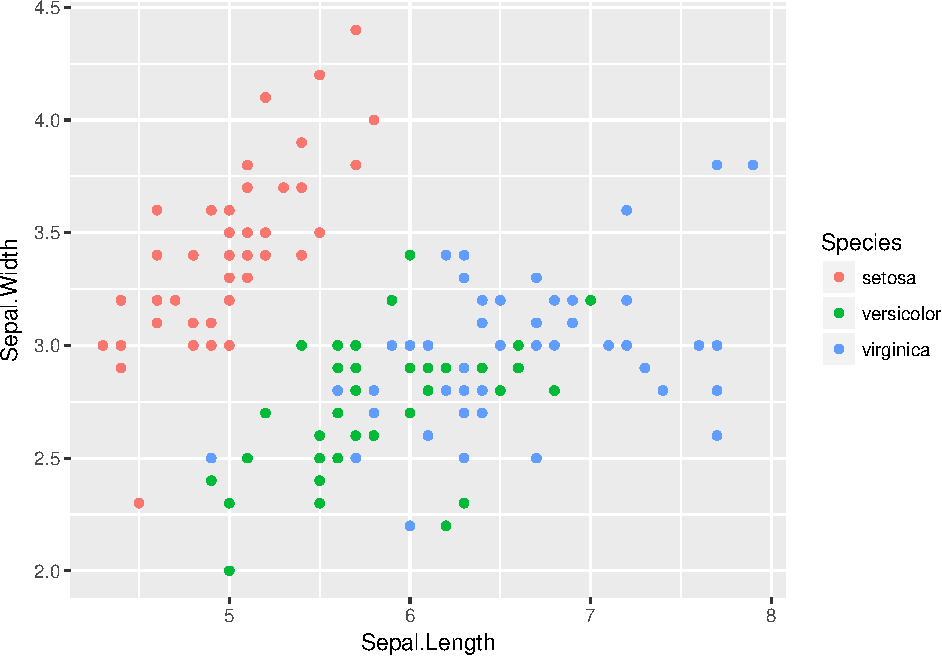
\includegraphics{bookdown-demo_files/figure-latex/unnamed-chunk-16-1.pdf}

Or stuff for data exploration

\begin{Shaded}
\begin{Highlighting}[]
\KeywordTok{library}\NormalTok{(psych)}
\end{Highlighting}
\end{Shaded}

\begin{verbatim}
## 
## Attaching package: 'psych'
\end{verbatim}

\begin{verbatim}
## The following objects are masked from 'package:ggplot2':
## 
##     %+%, alpha
\end{verbatim}

\begin{Shaded}
\begin{Highlighting}[]
\KeywordTok{pairs.panels}\NormalTok{(iris)}
\end{Highlighting}
\end{Shaded}

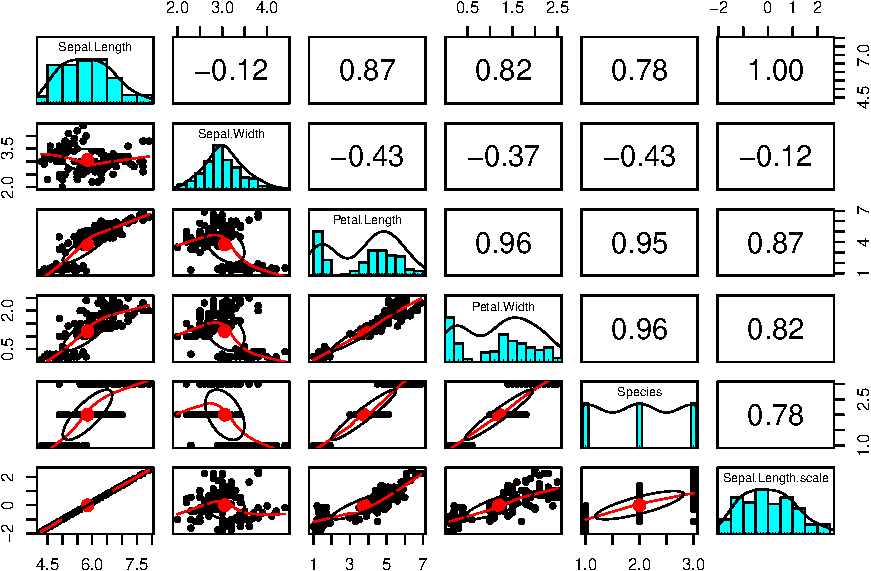
\includegraphics{bookdown-demo_files/figure-latex/unnamed-chunk-17-1.pdf}

\section{Functions for Psychologists}\label{functions-for-psychologists}

\begin{itemize}
\tightlist
\item
  nlme() and lme4() for Multilevel Modeling
\item
  lavaan() for Latent Variable Analysis
\item
  ezAnova() for ANOVA based testing; the anova() function does model
  comparisons
\item
  profileR for Repeated Measures MANOVA
\item
  glm() and lm() for linear models
\item
  caret() for Machine Learning
\end{itemize}

\section{Resources}\label{resources}

LINK THESE IN

\begin{itemize}
\tightlist
\item
  swirl
\item
  stackoverflow.com
\item
  Twitter
\item
  Your peers
\item
  R Community is fantastic (tidyverse!!!)
\end{itemize}

\subsection{Template Stuff}\label{template-stuff}

You can label chapter and section titles using \texttt{\{\#label\}}
after them, e.g., we can reference Chapter \ref{intro}. If you do not
manually label them, there will be automatic labels anyway, e.g.,
Chapter \ref{methods}.

Figures and tables with captions will be placed in \texttt{figure} and
\texttt{table} environments, respectively.

\begin{Shaded}
\begin{Highlighting}[]
\KeywordTok{par}\NormalTok{(}\DataTypeTok{mar =} \KeywordTok{c}\NormalTok{(}\DecValTok{4}\NormalTok{, }\DecValTok{4}\NormalTok{, .}\DecValTok{1}\NormalTok{, .}\DecValTok{1}\NormalTok{))}
\KeywordTok{plot}\NormalTok{(pressure, }\DataTypeTok{type =} \StringTok{'b'}\NormalTok{, }\DataTypeTok{pch =} \DecValTok{19}\NormalTok{)}
\end{Highlighting}
\end{Shaded}

\begin{figure}

{\centering 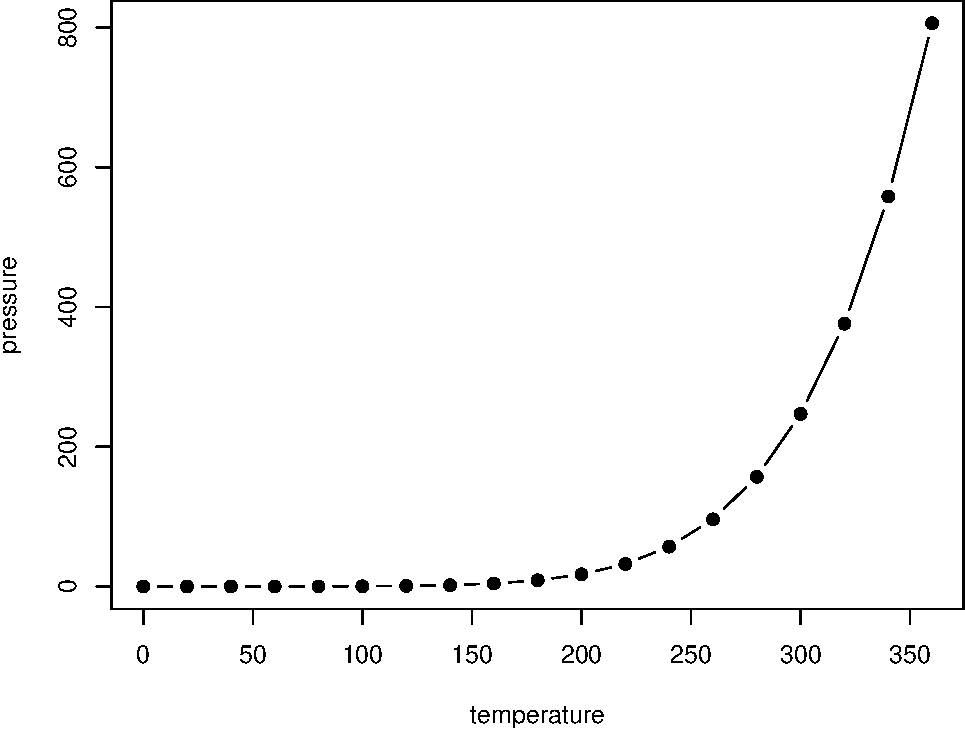
\includegraphics[width=0.8\linewidth]{bookdown-demo_files/figure-latex/nice-fig-1} 

}

\caption{Here is a nice figure!}\label{fig:nice-fig}
\end{figure}

Reference a figure by its code chunk label with the \texttt{fig:}
prefix, e.g., see Figure \ref{fig:nice-fig}. Similarly, you can
reference tables generated from \texttt{knitr::kable()}, e.g., see Table
\ref{tab:nice-tab}.

\begin{Shaded}
\begin{Highlighting}[]
\NormalTok{knitr}\OperatorTok{::}\KeywordTok{kable}\NormalTok{(}
  \KeywordTok{head}\NormalTok{(iris, }\DecValTok{20}\NormalTok{), }\DataTypeTok{caption =} \StringTok{'Here is a nice table!'}\NormalTok{,}
  \DataTypeTok{booktabs =} \OtherTok{TRUE}
\NormalTok{)}
\end{Highlighting}
\end{Shaded}

\begin{table}

\caption{\label{tab:nice-tab}Here is a nice table!}
\centering
\begin{tabular}[t]{rrrrlr}
\toprule
Sepal.Length & Sepal.Width & Petal.Length & Petal.Width & Species & Sepal.Length.scale\\
\midrule
5.1 & 3.5 & 1.4 & 0.2 & setosa & -0.89767388\\
4.9 & 3.0 & 1.4 & 0.2 & setosa & -1.13920048\\
4.7 & 3.2 & 1.3 & 0.2 & setosa & -1.38072709\\
4.6 & 3.1 & 1.5 & 0.2 & setosa & -1.50149039\\
5.0 & 3.6 & 1.4 & 0.2 & setosa & -1.01843718\\
\addlinespace
5.4 & 3.9 & 1.7 & 0.4 & setosa & -0.53538397\\
4.6 & 3.4 & 1.4 & 0.3 & setosa & -1.50149039\\
5.0 & 3.4 & 1.5 & 0.2 & setosa & -1.01843718\\
4.4 & 2.9 & 1.4 & 0.2 & setosa & -1.74301699\\
4.9 & 3.1 & 1.5 & 0.1 & setosa & -1.13920048\\
\addlinespace
5.4 & 3.7 & 1.5 & 0.2 & setosa & -0.53538397\\
4.8 & 3.4 & 1.6 & 0.2 & setosa & -1.25996379\\
4.8 & 3.0 & 1.4 & 0.1 & setosa & -1.25996379\\
4.3 & 3.0 & 1.1 & 0.1 & setosa & -1.86378030\\
5.8 & 4.0 & 1.2 & 0.2 & setosa & -0.05233076\\
\addlinespace
5.7 & 4.4 & 1.5 & 0.4 & setosa & -0.17309407\\
5.4 & 3.9 & 1.3 & 0.4 & setosa & -0.53538397\\
5.1 & 3.5 & 1.4 & 0.3 & setosa & -0.89767388\\
5.7 & 3.8 & 1.7 & 0.3 & setosa & -0.17309407\\
5.1 & 3.8 & 1.5 & 0.3 & setosa & -0.89767388\\
\bottomrule
\end{tabular}
\end{table}

You can write citations, too. For example, we are using the
\textbf{bookdown} package \citep{R-bookdown} in this sample book, which
was built on top of R Markdown and \textbf{knitr} \citep{xie2015}.

\chapter{Data Manipulation in R}\label{data-manipulation-in-r}

\begin{Shaded}
\begin{Highlighting}[]
\CommentTok{# #======================================================================================================}
\CommentTok{# # LSUserRs Data Cleaning Template (Title Your Script)}
\CommentTok{# # Say a couple of the things that it does here. Who wrote it?}
\CommentTok{# # When was the last edit? What does it do? Does it work with any data type?}
\CommentTok{# # Rubber duck this as much as possible because you won't remember}
\CommentTok{# # what you did in 6 months. Especially if you come up with something clever.}
\CommentTok{# #======================================================================================================}
\CommentTok{# # TRY YOUR BEST TO NOT JUST COPY AND PASTE CODE, GOOGLE WHAT YOU WANT, GET FAMILIAR WITH A FUNCTION'S}
\CommentTok{# # ARGUMENTS AND EMBRACE YOUR INNER NERD AND READ THE DOCUMENTATION!! }
\CommentTok{# #======================================================================================================}
\CommentTok{# # Import Libraries }
\CommentTok{# #--------------------------------------------------}
\CommentTok{# # Load all libraries at the start of your script, remember they have to be installed first! }
\CommentTok{# library(stringr)}
\CommentTok{# library(data.table)}
\CommentTok{# library(psych)}
\CommentTok{# }
\CommentTok{# #======================================================================================================}
\CommentTok{# # Set up your working directory}
\CommentTok{# #--------------------------------------------------}
\CommentTok{# }
\CommentTok{# #======================================================================================================}
\CommentTok{# # Load in your data}
\CommentTok{# #--------------------------------------------------}
\CommentTok{# # After telling R where to look in your computer/dropbox/google drive/R Project grab what you need!}
\CommentTok{# # Make sure to load in both datasets as we will want them both in our analysis.}
\CommentTok{# # We also want to make sure to clean both datasets as we are going. }
\CommentTok{# experiment.data <- read.csv("datasets/Demographic_Data.csv")}
\CommentTok{# item.level.data <- read.csv("datasets/ItemLevelData.csv")}
\CommentTok{# }
\CommentTok{# }
\CommentTok{# #======================================================================================================}
\CommentTok{# # Inspect the structure of your data}
\CommentTok{# #--------------------------------------------------}
\CommentTok{# # R is going to do its best to guess what kind of data each of the columns of your spreadsheet are.}
\CommentTok{# # Sometimes it thinks things are lists (especially if importing from SPSS)}
\CommentTok{# # Go through each variable as you would with other programs and make sure you set it to what }
\CommentTok{# # you think will be most useful later. The big thing to check here is categorical variables, and}
\CommentTok{# # if you see any sort of string/character variables.}
\CommentTok{# }
\CommentTok{# # View(experiment.data) # Looks OK on surface levels.... }
\CommentTok{# str(experiment.data) # Check to see if R guessed correctly on data types}
\CommentTok{# }
\CommentTok{# # Using read.csv() R had a couple of bad guesses on variables we might need.}
\CommentTok{# # We will have to reassign the variable types or else we'll run into trouble later.}
\CommentTok{# # In R we use Factor for grouping and analysis, best practice is to not set it as that}
\CommentTok{# # until you are OK with the format. It's easist to manipulate a character or string.}
\CommentTok{# }
\CommentTok{# experiment.data$inst <- as.character(experiment.data$inst)}
\CommentTok{# experiment.data$Gender <- as.character(experiment.data$Gender)}
\CommentTok{# experiment.data$Major <- as.character(experiment.data$Major)}
\CommentTok{# experiment.data$Minor <- as.character(experiment.data$Minor)}
\CommentTok{# experiment.data$BeginTrain <- as.character(experiment.data$BeginTrain)}
\CommentTok{# experiment.data$AbsPitch <- as.character(experiment.data$AbsPitch)}
\CommentTok{# experiment.data$Live12Mo <- as.numeric(experiment.data$Live12Mo)}
\CommentTok{# experiment.data$ActListenMin <- as.character(experiment.data$ActListenMin)}
\CommentTok{# }
\CommentTok{# str(experiment.data) # Notice how that our character columns now have " " around them.}
\CommentTok{# }
\CommentTok{# }
\CommentTok{# #======================================================================================================}
\CommentTok{# # Check for Import Errors }
\CommentTok{# #--------------------------------------------------}
\CommentTok{# # Use a combination of the names(), View(), table(), is.na(), and complete.cases() to get a brief summary of what is }
\CommentTok{# # going on in your data set to be sure there were minimal import errors and your data looks like}
\CommentTok{# # you want it to. It might also be worth plottting some variables and use some common sense to find mistakes.}
\CommentTok{# # Are there any participants with 999 as their subject number? Negative values where there shouldn't be? }
\CommentTok{# # If there are, note them and fix these before starting any sort of statistical screening! }
\CommentTok{# }
\CommentTok{# table(complete.cases(experiment.data)) # Not all observations have everything! }
\CommentTok{# complete.cases(experiment.data)}
\CommentTok{# table(is.na(experiment.data))}
\CommentTok{# }
\CommentTok{# # Gotta decide what to do about it!!}
\CommentTok{# }
\CommentTok{# #======================================================================================================}
\CommentTok{# # Cleaning Free Text Response Data}
\CommentTok{# #--------------------------------------------------}
\CommentTok{# # In your data cleaning before you might have noticed that participants were able to freely respond }
\CommentTok{# # with whatever gender they wanted. Most data look to fall within the normal binary, but the computer}
\CommentTok{# # needs things to be exactly the same before making an easy split? }
\CommentTok{# # What would be the laziest, most effecient way to fix the gender column? What format does the variable}
\CommentTok{# # have to be in order to make the changes that you need? }
\CommentTok{# # When you have it figured out, make sure to run the code from top to bottom to make sure things go in }
\CommentTok{# # the right order!!! As we are not dealing with huge amounts of data, the table() function will help out.}
\CommentTok{# }
\CommentTok{# # Let's now take a look at some of these problem ones}
\CommentTok{# # Why, for example is Begin Training not working? Print the variable to see.}
\CommentTok{# }
\CommentTok{# experiment.data$BeginTrain}
\CommentTok{# }
\CommentTok{# # Some people didn't respond, one person decided to tell us what grade they started.}
\CommentTok{# # There are 2 ways to go about fixing this. We could "hardcode" the problem if this }
\CommentTok{# # is the only time we will do this analysis on this dataset or we could try to write a}
\CommentTok{# # line of code that doesn't care what exact position the error is.}
\CommentTok{# # On line 250 in this object is the thing that needs swapping out.}
\CommentTok{# # We can access it with R's indexing. Counting from index we see it's in line 250.}
\CommentTok{# }
\CommentTok{# experiment.data$BeginTrain[250]}
\CommentTok{# }
\CommentTok{# # Quick, ask yourself why we don't use the comma here?! }
\CommentTok{# # If you were set on using the comma, what would you change? }
\CommentTok{# # Ok, now let's swap in the value we want with <-}
\CommentTok{# # Remember we are putting a value into a character operator so it has to have "" }
\CommentTok{# }
\CommentTok{# experiment.data$BeginTrain[250] <- "12"}
\CommentTok{# experiment.data$BeginTrain }
\CommentTok{# }
\CommentTok{# # Nice, no more text data, but what if it's not always in 250?}
\CommentTok{# # For example, what do we do with all these blank spaces?}
\CommentTok{# # Let's use R's inbuilt ifelse() function to go through this vector and swap}
\CommentTok{# # out what we want! }
\CommentTok{# }
\CommentTok{# ifelse(experiment.data$BeginTrain == "","0",experiment.data$BeginTrain)}
\CommentTok{# }
\CommentTok{# # This works by going through each entry and doing the conditional on the value!}
\CommentTok{# # Let's now write over our old column and in the same step make everything a number.}
\CommentTok{# experiment.data$BeginTrain <- as.numeric(ifelse(experiment.data$BeginTrain == "","0",experiment.data$BeginTrain))}
\CommentTok{# }
\CommentTok{# #Tah Dah!!}
\CommentTok{# experiment.data$BeginTrain}
\CommentTok{# }
\CommentTok{# # Let's now clean up the Gender column, first let's look at it}
\CommentTok{# experiment.data$Gender # Are there any common trends?}
\CommentTok{# }
\CommentTok{# table(experiment.data$Gender)}
\CommentTok{# }
\CommentTok{# # Pretty much two answers, how do we make them all say one thing?}
\CommentTok{# # Let's use the stringr package for this. Import it up top.}
\CommentTok{# }
\CommentTok{# # Clean Gender}
\CommentTok{# }
\CommentTok{# experiment.data$Gender <- str_to_lower(experiment.data$Gender)}
\CommentTok{# experiment.data$Gender <- str_replace(experiment.data$Gender,"^.*f.*$","Female")}
\CommentTok{# experiment.data$Gender <- str_replace(experiment.data$Gender,"^m.*$","Male")}
\CommentTok{# experiment.data$Gender <- str_replace(experiment.data$Gender,"^country$","No Response")}
\CommentTok{# experiment.data$Gender <- str_replace(experiment.data$Gender,"","No Response")}
\CommentTok{# experiment.data$Gender[30] <- "No Response" #Something Might Be Up w this datapoint?}
\CommentTok{# }
\CommentTok{# experiment.data$Gender <- as.factor(experiment.data$Gender)}
\CommentTok{# }
\CommentTok{# #--------------------------------------------------}
\CommentTok{# # Can we do same thing for AP? }
\CommentTok{# experiment.data$AbsPitch}
\CommentTok{# experiment.data$AbsPitch <- str_to_lower(experiment.data$AbsPitch)}
\CommentTok{# experiment.data$AbsPitch <- str_replace(experiment.data$AbsPitch,"^.*n.*$","no")}
\CommentTok{# experiment.data$AbsPitch[30] <- "no"}
\CommentTok{# experiment.data$AbsPitch <- as.factor(experiment.data$AbsPitch)}
\CommentTok{# table(experiment.data$AbsPitch)}
\CommentTok{# }
\CommentTok{# }
\CommentTok{# #======================================================================================================}
\CommentTok{# # Merging Data}
\CommentTok{# #--------------------------------------------------}
\CommentTok{# # Often we will have data from other spreadsheets we want to attach such as demographic data }
\CommentTok{# # to behavioral responses. Using the data.table functionality, let's merge our two csv }
\CommentTok{# # files together so that we have every variable accessible to us for this analysis. }
\CommentTok{# # Note I like to work with the data.table package, though there are other ways to do this!}
\CommentTok{# }
\CommentTok{# # In order to do this, we need 1 shared column between the two datasets.}
\CommentTok{# # For most psychology cases, this is probably going to be a participant ID number.}
\CommentTok{# # Note that for this to work, you need the columns to have an exact match of name!}
\CommentTok{# # First let's check that they are the same!!}
\CommentTok{# names(experiment.data)}
\CommentTok{# names(item.level.data)}
\CommentTok{# }
\CommentTok{# # First off our subject ID columns are not the same. Let's swap that.}
\CommentTok{# setnames(item.level.data,"tmp.dat.subject.1.","SubjectNo")}
\CommentTok{# setnames(experiment.data,"Sub","SubjectNo") # Make this clearer!!! }
\CommentTok{# }
\CommentTok{# # If you need to do more than 1, use the c() operator! }
\CommentTok{# # Now if we look at this column, it's all messe up. }
\CommentTok{# # The code below fixes it, if you want to learn more about regex, check it out}
\CommentTok{# # if not, just skip below.}
\CommentTok{# }
\CommentTok{# item.level.data$SubjectNo <- str_replace_all(string = item.level.data$SubjectNo, pattern = ".csv", replacement = "")}
\CommentTok{# item.level.data$SubjectNo <- str_replace_all(string = item.level.data$SubjectNo, pattern = "C", replacement = "")}
\CommentTok{# item.level.data$SubjectNo <- str_replace_all(string = item.level.data$SubjectNo, pattern = "M", replacement = "")}
\CommentTok{# item.level.data$SubjectNo <- str_replace_all(string = item.level.data$SubjectNo, pattern = "CM", replacement = "")}
\CommentTok{# item.level.data$SubjectNo <- as.numeric(item.level.data$SubjectNo)}
\CommentTok{# }
\CommentTok{# # Let's just quickly check to see if all the subject numbers make sense}
\CommentTok{# hist(experiment.data$SubjectNo) # Cause for alarm! Negative values and placeholders!}
\CommentTok{# }
\CommentTok{# # Drop those }
\CommentTok{# experiment.data <- experiment.data[experiment.data$SubjectNo > 0 & experiment.data$SubjectNo < 1000,]}
\CommentTok{# }
\CommentTok{# # Note this works because the SubjectNo variable is numeric }
\CommentTok{# hist(experiment.data$SubjectNo)}
\CommentTok{# hist(item.level.data$SubjectNo)}
\CommentTok{# }
\CommentTok{# # Ok, finally we merge our datasets. What we are doing here is called an "inner join"}
\CommentTok{# # Here we willkeep all of the ROWS of the dataset in the middle of the command }
\CommentTok{# # Note we need to swap over our key to be a character value.}
\CommentTok{# item.level.data <- data.table(item.level.data)}
\CommentTok{# experiment.data <- data.table(experiment.data)}
\CommentTok{# }
\CommentTok{# item.level.data}
\CommentTok{# }
\CommentTok{# exp.data <- item.level.data[experiment.data, on="SubjectNo"]}
\CommentTok{# }
\CommentTok{# exp.data}
\CommentTok{# }
\CommentTok{# # View(exp.data) # Use View to hover over column number}
\CommentTok{# }
\CommentTok{# # Let's reorganize our columns so individual stuff is at the back}
\CommentTok{# # We could do this with data.table, but it's a different syntax so let's swap back}
\CommentTok{# # Normally you try to stick to minimal switching, but we're just taking }
\CommentTok{# # a big tour du R right now and learning to think }
\CommentTok{# exp.data <- data.frame(exp.data)}
\CommentTok{# exp.data <- exp.data[,c(1,40:100,2:39)]}
\CommentTok{# View(exp.data)}
\CommentTok{# }
\CommentTok{# #======================================================================================================}
\CommentTok{# # Checking for Univariate Outliers}
\CommentTok{# #--------------------------------------------------}
\CommentTok{# # For this example, let's imagine a univariate outlier is one with a zscore}
\CommentTok{# # greater than 3. While we could write a bit of code to look for this, let's use }
\CommentTok{# # the pairs.panels() function in the psych pacakge to just get used to looking at our data}
\CommentTok{# # The function is not the biggest fan of huge datasets, so let's index our }
\CommentTok{# # dataset to only grab what we need. Try to change the values and look }
\CommentTok{# # at variables of interest. }
\CommentTok{# }
\CommentTok{# pairs.panels(exp.data[,2:7], lm = TRUE)}
\CommentTok{# }
\CommentTok{# # But of course we need to look at numbers in terms of their zscores!}
\CommentTok{# # Let's first standardize our entire dataset using the apply function}
\CommentTok{# # Note we only can do this on numeric values! }
\CommentTok{# }
\CommentTok{# # The apply function takes 3 argument}
\CommentTok{# # The first is what you want to manipulate, the second is if it's rows 1 or columns 2}
\CommentTok{# # (remeber this because it's always rows then columns!), and the function.}
\CommentTok{# # You can even write your own (though we'll get to functions later)}
\CommentTok{# gmsi.z.scores <- apply(exp.data[2:7],2,scale)}
\CommentTok{# }
\CommentTok{# exp.data.with.z <- cbind(exp.data, gmsi.z.scores)}
\CommentTok{# }
\CommentTok{# # Now we can index this to find values above whatever theshold we want!}
\CommentTok{# }
\CommentTok{# table(gmsi.z.scores > 2)}
\CommentTok{# gmsi.z.indexer <- gmsi.z.scores > 2}
\CommentTok{# gmsi.z.scores[gmsi.z.indexer] # See what they are, find them , decide to get rid of}
\CommentTok{# }
\CommentTok{# }
\CommentTok{# #======================================================================================================}
\CommentTok{# # Checking for Multivariate Outliers}
\CommentTok{# #--------------------------------------------------}
\CommentTok{# # A bit tricker, I leanred how to do this off a blog post.}
\CommentTok{# gmsi.responses <- exp.data[,c(63:100)]}
\CommentTok{# }
\CommentTok{# mahal <- mahalanobis(gmsi.responses,}
\CommentTok{#                      colMeans(gmsi.responses, na.rm = TRUE), }
\CommentTok{#                      cov(gmsi.responses, }
\CommentTok{#                          use = "pairwise.complete.obs"))                    ## Create Distance Measures}
\CommentTok{# }
\CommentTok{# cutoff <- qchisq(.999, ncol(gmsi.responses))                                ## Create cutoff object .001 signifiance and DF = obs}
\CommentTok{# summary(mahal < cutoff)                                                     ## 11 Subjects greater than 70 cutoff }
\CommentTok{# }
\CommentTok{# # Add On Variables }
\CommentTok{# exp.data$mahal <- mahal}
\CommentTok{# exp.data <- data.table(exp.data) # To use easier indexer, needs data.table }
\CommentTok{# exp.data[exp.data$mahal < cutoff]}
\CommentTok{# }
\CommentTok{# #======================================================================================================}
\CommentTok{# # Checking for Skew and Kurtosis }
\CommentTok{# #--------------------------------------------------}
\CommentTok{# apply(gmsi.responses, 2, skew)}
\CommentTok{# apply(gmsi.responses, 2 , kurtosi)}
\CommentTok{# }
\CommentTok{# #======================================================================================================}
\CommentTok{# # Exporting Data}
\CommentTok{# #--------------------------------------------------}
\CommentTok{# # It's best practice to separate your cleaning and your analysis into separate scripts.}
\CommentTok{# # Export the dataset you have into a new csv file into a directory that would make sense to }
\CommentTok{# # someone who has never seen your project before. }
\CommentTok{# }
\CommentTok{# write.csv(exp.data,"My_Experiment_Data.csv")}
\CommentTok{# #======================================================================================================}
\end{Highlighting}
\end{Shaded}

\chapter{Episotomology of Statistics}\label{episotomology-of-statistics}

We describe our methods in this chapter.

\chapter{Descriptive Statistics, z Scores, Central
Limit}\label{descriptive-statistics-z-scores-central-limit}

\section{Descriptive Statistics and the Normal
Distribution}\label{descriptive-statistics-and-the-normal-distribution}

\subsection{Organizing Data}\label{organizing-data}

Descriptive statistics are traditionally used to summarize data from
observed samples. Most often, sample data are organized into
distributions of information based on ascending scores. For example, we
might have a table with some SAT-Verbal scores from a few different
students. Before going on to think about this, also take note that the
shape of this data (though very minimal) is in the tidy format.
According to Hadley Wickham on the
\href{https://cran.r-project.org/web/packages/tidyr/vignettes/tidy-data.html}{tidyr
CRAN page} for data to be tidy it must have the following properties:

\begin{enumerate}
\def\labelenumi{\arabic{enumi}.}
\tightlist
\item
  Each variable forms a column.
\item
  Each observation forms a row.
\item
  Each type of observational unit forms a table.
\end{enumerate}

This isn't very important right now, but once you get to more complex
designs, it will be good to have had thought about this before.

\begin{Shaded}
\begin{Highlighting}[]
\NormalTok{student <-}\StringTok{ }\KeywordTok{c}\NormalTok{(}\DecValTok{1}\NormalTok{,}\DecValTok{2}\NormalTok{,}\DecValTok{3}\NormalTok{,}\DecValTok{4}\NormalTok{,}\DecValTok{5}\NormalTok{,}\DecValTok{6}\NormalTok{)}
\NormalTok{SAT <-}\StringTok{ }\KeywordTok{c}\NormalTok{(}\DecValTok{480}\NormalTok{,}\DecValTok{530}\NormalTok{,}\DecValTok{560}\NormalTok{,}\DecValTok{650}\NormalTok{,}\DecValTok{720}\NormalTok{,}\DecValTok{760}\NormalTok{)}
\NormalTok{satData <-}\StringTok{ }\KeywordTok{data.frame}\NormalTok{(student,SAT)}
\NormalTok{satData}
\end{Highlighting}
\end{Shaded}

\begin{verbatim}
##   student SAT
## 1       1 480
## 2       2 530
## 3       3 560
## 4       4 650
## 5       5 720
## 6       6 760
\end{verbatim}

\subsection{Shape of Data}\label{shape-of-data}

When visualized, data can take on a variety of shapes. Below are a few
of the shapes you might come across when analyzing data.

The first, and probably least likely distribution you will find is the
\textbf{uniform} or \textbf{rectangular distribution}. We can create
this plot and the others by using the
\href{https://en.wikibooks.org/wiki/R_Programming/Probability_Distributions\#Uniform_distribution}{distribution
functions} from R's functionality. In each case we are going to take
1,000 samples from 0 to 1. We'll plot everything using \texttt{ggplot2}
so we can also get used to using it for our packages.

\begin{Shaded}
\begin{Highlighting}[]
\KeywordTok{library}\NormalTok{(ggplot2)}
\KeywordTok{set.seed}\NormalTok{(}\DecValTok{666}\NormalTok{)}
\NormalTok{uniformData <-}\StringTok{ }\KeywordTok{runif}\NormalTok{(}\DataTypeTok{n=}\DecValTok{1000}\NormalTok{, }\DataTypeTok{min=}\DecValTok{0}\NormalTok{, }\DataTypeTok{max=}\DecValTok{100}\NormalTok{)}
\NormalTok{distributions <-}\StringTok{ }\KeywordTok{data.frame}\NormalTok{(uniformData)}

\CommentTok{# Make variable to remove ggplot elements }
\NormalTok{cleanUpPlots <-}\StringTok{  }\KeywordTok{theme}\NormalTok{(}\DataTypeTok{axis.title.x=}\KeywordTok{element_blank}\NormalTok{(),}
                  \DataTypeTok{axis.text.x=}\KeywordTok{element_blank}\NormalTok{(),}
                  \DataTypeTok{axis.ticks.x=}\KeywordTok{element_blank}\NormalTok{(),}
                  \DataTypeTok{axis.text.y=}\KeywordTok{element_blank}\NormalTok{(),}
                  \DataTypeTok{axis.ticks.y=}\KeywordTok{element_blank}\NormalTok{())}

\KeywordTok{ggplot}\NormalTok{(distributions, }\KeywordTok{aes}\NormalTok{(distributions}\OperatorTok{$}\NormalTok{uniformData)) }\OperatorTok{+}\StringTok{ }
\StringTok{  }\KeywordTok{geom_histogram}\NormalTok{(}\DataTypeTok{binwidth =} \DecValTok{5}\NormalTok{) }\OperatorTok{+}
\StringTok{  }\KeywordTok{labs}\NormalTok{(}\DataTypeTok{x =} \StringTok{"Independent Variable"}\NormalTok{, }\DataTypeTok{y =} \StringTok{"Frequency"}\NormalTok{, }\DataTypeTok{title =} \StringTok{"Uniform Distribution"}\NormalTok{) }\OperatorTok{+}\StringTok{ }\NormalTok{cleanUpPlots}
\end{Highlighting}
\end{Shaded}

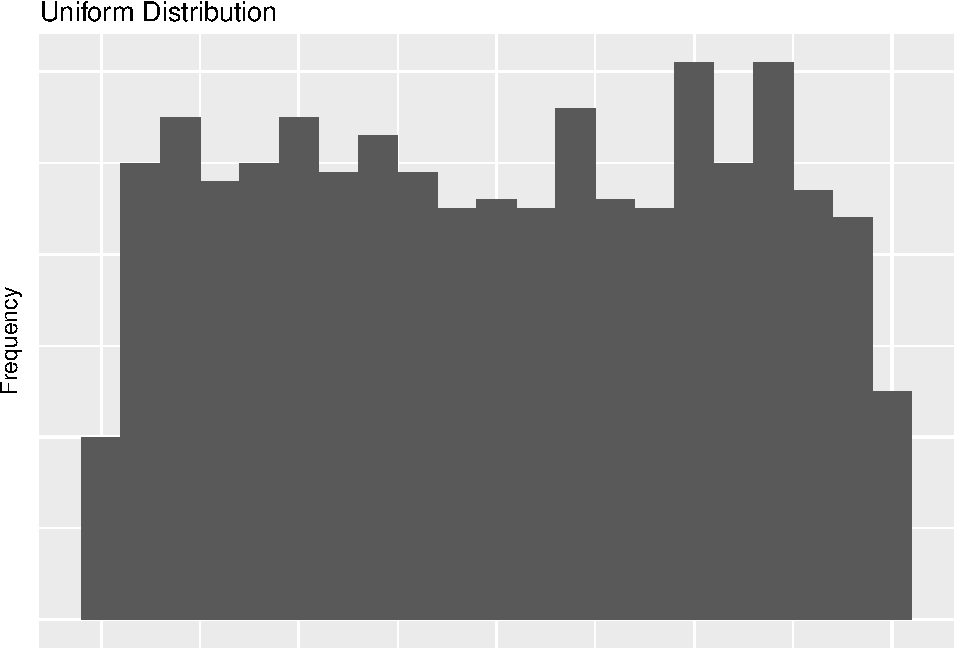
\includegraphics{bookdown-demo_files/figure-latex/unnamed-chunk-20-1.pdf}

Try to run the above code with different arguments in the
\texttt{binwidth} argument. You'll notice that the way you plot the data
will actually represent it differntly.

We can also have \textbf{positively skewed} and \textbf{negatively
skewed} distributions. If a distribution is skewed, it usually means
that the \textbf{mode} does not equal the \textbf{mean}. We're going to
approximate both of these with another one of R's probability functions.

\begin{Shaded}
\begin{Highlighting}[]
\NormalTok{positiveSkewData <-}\StringTok{ }\KeywordTok{rchisq}\NormalTok{(}\DecValTok{1000}\NormalTok{,}\DecValTok{6}\NormalTok{) }\CommentTok{# Chi Square distributions are positively skewed}
\NormalTok{negativeSkewData <-}\StringTok{ }\OperatorTok{-}\StringTok{ }\NormalTok{positiveSkewData }\CommentTok{# Flip it!}
\NormalTok{distributions <-}\StringTok{ }\KeywordTok{data.frame}\NormalTok{(uniformData, positiveSkewData, negativeSkewData)}
\KeywordTok{ggplot}\NormalTok{(distributions, }\KeywordTok{aes}\NormalTok{(distributions}\OperatorTok{$}\NormalTok{positiveSkewData)) }\OperatorTok{+}\StringTok{ }
\StringTok{  }\KeywordTok{geom_histogram}\NormalTok{(}\DataTypeTok{binwidth =} \DecValTok{1}\NormalTok{) }\OperatorTok{+}
\StringTok{  }\KeywordTok{labs}\NormalTok{(}\DataTypeTok{x =} \StringTok{"Independent Variable"}\NormalTok{, }\DataTypeTok{y =} \StringTok{"Frequency"}\NormalTok{, }\DataTypeTok{title =} \StringTok{"Positive Skew Distribution"}\NormalTok{) }\OperatorTok{+}\StringTok{    }\NormalTok{cleanUpPlots}
\end{Highlighting}
\end{Shaded}

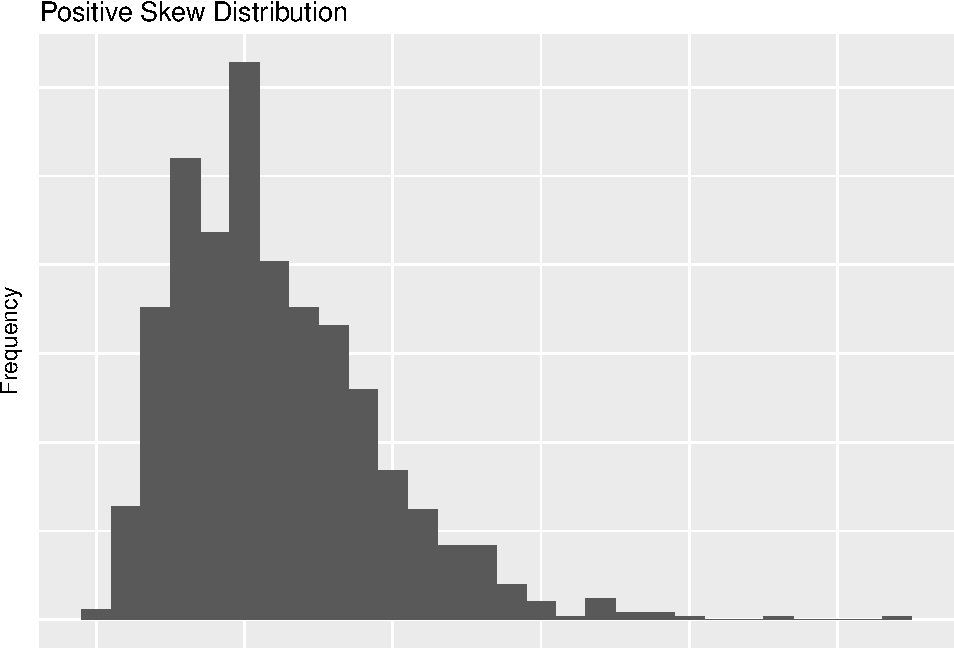
\includegraphics{bookdown-demo_files/figure-latex/unnamed-chunk-21-1.pdf}

\begin{Shaded}
\begin{Highlighting}[]
\KeywordTok{ggplot}\NormalTok{(distributions, }\KeywordTok{aes}\NormalTok{(distributions}\OperatorTok{$}\NormalTok{negativeSkewData)) }\OperatorTok{+}\StringTok{ }
\StringTok{  }\KeywordTok{geom_histogram}\NormalTok{(}\DataTypeTok{binwidth =} \DecValTok{1}\NormalTok{) }\OperatorTok{+}
\StringTok{  }\KeywordTok{labs}\NormalTok{(}\DataTypeTok{x =} \StringTok{"Independent Variable"}\NormalTok{, }\DataTypeTok{y =} \StringTok{"Frequency"}\NormalTok{, }\DataTypeTok{title =} \StringTok{"Negative Skew Distribution"}\NormalTok{) }\OperatorTok{+}\StringTok{   }\NormalTok{cleanUpPlots}
\end{Highlighting}
\end{Shaded}

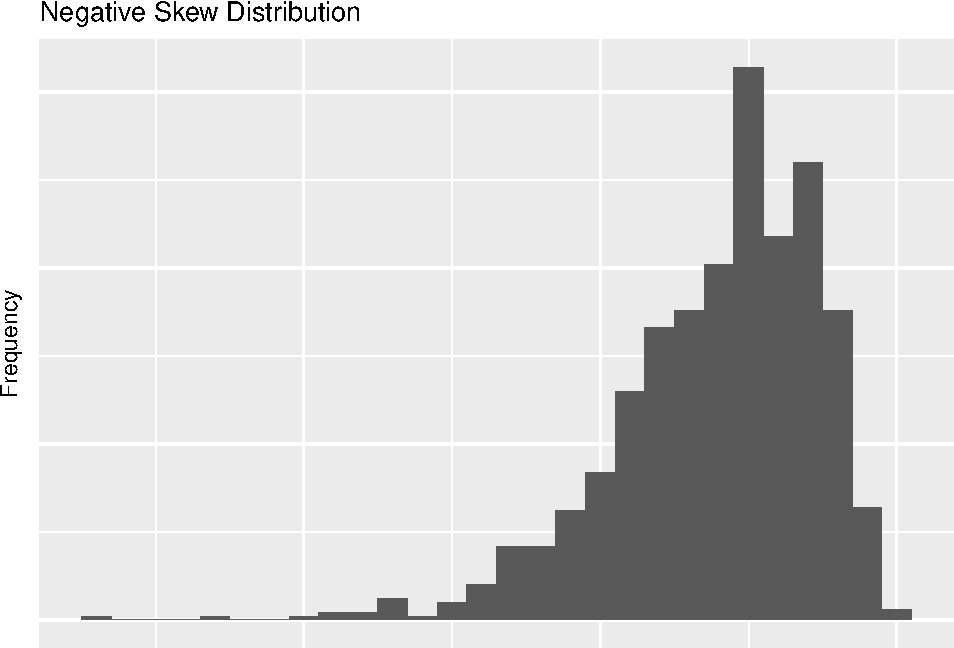
\includegraphics{bookdown-demo_files/figure-latex/unnamed-chunk-21-2.pdf}

The most important distribution in the world of Frequentist statistics
is a \textbf{normal distribution}. A normal distribution is defined by
THIS HERE.

\begin{Shaded}
\begin{Highlighting}[]
\NormalTok{normalData <-}\StringTok{ }\KeywordTok{rnorm}\NormalTok{(}\DataTypeTok{n =} \DecValTok{1000}\NormalTok{,}\DataTypeTok{mean =} \DecValTok{0}\NormalTok{,}\DataTypeTok{sd =} \DecValTok{2}\NormalTok{) }\CommentTok{# Flip it!}
\NormalTok{distributions <-}\StringTok{ }\KeywordTok{data.frame}\NormalTok{(uniformData, positiveSkewData, negativeSkewData, normalData)}
\KeywordTok{ggplot}\NormalTok{(distributions, }\KeywordTok{aes}\NormalTok{(distributions}\OperatorTok{$}\NormalTok{normalData)) }\OperatorTok{+}\StringTok{ }
\StringTok{  }\KeywordTok{geom_histogram}\NormalTok{(}\DataTypeTok{binwidth =} \DecValTok{1}\NormalTok{) }\OperatorTok{+}
\StringTok{  }\KeywordTok{labs}\NormalTok{(}\DataTypeTok{x =} \StringTok{"Independent Variable"}\NormalTok{, }\DataTypeTok{y =} \StringTok{"Frequency"}\NormalTok{, }\DataTypeTok{title =} \StringTok{"Normal Distribution"}\NormalTok{) }\OperatorTok{+}\StringTok{    }\NormalTok{cleanUpPlots}
\end{Highlighting}
\end{Shaded}

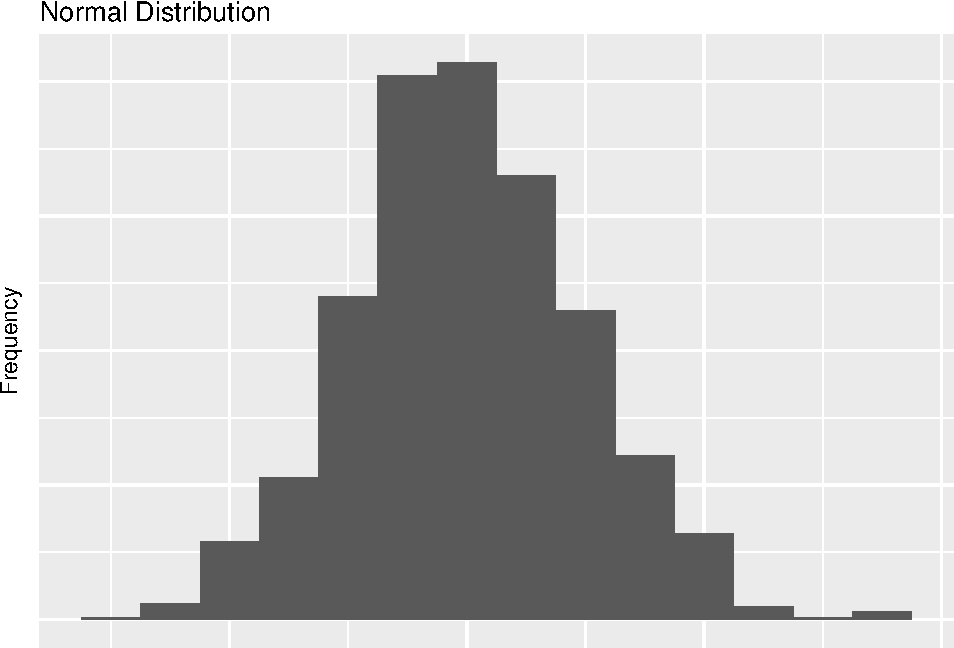
\includegraphics{bookdown-demo_files/figure-latex/unnamed-chunk-22-1.pdf}

And the lastly we can have both \textbf{leptokurtic} and
\textbf{platykurtic} distributions.

\begin{Shaded}
\begin{Highlighting}[]
\NormalTok{leptoData <-}\StringTok{ }\KeywordTok{rnorm}\NormalTok{(}\DataTypeTok{n =} \DecValTok{1000}\NormalTok{,}\DataTypeTok{mean =} \DecValTok{0}\NormalTok{,}\DataTypeTok{sd =} \DecValTok{2}\NormalTok{) }
\NormalTok{platyData <-}\StringTok{ }\KeywordTok{rnorm}\NormalTok{(}\DataTypeTok{n =} \DecValTok{1000}\NormalTok{,}\DataTypeTok{mean =} \DecValTok{0}\NormalTok{,}\DataTypeTok{sd =} \DecValTok{2}\NormalTok{)}
\NormalTok{distributions <-}\StringTok{ }\KeywordTok{data.frame}\NormalTok{(uniformData, positiveSkewData, negativeSkewData, normalData,leptoData, platyData)}
\KeywordTok{ggplot}\NormalTok{(distributions, }\KeywordTok{aes}\NormalTok{(distributions}\OperatorTok{$}\NormalTok{leptoData)) }\OperatorTok{+}\StringTok{ }
\StringTok{  }\KeywordTok{geom_histogram}\NormalTok{(}\DataTypeTok{binwidth =} \DecValTok{1}\NormalTok{) }\OperatorTok{+}
\StringTok{  }\KeywordTok{labs}\NormalTok{(}\DataTypeTok{x =} \StringTok{"Independent Variable"}\NormalTok{, }\DataTypeTok{y =} \StringTok{"Frequency"}\NormalTok{, }\DataTypeTok{title =} \StringTok{"Leptokurtic Distribution, FIX ME"}\NormalTok{) }\OperatorTok{+}\StringTok{    }\NormalTok{cleanUpPlots}
\end{Highlighting}
\end{Shaded}

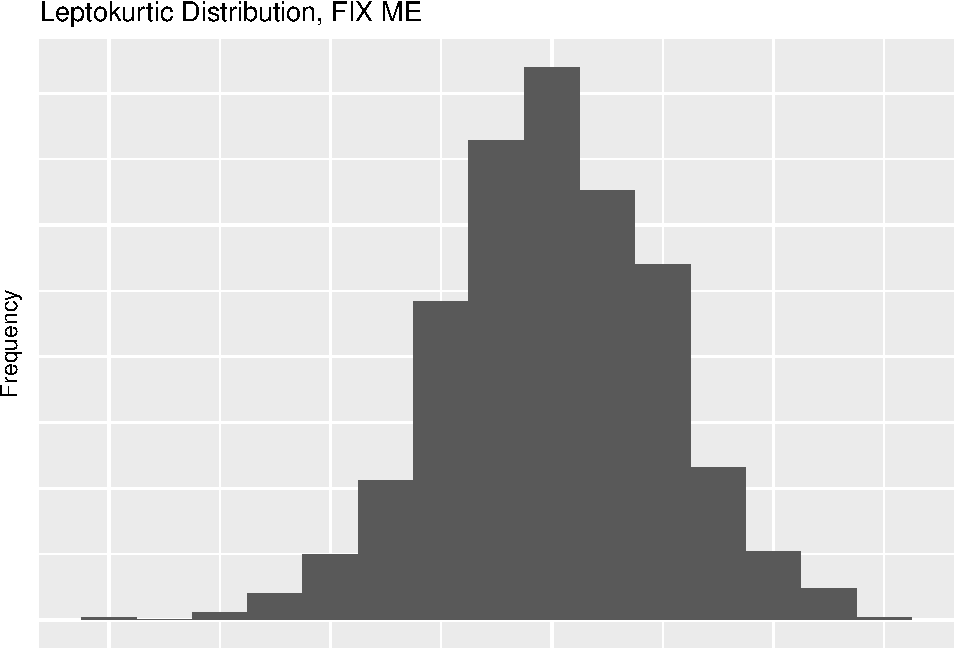
\includegraphics{bookdown-demo_files/figure-latex/unnamed-chunk-23-1.pdf}

\begin{Shaded}
\begin{Highlighting}[]
\KeywordTok{ggplot}\NormalTok{(distributions, }\KeywordTok{aes}\NormalTok{(distributions}\OperatorTok{$}\NormalTok{platyData)) }\OperatorTok{+}\StringTok{ }
\StringTok{  }\KeywordTok{geom_histogram}\NormalTok{(}\DataTypeTok{binwidth =} \DecValTok{1}\NormalTok{) }\OperatorTok{+}
\StringTok{  }\KeywordTok{labs}\NormalTok{(}\DataTypeTok{x =} \StringTok{"Independent Variable"}\NormalTok{, }\DataTypeTok{y =} \StringTok{"Frequency"}\NormalTok{, }\DataTypeTok{title =} \StringTok{"Platykurtic Distribution, FIX ME"}\NormalTok{) }\OperatorTok{+}\StringTok{    }\NormalTok{cleanUpPlots}
\end{Highlighting}
\end{Shaded}

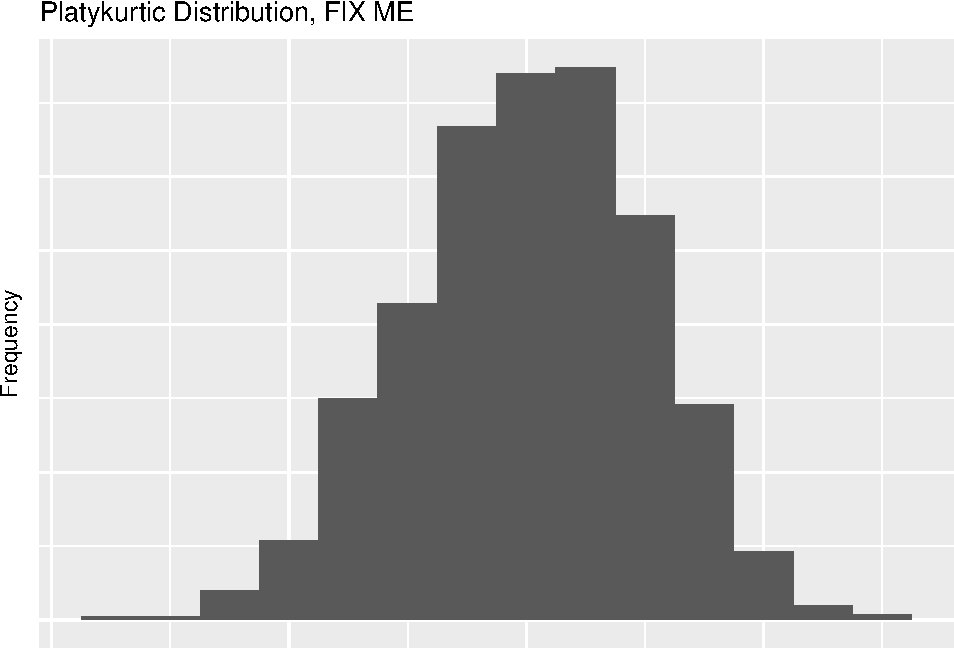
\includegraphics{bookdown-demo_files/figure-latex/unnamed-chunk-23-2.pdf}

Generally measurses of \textbf{central tendency} are used to
characterize the most typical score in a distribution.

For example we could calculate the \textbf{mean} or the \textbf{median}
of our SAT data. The mean is calculated by adding up all our numbers,
designated with the Greek letter Sigma \(\Sigma\) then dividing by the
amount of numbers we added up, or \(n\). As an equation it would look
like this.

\[\bar{X} = \frac{(\Sigma\ x_i)}{n}\]

Take a second to talk yourself through that so later you will start to
feel more comfortable with more complex equational notation. Some people
find it helpful to just try to say the equation in plain English. In
this case it would be the mean, or \(\bar{x}\) is defined as or equal to
what happens when you add up \(\Sigma\) every single value \(x\) that
you have going up to \(i\), then divide all those numbers by the amount
of numbers you have, or \(n\).

The median is defined by finding the middle number. If there is a tie
because we have an even set of numbers, we take the mean of the middle
two numbers.

We can do both of these in R as well. Below we can either type in the
numbers as you would with a calculator, or use a function in R. Notice
that each step when its typed out is saved into an object. By starting
to think this way, it will pave the way for writing more elegant code
later on.

\begin{Shaded}
\begin{Highlighting}[]
\CommentTok{# Typing it out }
\NormalTok{our.data <-}\StringTok{ }\KeywordTok{c}\NormalTok{(}\DecValTok{480} \OperatorTok{+}\StringTok{ }\DecValTok{530} \OperatorTok{+}\StringTok{ }\DecValTok{560} \OperatorTok{+}\StringTok{ }\DecValTok{650} \OperatorTok{+}\StringTok{ }\DecValTok{720} \OperatorTok{+}\StringTok{ }\DecValTok{760}\NormalTok{)}
\NormalTok{how.many <-}\StringTok{ }\KeywordTok{length}\NormalTok{(our.data)}
\NormalTok{our.data}\OperatorTok{/}\NormalTok{how.many}
\end{Highlighting}
\end{Shaded}

\begin{verbatim}
## [1] 3700
\end{verbatim}

\begin{Shaded}
\begin{Highlighting}[]
\CommentTok{# Inbuilt functions}
\KeywordTok{mean}\NormalTok{(satData}\OperatorTok{$}\NormalTok{SAT)}
\end{Highlighting}
\end{Shaded}

\begin{verbatim}
## [1] 616.6667
\end{verbatim}

\begin{Shaded}
\begin{Highlighting}[]
\KeywordTok{median}\NormalTok{(satData}\OperatorTok{$}\NormalTok{SAT)}
\end{Highlighting}
\end{Shaded}

\begin{verbatim}
## [1] 605
\end{verbatim}

Notice here that for adding up the means by hand I could have done what
programmers call hard coded the equation in. That would have looked like
this.

\begin{Shaded}
\begin{Highlighting}[]
\NormalTok{our.answer <-}\StringTok{ }\KeywordTok{c}\NormalTok{(}\DecValTok{480} \OperatorTok{+}\StringTok{ }\DecValTok{530} \OperatorTok{+}\StringTok{ }\DecValTok{560} \OperatorTok{+}\StringTok{ }\DecValTok{650} \OperatorTok{+}\StringTok{ }\DecValTok{720} \OperatorTok{+}\StringTok{ }\DecValTok{760}\NormalTok{) }\OperatorTok{/}\StringTok{ }\DecValTok{6}
\NormalTok{our.answer}
\end{Highlighting}
\end{Shaded}

\begin{verbatim}
## [1] 616.6667
\end{verbatim}

The problem with this, is that every time you get a new SAT score you
have to both enter the score and update how many scores you are dividing
by. Whenever you see a chance to take a shortcut like this, do it! It
will save you tons of time in the future.

\subsection{Important Considerations for Central
Tendency}\label{important-considerations-for-central-tendency}

There are three big considerations to think about when choosing numbers
to represent your data.

\begin{enumerate}
\def\labelenumi{\arabic{enumi}.}
\tightlist
\item
  The mode is the most variable from sample to sample; the mean is the
  least variable
\item
  The mean is the most sensitive to extreme scores; e.g., skewed
  distributions
\item
  The mean is the most frequently used measure because \emph{The sum of
  the deviations around the mean is 0 }The sum of the squared deviations
  is the smallest around the mean, rather than the mode or median; this
  is known as the least squares principle
\end{enumerate}

\subsection{Measures of Variability}\label{measures-of-variability}

The \textbf{range} is simply the largest score minus the smallest score.
It is the crudest measure of variability. In our dataset we would
calculate it with the following code.

\begin{Shaded}
\begin{Highlighting}[]
\DecValTok{760} \OperatorTok{-}\StringTok{ }\DecValTok{480}
\end{Highlighting}
\end{Shaded}

\begin{verbatim}
## [1] 280
\end{verbatim}

\begin{Shaded}
\begin{Highlighting}[]
\CommentTok{# OR}
\KeywordTok{range}\NormalTok{(satData}\OperatorTok{$}\NormalTok{SAT)}
\end{Highlighting}
\end{Shaded}

\begin{verbatim}
## [1] 480 760
\end{verbatim}

\begin{Shaded}
\begin{Highlighting}[]
\KeywordTok{max}\NormalTok{(satData}\OperatorTok{$}\NormalTok{SAT) }\OperatorTok{-}\StringTok{ }\KeywordTok{min}\NormalTok{(satData}\OperatorTok{$}\NormalTok{SAT)}
\end{Highlighting}
\end{Shaded}

\begin{verbatim}
## [1] 280
\end{verbatim}

The interquartile rangerepresents the spread between the score at the
75th and 25th percentiles. Boxplots are often used to graphically
represent inner 50\% of the scores.

\begin{Shaded}
\begin{Highlighting}[]
\NormalTok{y <-}\StringTok{ }\NormalTok{satData}\OperatorTok{$}\NormalTok{SAT}
\NormalTok{boxplot.example <-}\StringTok{ }\KeywordTok{data.frame}\NormalTok{(}
          \DataTypeTok{x =} \DecValTok{1}\NormalTok{,}
          \DataTypeTok{y0 =} \KeywordTok{min}\NormalTok{(y),}
          \DataTypeTok{y25 =} \KeywordTok{quantile}\NormalTok{(y, }\FloatTok{0.25}\NormalTok{),}
          \DataTypeTok{y50 =} \KeywordTok{median}\NormalTok{(y),}
          \DataTypeTok{y75 =} \KeywordTok{quantile}\NormalTok{(y, }\FloatTok{0.75}\NormalTok{),}
          \DataTypeTok{y100 =} \KeywordTok{max}\NormalTok{(y)}
\NormalTok{)}

\KeywordTok{ggplot}\NormalTok{(boxplot.example, }\KeywordTok{aes}\NormalTok{(x)) }\OperatorTok{+}
\StringTok{    }\KeywordTok{labs}\NormalTok{(}\DataTypeTok{title =} \StringTok{"Example of Boxplot"}\NormalTok{) }\OperatorTok{+}\StringTok{ }\KeywordTok{geom_boxplot}\NormalTok{(}\KeywordTok{aes}\NormalTok{(}\DataTypeTok{ymin =}\NormalTok{ y0, }\DataTypeTok{lower =}\NormalTok{ y25, }\DataTypeTok{middle =}\NormalTok{ y50, }\DataTypeTok{upper =}\NormalTok{ y75, }\DataTypeTok{ymax =}\NormalTok{ y100),}
    \DataTypeTok{stat =} \StringTok{"identity"}\NormalTok{)}
\end{Highlighting}
\end{Shaded}

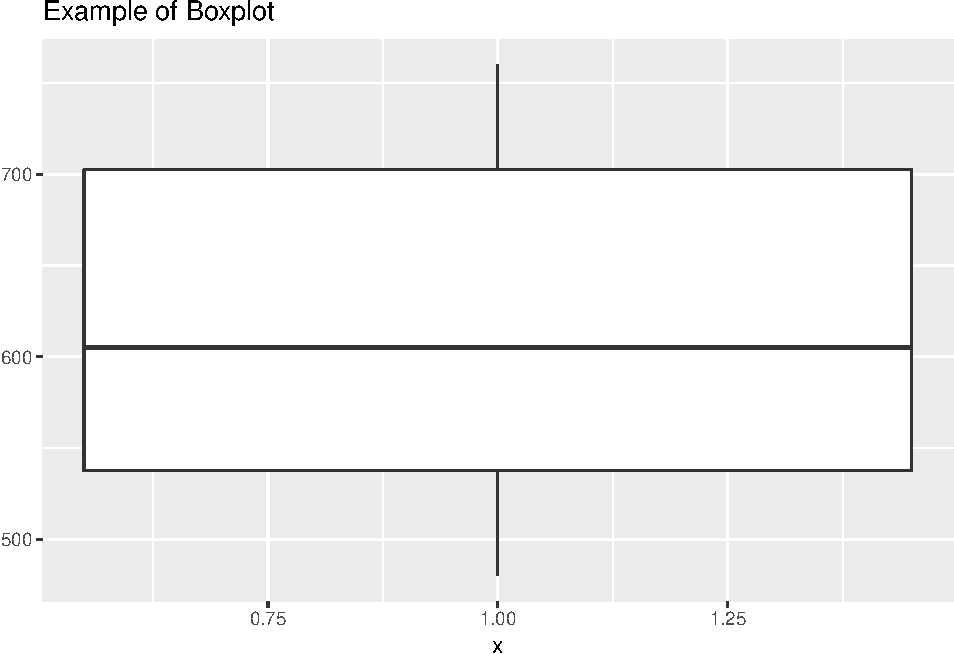
\includegraphics{bookdown-demo_files/figure-latex/unnamed-chunk-27-1.pdf}

The \textbf{variance} is essentially the averaged squared deviation
around the mean. Now there is a very important distinction that we will
get to a bit later on, but that is the difference between a
\textbf{population} value or \(\sigma^2\) and a \textbf{sample} variance
or \(s^2\). In order to do frequentist statistics, we need to assume
that there is some sort of True value that the group we are measuring
has and it is a fundamental property of the group! For more on this see
CHAPTER 3 and the work of Zoltan Dienes. Somewhere, maybe written on a
golden plate in heaven is the actual value of the average weight of a
labrador retriever. The problem is we will never have access to that
information so we need to estimate it by using a sample. The logic is
that if we can truly draw in a random way from our entire population, in
this case labrador retrievers, the central limit theroum will give us a
good approximation of what that True value will be. Since we want to be
clear about when we are talking about the Platonic, True value and the
actual sample we collected, we use different Greek notation. The
\(\sigma^2\) refers to the Platonic value and the \(\sigma^2\) is the
sample. They are defined as follows:

\[\sigma^2 = \frac{\Sigma(X_i - \mu)^2}{N}\]

\[s^2 = \frac{\Sigma(X_i - \mu)^2}{n-1}\]

Note here that each of these formulas needs a mean. In the population
equation that is defined as \(\mu\) and in samples we used \(\bar{X}\).

In our case with the SAT scores, we are wanting to know the True value
of the SAT scores of whatever population our six students are theorized
to come from. To do the calulations below we need to know the mean which
we calcualted above to be 616.67.

Now since these scores are to serve as a represntive \textbf{sample} in
hopes of getting at the true population value we need to use the formula
reflecting the \textbf{sample variance} or \(s^2\).

\[s^2 = \frac{(480-616.7)^2 + . . . + (760 - 616.676)^2}{6-1}\]

Doing this by hand we get an \(s^2\) value of 12346.67. Or running it in
R, we would use.

\begin{Shaded}
\begin{Highlighting}[]
\KeywordTok{var}\NormalTok{(satData}\OperatorTok{$}\NormalTok{SAT)}
\end{Highlighting}
\end{Shaded}

\begin{verbatim}
## [1] 12346.67
\end{verbatim}

The \textbf{standard deviation} is the square root of the variance of
the sample.

\[s = \sqrt\frac{\Sigma(X_i - \mu)^2}{n-1}\]

And since we know \(s^2\) from above, we can shorten this to

\[s = \sqrt{s^2} = \sqrt{12345.67} = 111.12\]

Or run it in R and get

\begin{Shaded}
\begin{Highlighting}[]
\KeywordTok{sd}\NormalTok{(satData}\OperatorTok{$}\NormalTok{SAT)}
\end{Highlighting}
\end{Shaded}

\begin{verbatim}
## [1] 111.1156
\end{verbatim}

\textbf{Standard scores} represent the distance of raw scores form their
mean in standard deviation units.

\[z = \frac{x_i - \bar{X}}{s}\]

So if we needed to find the \(z\) score or standardized score for
someone who got a 560 on their SAT we could compute the following.

\[z_{560} = \frac{560 - 616.67}{111.12} = -0.51\]

Interpreted in-context, this would mean that if you scored a 560 on the
SAT, based on our sample (which we think helps us get at the True
popuation value), you would be scoring about less than 1 standard
deviation (the unit of z) below the average.

\subsection{Properties of z Scores}\label{properties-of-z-scores}

Z scores are defined by having having three separte properties:

\begin{enumerate}
\def\labelenumi{\arabic{enumi}.}
\tightlist
\item
  The standardized distribution preserves the shape of the original raw
  score distribution
\item
  The mean of the standardized distribution is always 0
\item
  The variance \& standard deviation are always 1
\end{enumerate}

Many of the variables in behavioral sciences are distributed normally.
In addition, the basis for parametric inferential statistics is based on
the normal distribution.

The normal distribution is unimodal, symmetrical, bell shaped, with a
maximum height at the mean. The normal distribution is continuous and
additionallythe normal distribution is asymptotic to the X axis---it
never actually touches the X axis and theoretically goes on to infinity.

The normal distribution is really a family of distributions defined by
all possible combinations of means \(\mu\) and standard deviations
\(\sigma\). We can use the standardized normal distribution to find
areas of probability under the curve.

With a normal distribution, there is always a fixed area under the curve
which we take the reflect the probability of getting a score when
sampling from a population.

For example if we go 1 z unit (1 SD) away from the mean we find 34\% of
the total area of the curve there. If you then extend that out to the
negative side, you then encapsulate 68\% of the distribution. This would
translate to a scenario where if you were to get a score at random from
the distribution, 68\% of the time you would get a score between 1 and
-1 SD units from your mean.

This process can be extended as seen in the figure below.

\begin{figure}
\centering
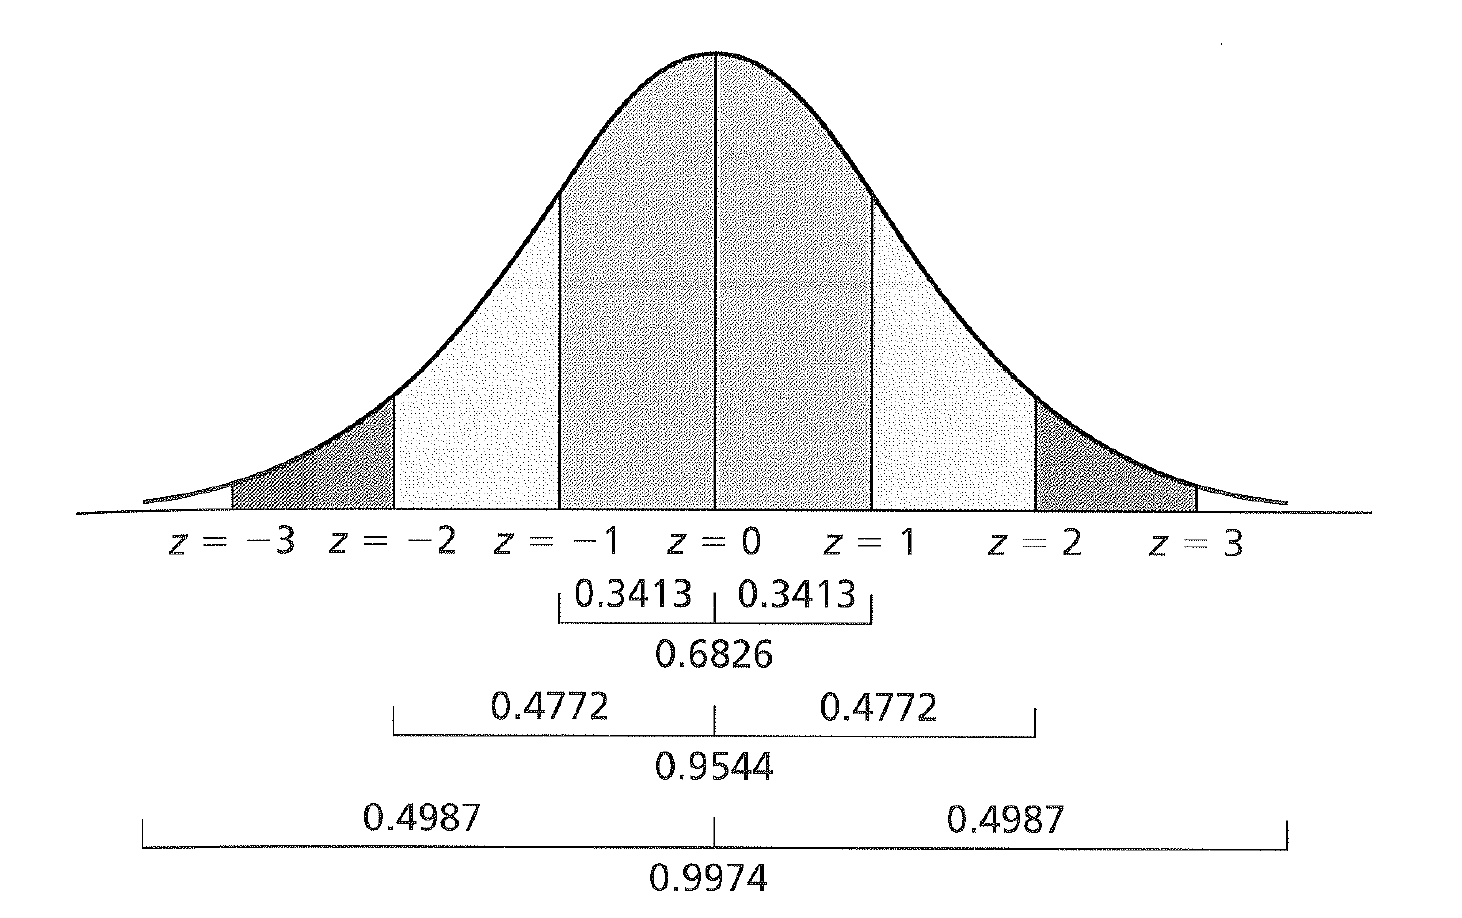
\includegraphics{img/hickszscores1.png}
\caption{z Scores and Areas Under the Curve}
\end{figure}

We could also calculate the area between two z scores as shown here.
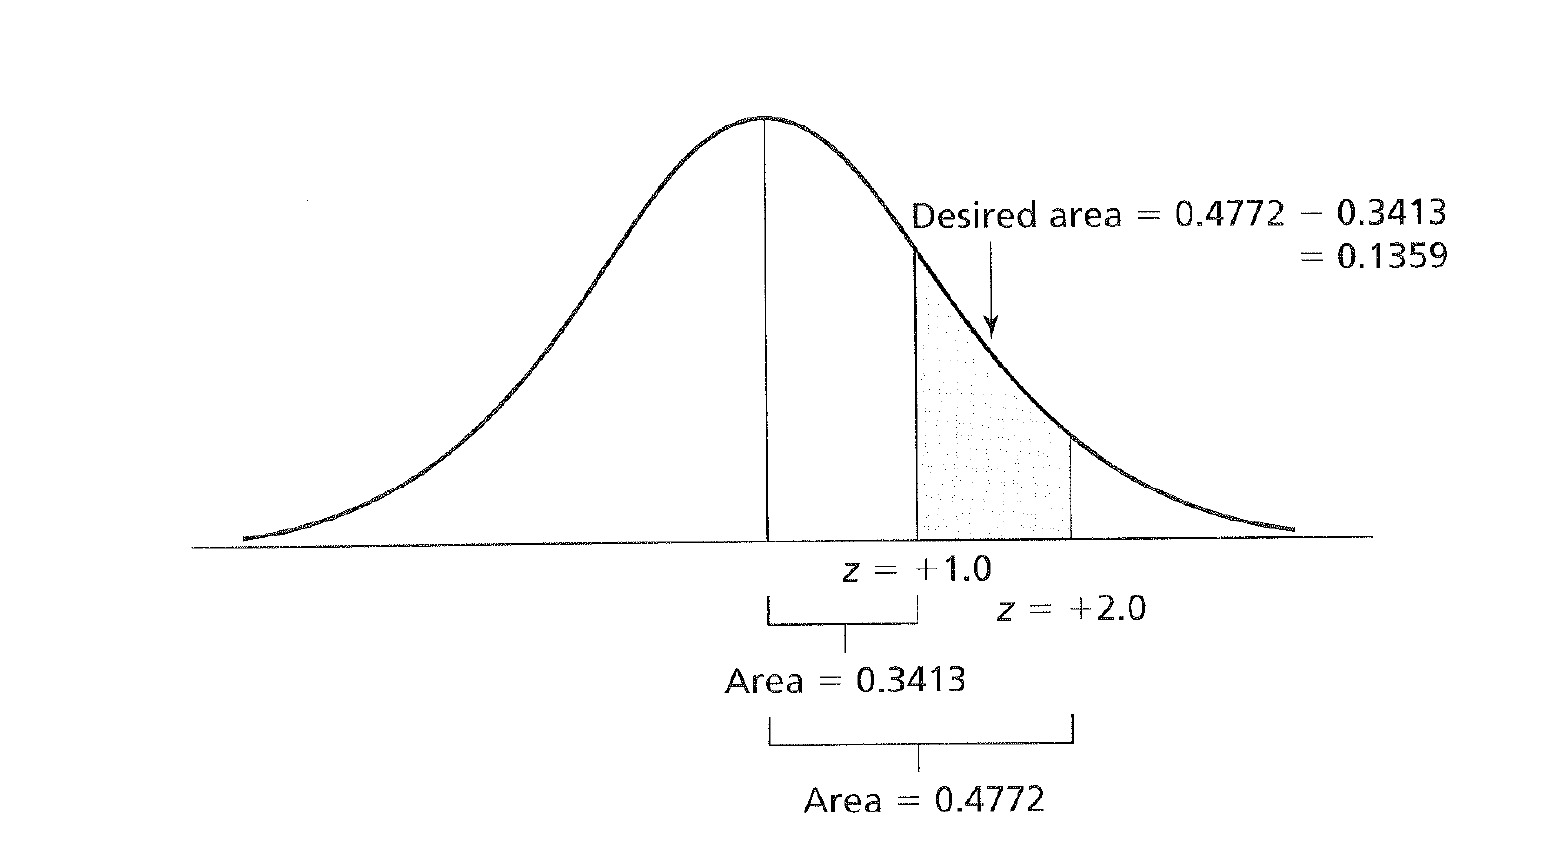
\includegraphics{img/hickszscores2.png}

And we could also look at how much area under the distribution exists
beyond two standard deviations beyond the mean.

\begin{figure}
\centering
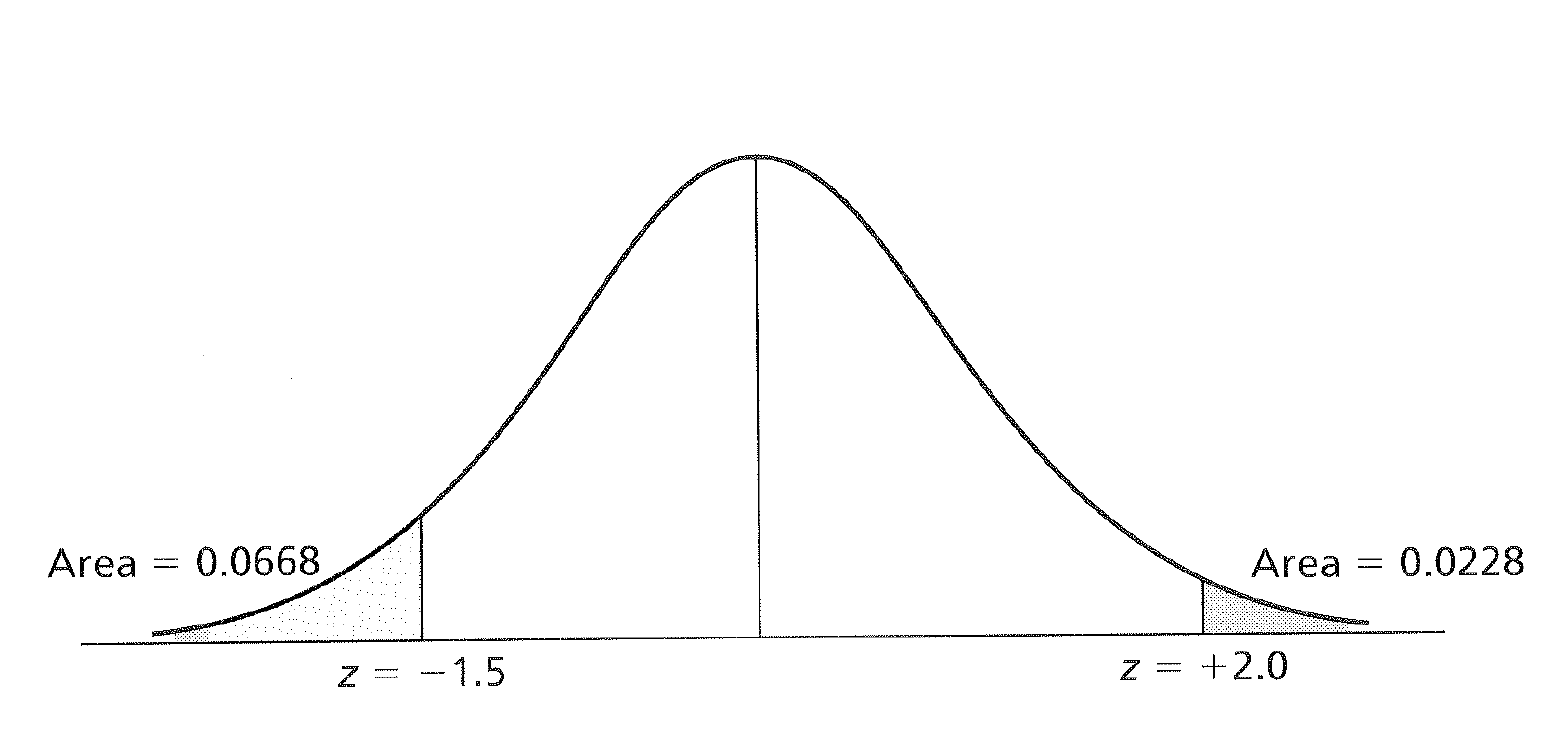
\includegraphics{img/hickszscores3.png}
\caption{z Scores and Areas Under the Curve}
\end{figure}

Or we could pick any z score values and find the area under the mean!

\begin{figure}
\centering
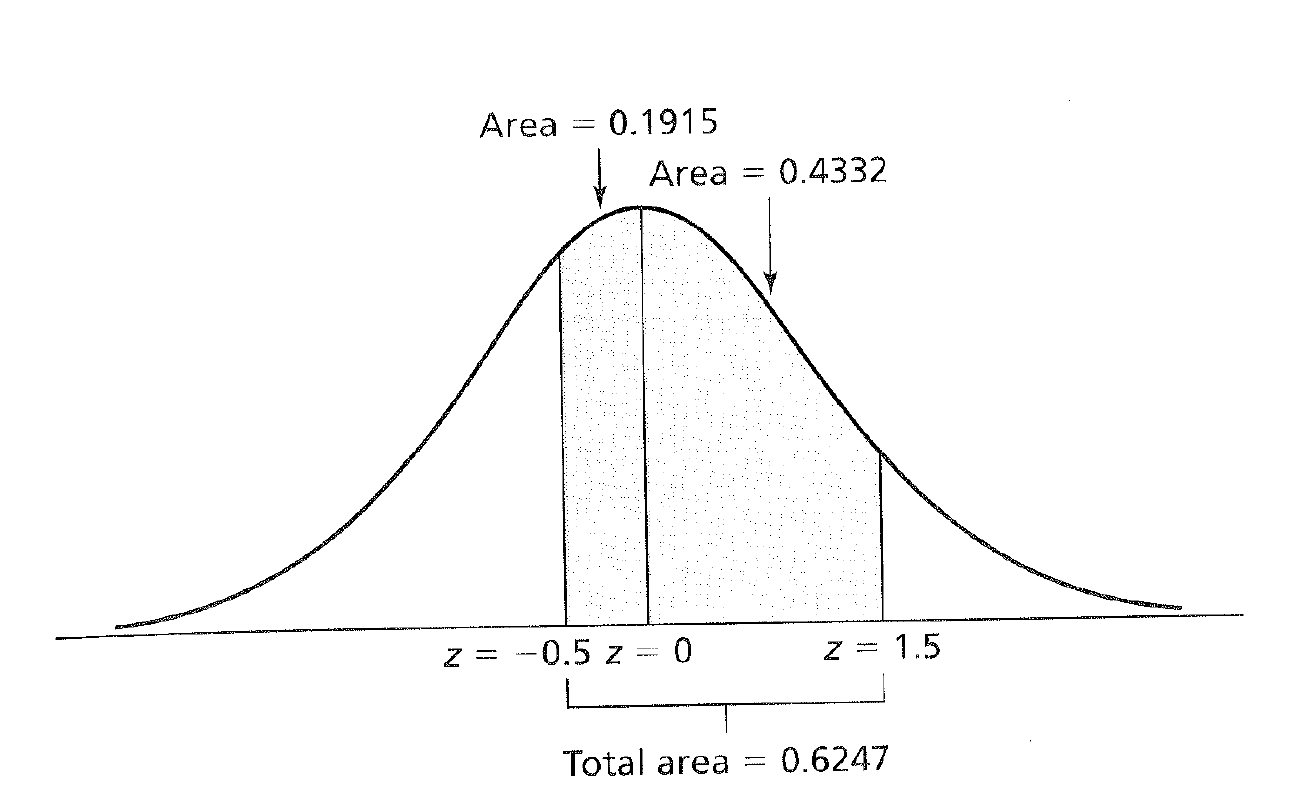
\includegraphics{img/hickszscores4.png}
\caption{z Scores and Areas Under the Curve}
\end{figure}

\section{Practice}\label{practice}

We can now start to put this to use. Here are some past homework
examples.

During tryouts, a sample of ballet dancers were rated on their athletic
ability andoverall knowledge of the art. Below are the ratings for each
dancer (a score above 75 percent means that the dancer will join the
troupe

83, 98, 45, 69, 52, 94, 82, 74, 71, 83, 62, 85, 90, 97, 61, 74, 74, 88

Let's put them into R so we can use answer a few questions about our
data.

\begin{Shaded}
\begin{Highlighting}[]
\NormalTok{ballet <-}\StringTok{ }\KeywordTok{c}\NormalTok{(}\DecValTok{83}\NormalTok{, }\DecValTok{98}\NormalTok{, }\DecValTok{45}\NormalTok{, }\DecValTok{69}\NormalTok{, }\DecValTok{52}\NormalTok{, }\DecValTok{94}\NormalTok{, }\DecValTok{82}\NormalTok{, }\DecValTok{74}\NormalTok{, }\DecValTok{71}\NormalTok{, }\DecValTok{83}\NormalTok{, }\DecValTok{62}\NormalTok{, }\DecValTok{85}\NormalTok{, }\DecValTok{90}\NormalTok{, }\DecValTok{97}\NormalTok{, }\DecValTok{61}\NormalTok{, }\DecValTok{74}\NormalTok{, }\DecValTok{74}\NormalTok{, }\DecValTok{88}\NormalTok{)}
\end{Highlighting}
\end{Shaded}

What is the median percentage?

\begin{Shaded}
\begin{Highlighting}[]
\KeywordTok{median}\NormalTok{(ballet)}
\end{Highlighting}
\end{Shaded}

\begin{verbatim}
## [1] 78
\end{verbatim}

What is the mean percentage?

\begin{Shaded}
\begin{Highlighting}[]
\KeywordTok{mean}\NormalTok{(ballet)}
\end{Highlighting}
\end{Shaded}

\begin{verbatim}
## [1] 76.77778
\end{verbatim}

What is the standard deviation for the sample (assume we don't know any
population characteristics)?

\begin{Shaded}
\begin{Highlighting}[]
\KeywordTok{sd}\NormalTok{(ballet)}
\end{Highlighting}
\end{Shaded}

\begin{verbatim}
## [1] 15.02373
\end{verbatim}

Demonstrate the least squares principle by showing that the sum of
squares (SS) around the mean is smaller than the sum of squares around
the median (remember to show your work for each).

\begin{Shaded}
\begin{Highlighting}[]
\NormalTok{ballet_mean <-}\StringTok{ }\KeywordTok{mean}\NormalTok{(ballet)}
\NormalTok{ballet_median <-}\StringTok{ }\KeywordTok{median}\NormalTok{(ballet)}
\NormalTok{ballet_sd <-}\StringTok{ }\KeywordTok{sd}\NormalTok{(ballet)}
\end{Highlighting}
\end{Shaded}

Now we can use these values to do our math!

\begin{Shaded}
\begin{Highlighting}[]
\KeywordTok{sum}\NormalTok{((ballet }\OperatorTok{-}\StringTok{ }\NormalTok{ballet_mean)}\OperatorTok{^}\DecValTok{2}\NormalTok{)}
\end{Highlighting}
\end{Shaded}

\begin{verbatim}
## [1] 3837.111
\end{verbatim}

\begin{Shaded}
\begin{Highlighting}[]
\KeywordTok{sum}\NormalTok{((ballet }\OperatorTok{-}\StringTok{ }\NormalTok{ballet_median)}\OperatorTok{^}\DecValTok{2}\NormalTok{)}
\end{Highlighting}
\end{Shaded}

\begin{verbatim}
## [1] 3864
\end{verbatim}

\begin{Shaded}
\begin{Highlighting}[]
\CommentTok{# Then having R do the final work for us}
\KeywordTok{sum}\NormalTok{((ballet }\OperatorTok{-}\StringTok{ }\NormalTok{ballet_mean)}\OperatorTok{^}\DecValTok{2}\NormalTok{) }\OperatorTok{>}\StringTok{ }\KeywordTok{sum}\NormalTok{((ballet }\OperatorTok{-}\StringTok{ }\NormalTok{ballet_median)}\OperatorTok{^}\DecValTok{2}\NormalTok{)}
\end{Highlighting}
\end{Shaded}

\begin{verbatim}
## [1] FALSE
\end{verbatim}

What are the standardized (z) scores for the raw scores 73, 99, and 66?
If you know the population mean and the sd, you can calulate a z score
using the formula \[z =  \frac{x_i - \bar{X}}{s}\]

Or in our case

\begin{Shaded}
\begin{Highlighting}[]
\NormalTok{(}\DecValTok{73} \OperatorTok{-}\StringTok{ }\NormalTok{ballet_mean)}\OperatorTok{/}\StringTok{ }\NormalTok{ballet_sd}
\end{Highlighting}
\end{Shaded}

\begin{verbatim}
## [1] -0.2514541
\end{verbatim}

\begin{Shaded}
\begin{Highlighting}[]
\NormalTok{(}\DecValTok{99} \OperatorTok{-}\StringTok{ }\NormalTok{ballet_mean)}\OperatorTok{/}\StringTok{ }\NormalTok{ballet_sd}
\end{Highlighting}
\end{Shaded}

\begin{verbatim}
## [1] 1.479142
\end{verbatim}

\begin{Shaded}
\begin{Highlighting}[]
\NormalTok{(}\DecValTok{66} \OperatorTok{-}\StringTok{ }\NormalTok{ballet_mean)}\OperatorTok{/}\StringTok{ }\NormalTok{ballet_sd}
\end{Highlighting}
\end{Shaded}

\begin{verbatim}
## [1] -0.7173837
\end{verbatim}

What proportion of scores exceeds a raw score of 73?

\begin{Shaded}
\begin{Highlighting}[]
\KeywordTok{pnorm}\NormalTok{(}\DataTypeTok{q =} \DecValTok{73}\NormalTok{, }\DataTypeTok{mean =}\NormalTok{ ballet_mean, }\DataTypeTok{sd =}\NormalTok{  ballet_sd)}
\end{Highlighting}
\end{Shaded}

\begin{verbatim}
## [1] 0.4007315
\end{verbatim}

To get the other side of the probability we can remember that we can
treat the line above as an object!

\begin{Shaded}
\begin{Highlighting}[]
\DecValTok{1} \OperatorTok{-}\StringTok{ }\KeywordTok{pnorm}\NormalTok{(}\DataTypeTok{q =} \DecValTok{73}\NormalTok{, }\DataTypeTok{mean =}\NormalTok{ ballet_mean, }\DataTypeTok{sd =}\NormalTok{  ballet_sd)}
\end{Highlighting}
\end{Shaded}

\begin{verbatim}
## [1] 0.5992685
\end{verbatim}

What proportion of scores lies between the raw scores of 75 and 100?
Let's be clever for this one and just put the two equations together for
this one. Or if you want, you could save them into objects.

\begin{Shaded}
\begin{Highlighting}[]
\KeywordTok{pnorm}\NormalTok{(}\DataTypeTok{q =} \DecValTok{100}\NormalTok{, }\DataTypeTok{mean =}\NormalTok{ ballet_mean, }\DataTypeTok{sd =}\NormalTok{  ballet_sd) }\OperatorTok{-}\StringTok{ }\KeywordTok{pnorm}\NormalTok{(}\DataTypeTok{q =} \DecValTok{75}\NormalTok{, }\DataTypeTok{mean =}\NormalTok{ ballet_mean, }\DataTypeTok{sd =}\NormalTok{  ballet_sd)}
\end{Highlighting}
\end{Shaded}

\begin{verbatim}
## [1] 0.4860093
\end{verbatim}

\begin{Shaded}
\begin{Highlighting}[]
\KeywordTok{pnorm}\NormalTok{(}\DataTypeTok{q =} \DecValTok{76}\NormalTok{, }\DataTypeTok{mean =}\NormalTok{ ballet_mean, }\DataTypeTok{sd =}\NormalTok{  ballet_sd)}
\end{Highlighting}
\end{Shaded}

\begin{verbatim}
## [1] 0.479356
\end{verbatim}

What raw score represents the 55thpercentile? To find out what raw score
represents a percentile we can go back and use the formula from above,
just rearranged a bit.

\[z =  \frac{x_i - \bar{X}}{s}\]

or with a bit of basic algerbra

\[x_i = (z * s) + \bar{X}\]

\begin{Shaded}
\begin{Highlighting}[]
\NormalTok{(.}\DecValTok{05} \OperatorTok{*}\StringTok{ }\NormalTok{ballet_sd) }\OperatorTok{+}\StringTok{ }\NormalTok{ballet_mean}
\end{Highlighting}
\end{Shaded}

\begin{verbatim}
## [1] 77.52896
\end{verbatim}

Between what raw scores does the middle 60\% of the distribution lie?

Lastly, we then need to find first what z scores map on 30\% on either
side of the disribution, then convert those z scores to raw scores on
our data using the z score formula.

First we find the z score associated with what is 30\% left and right of
the mean (it will be the same number, only negative). In this case, it
is +/-.84.

With that established, we then first solve for x

\[-0.84 = \frac{x - 76.78}{15.02}\]

Giving us a value of 64.1 And we do it again with the positive number.

\[0.84 = \frac{x - 76.78}{15.02}\] Resulting in 89.547.

\chapter{Sampling Distributions}\label{sampling-distributions}

In this chapter, we'll cover three ideas/questions.

\begin{enumerate}
\def\labelenumi{\arabic{enumi}.}
\tightlist
\item
  What are inferential statistics and the logic behind them
\item
  What the underlying distribution of all hypothetical sample estimates
  is known as the sampling distribution, and it constitutes the third of
  the three important distributions.
\item
  Several important implications follow from an understanding of the
  sampling distribution as a normal distribution and from the central
  limit theorem
\end{enumerate}

Spoken about a bit before in the other chapter, we have both sample
statistics like \(\bar{X}\) and population parameters \(\mu\).

The idea of how frequentist inferential statistics is as follows.
Samples must be selected \emph{randomly} in order to make appropopriate
inferences about the parent population. Sample estimates must be
compared to an underlying distributionof estimates of all other
hypothetical samples of that same sizefrom the parent population. Based
on this comparison and the associated probability of obtaining certain
outcomes, inferences can be made about population parameters.

\begin{figure}
\centering
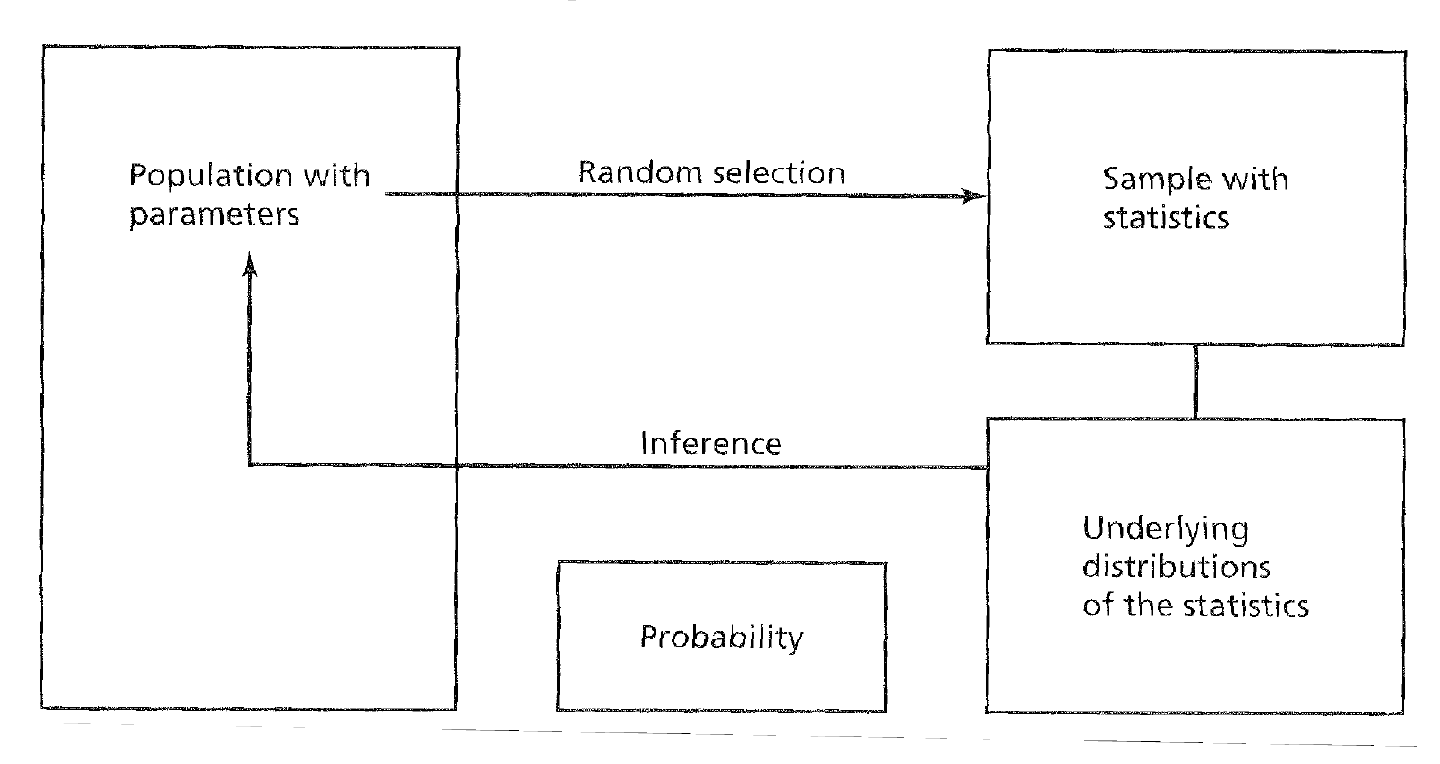
\includegraphics{img/hickssampling1.png}
\caption{Sampling}
\end{figure}

It's important to note that there are three different distributions that
we typically talk about. Two you should be familiar with -- the
populatation and the sample. The third is the \textbf{sampling
distribution} which is a \textbf{distribution of sample means}. The
sampling distribution of the mean is generated by considering all
possible sample means of a given sample size.

As is demonstratd from the image below, in A we can see there is some
sort of distribution, then with one sample (notice the \(\bar{X}\)), we
now have one wide sample. As we increase that to \(N = 16\), the
sampling distribution becomes more narrow. This narrowing is reflective
of the idea we are coming in on the true value of the population via our
random sampling. 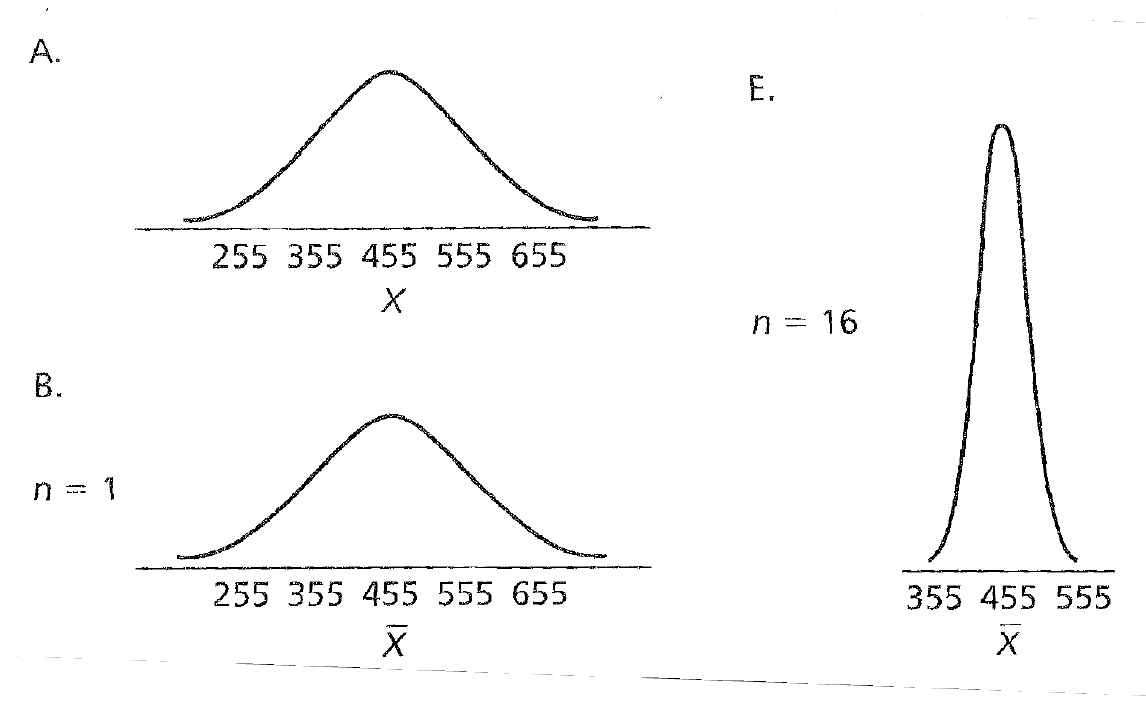
\includegraphics{img/hickssampling2.png}

The central limit theorem states that as the sample size \(n\)
increases, the sampling distribution of the mean for simple random
samples of \(n\) cases, taken from a population with a mean equal to
\(\mu\) and a finite variance equal to \(\sigma^2\), approximates a
normal distribution. From this, three points follow:

1.The shape of the sampling distribution is normal 2. The mean of the
sampling distribution is \(\mu\) 3. The standard deviation of the
sampling distribution, or standard error of the mean, is
\[\frac{\sigma}{\sqrt{n}}= \sigma_\bar{X}\]

Several important implications follow from an understanding of the
sampling distribution as a normal distribution and from the central
limit theorem.

Because we know the mean and standard error, we can calculate the
probability of selecting a random sample mean that is at or more extreme
than a particular value on the distribution.

\[z = \frac{\bar{X}-\mu}{\sigma_\bar{X}}\]

We can appeal to the table of z scores on the standard normal
distribution to find the probability.

For example, consider a sampling distribution of SAT scores with a mean
of 455 and a standard error of 8.33. This standard error was generated
with \(n\)= 144 and \(\sigma\)= 100.

So if you wanted to find the liklihood of finding as ample mean equal to
or more than extreme of 480, we would plug it into the follow equation.
\[z = \frac{480 - 455}{8.33} = 3.00\] And if we look that up a table of
z distributions, we got a probability of \(p=.0013\).

\begin{figure}
\centering
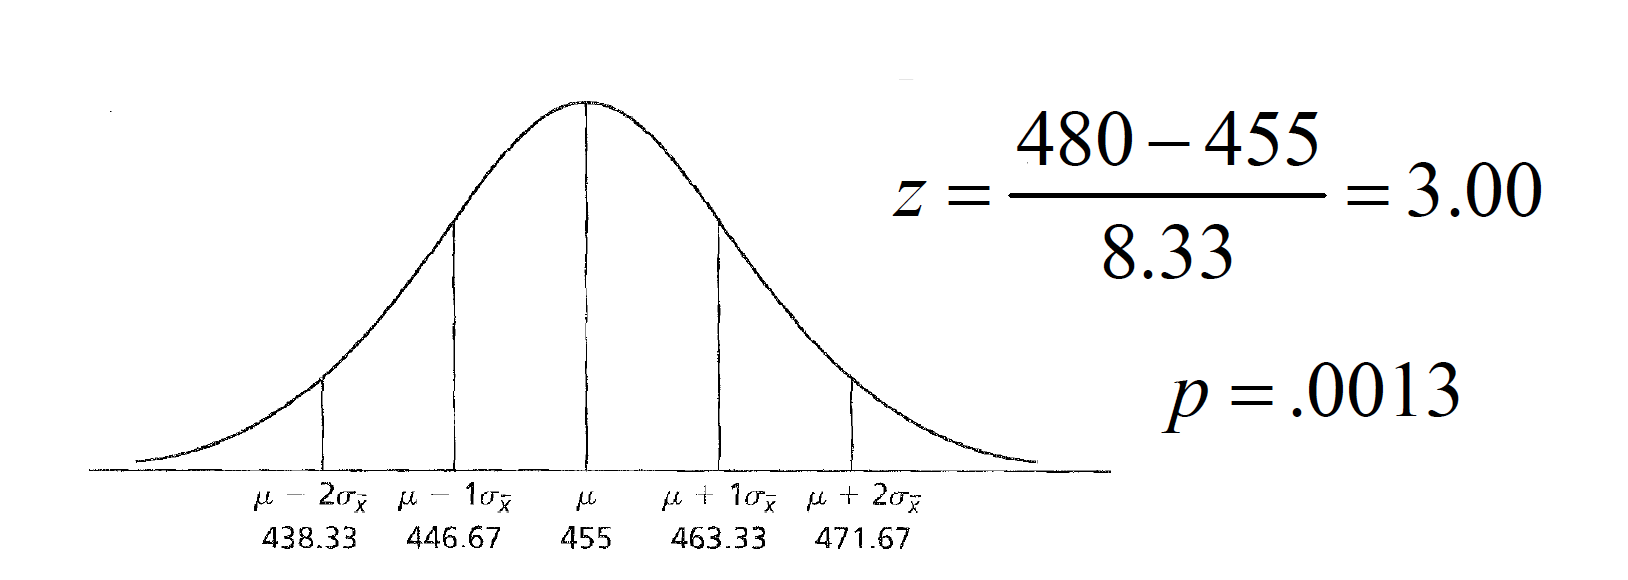
\includegraphics{img/hickssampling3.png}
\caption{Sampling}
\end{figure}

Because we know the mean and standard error, we can calculate the
probability of selecting a random sample mean that is at or more extreme
than a particular value on the distribution.

As sample size (\(n\)) increases, the variability of the sampling
distribution (\(\sigma_\bar{X}\)) decreases.

Even when the parent population is not normally distributed, the
sampling distribution becomes normal as sample size (n) increases.

You can see this demonstrated in THIS LINK.

\chapter{Hypothesis Testing}\label{hypothesis-testing}

The sampling distribution of the mean helps us to make hypotheses about
the likelihood that a given sample mean comes from a sampling
distribution with a given mean.

Stated differently, a hypothesis test helps us determine whether the
observed difference between a sample mean and a hypothetical population
mean is either negligible or meaningful.

The Null Hypothesis \(H_o : \mu = some value\) The alternative
Hypothesis \(H_o : != \mu = some value\)

The Alternative Hypothesis

A sample mean of a given sample size is produced and compared to the
hypothetical sampling distribution's mean to test the null hypothesis

Imagine we know the population (for some reason) and the True value is
455.

\begin{figure}
\centering
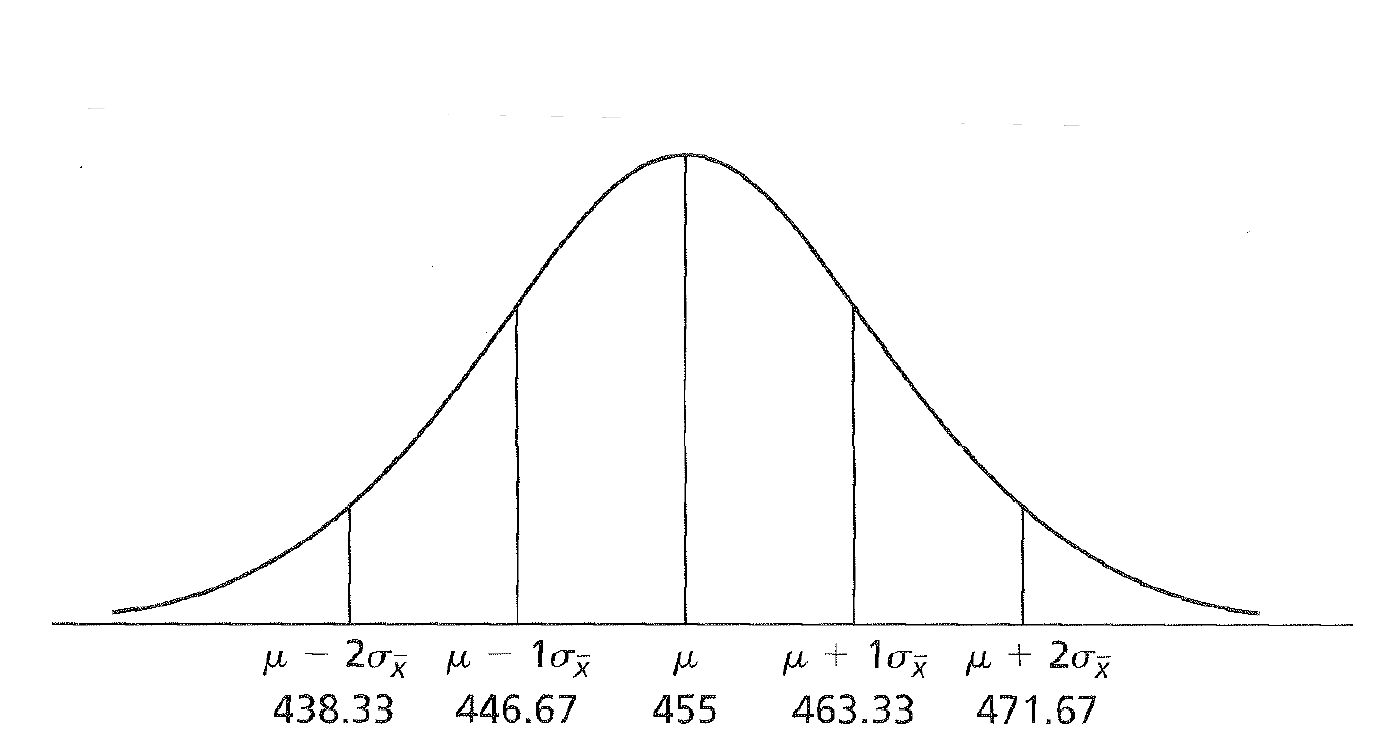
\includegraphics{img/hicksonesample1.png}
\caption{True Value is 455}
\end{figure}

\begin{figure}
\centering
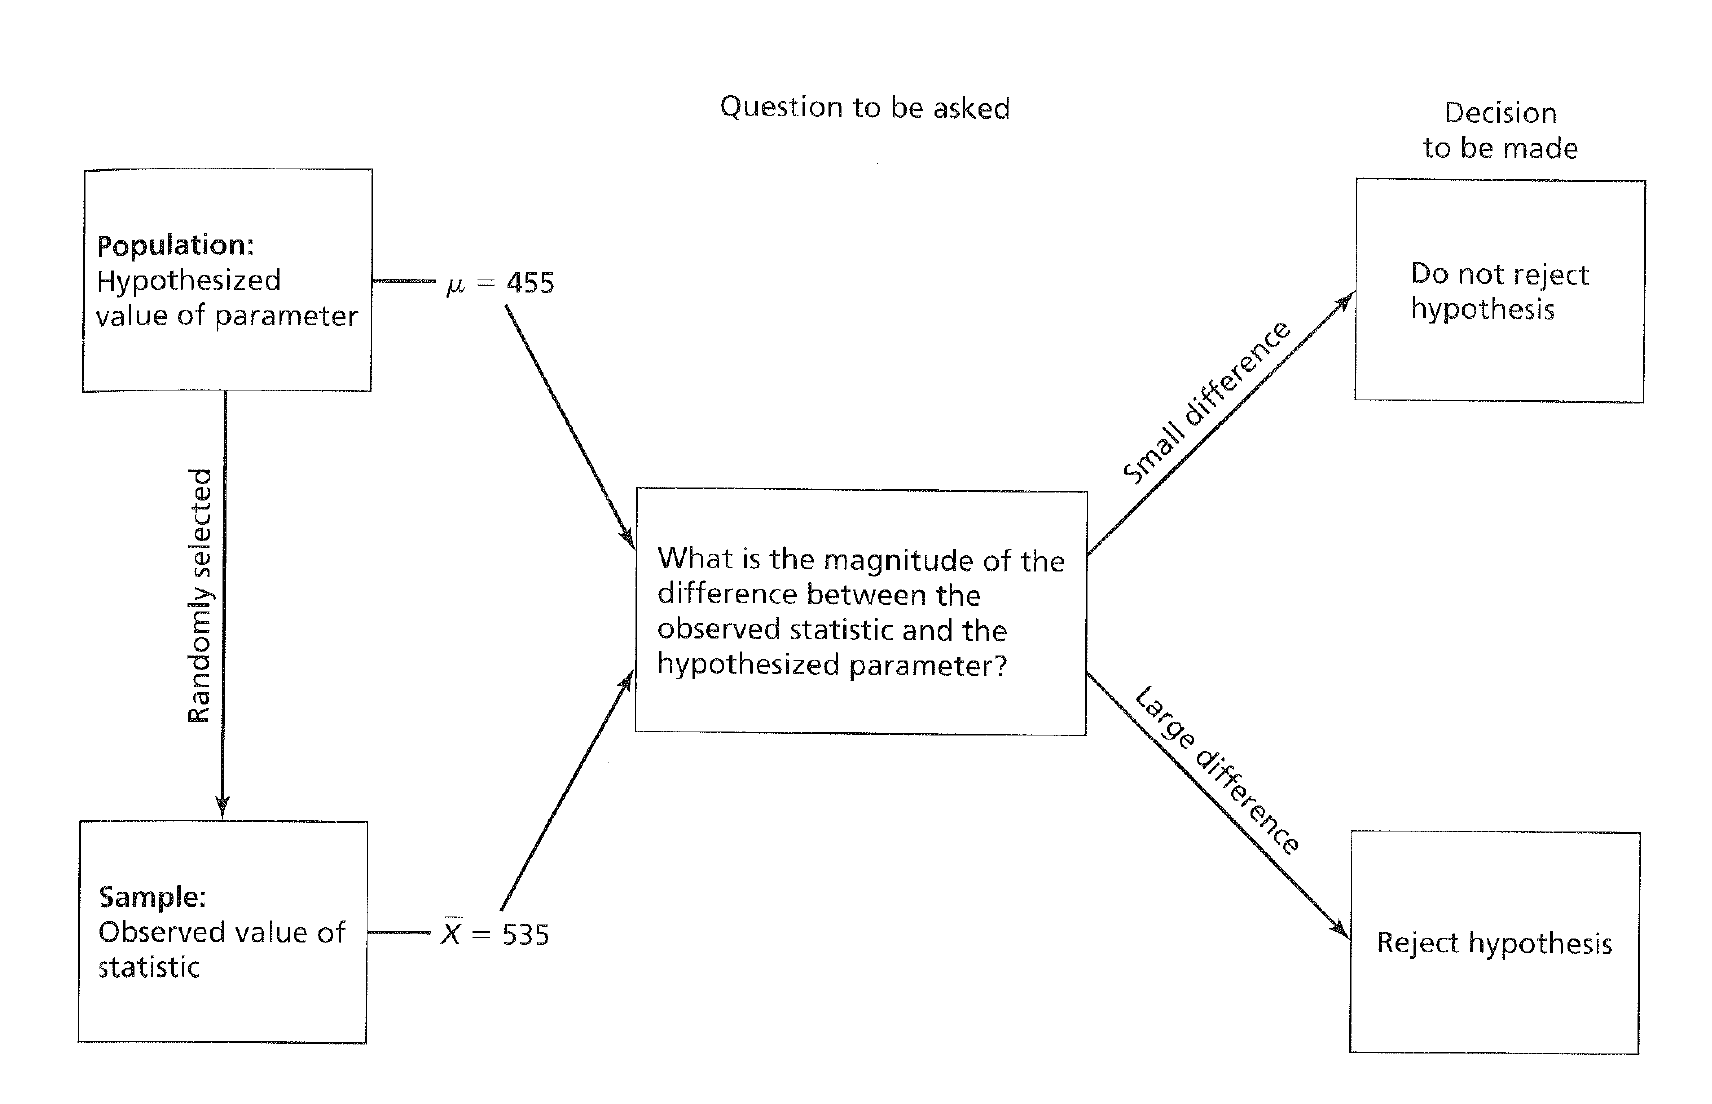
\includegraphics{img/hicksonesample2.png}
\caption{Descision Tree}
\end{figure}

The hypothesis test is based on inference (i.e., inductive reasoning),
and therefore there is a chance that mistaken inferences will be made.

The 2 ×2 matrix of decision outcomes given the state of nature and the
decision made

\begin{figure}
\centering
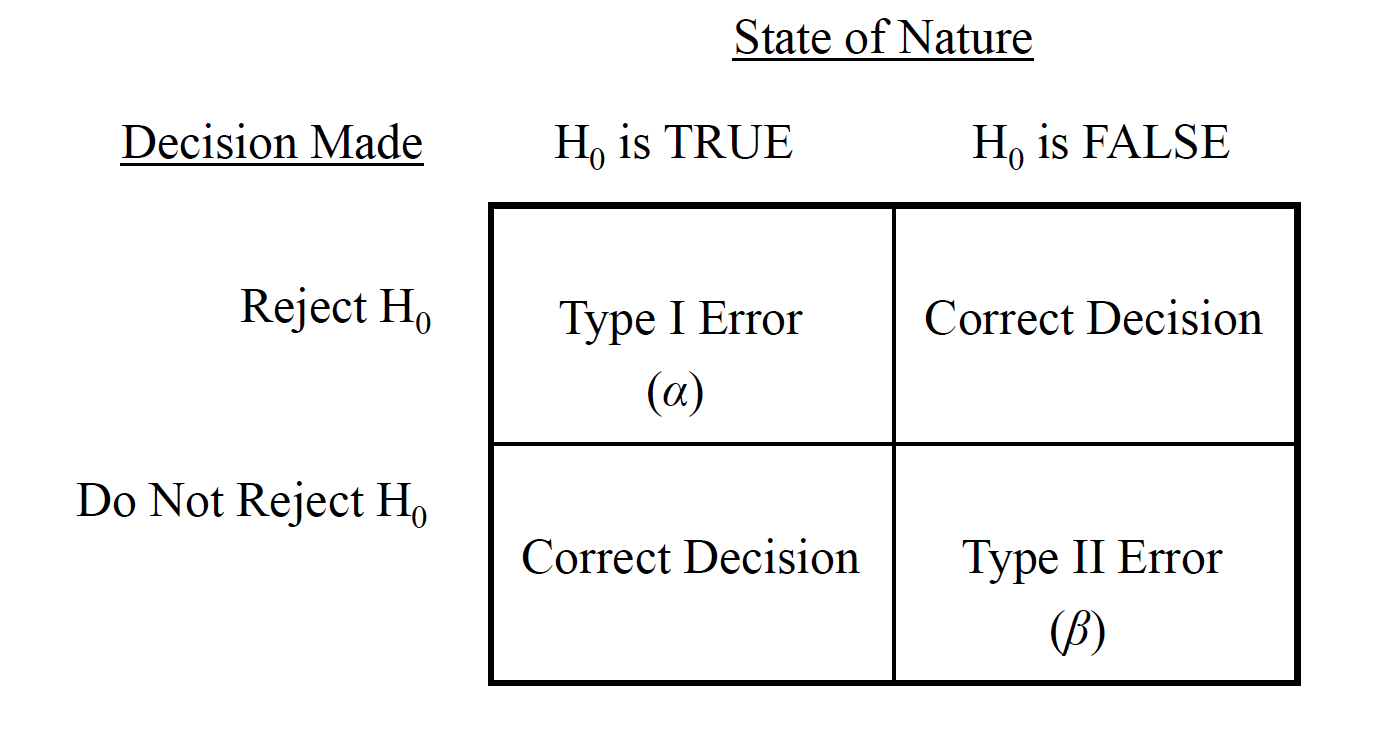
\includegraphics{img/hicksonesample3.png}
\caption{Matrix}
\end{figure}

A Type I erroris produced when we mistakenly reject the null. It is
associated with probability alpha (\(\alpha\)), or the level of
significance.

We conventionally set this level to be .05in psychology, but there are
considerations to be made for increasing or decreasing this value (e.g.,
.01 or .10).

A Type II erroris produced when we mistakenly fail to reject the null.
It is associated with probability beta (\(\beta\)), which is related to,
but not the same as, alpha.

The level of significance creates the bounds for the rejection
region---the extreme region(s) under the sampling distribution equal to
αif the null hypothesis is true.

\begin{figure}
\centering
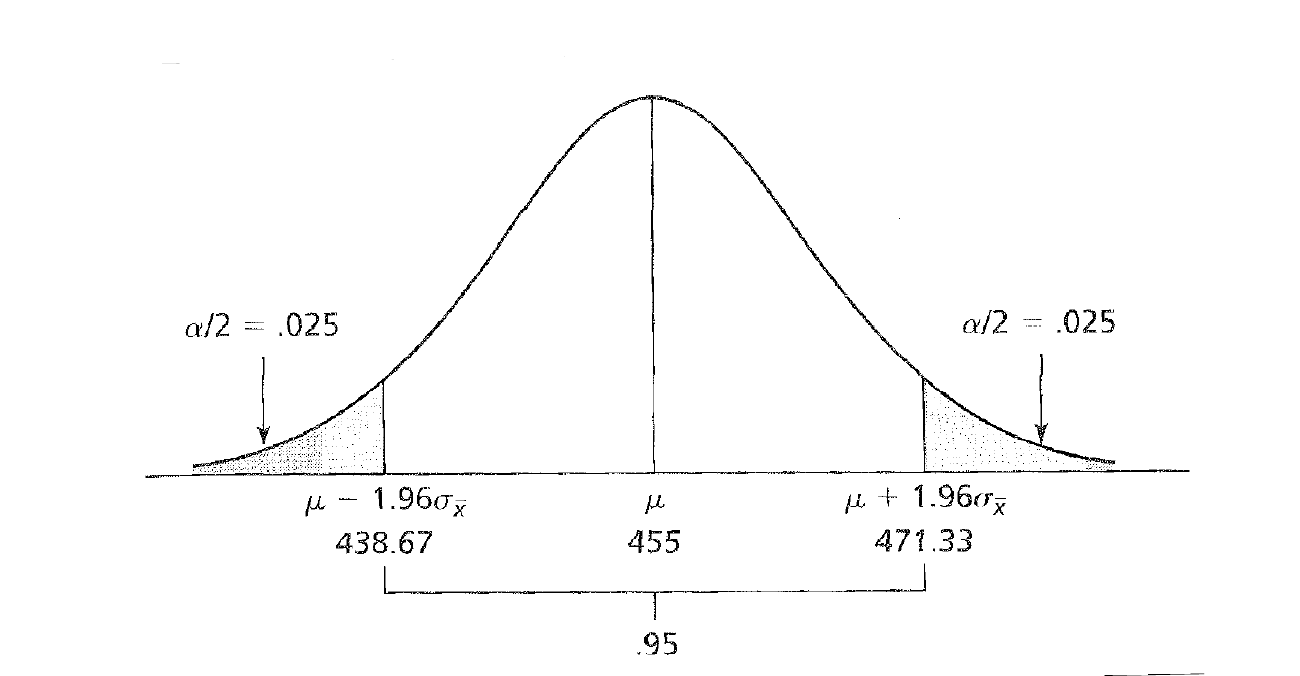
\includegraphics{img/hicksonesample4.png}
\caption{Matrix}
\end{figure}

The directionality of the test should also be considered.

\begin{figure}
\centering
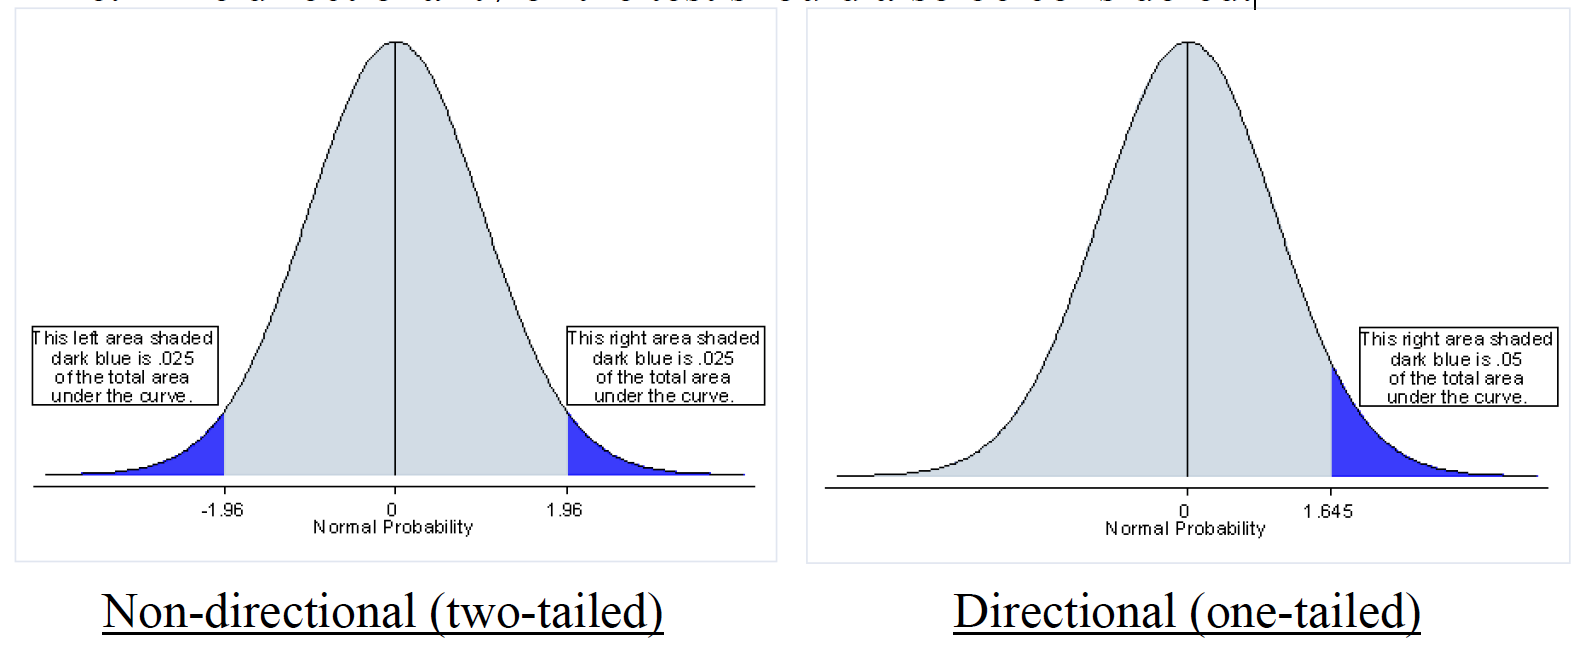
\includegraphics{img/hicksonesample5.png}
\caption{Matrix}
\end{figure}

Hypothesis tests differ slightly when population parameters, such as
\(\sigma^2\), are known versus unknown.

The general formula for a test statistic \(Statistic - parameter /SE\)

When \(\sigma^2\)is known, we use the standard error of the normal
distribution as the denominator. The result is the ztest.

Z TEST FORMULA

STANDARD ERROR HERE

When \(\sigma^2\) is unknown, we use the t distributionas our sampling
distribution, with a standard error that must be estimated from \(s^2\)
or \(s\). The result is the ttest.

T TEST AND STANDARD ERROR FORMULA HERE

Left off on Page 11 in onesampleNHST.png

The concept of degrees of freedom (df)must be considered for the ttest.
For each sample drawn, df= n--1.

VARIANCE FORMULSA

\begin{figure}
\centering
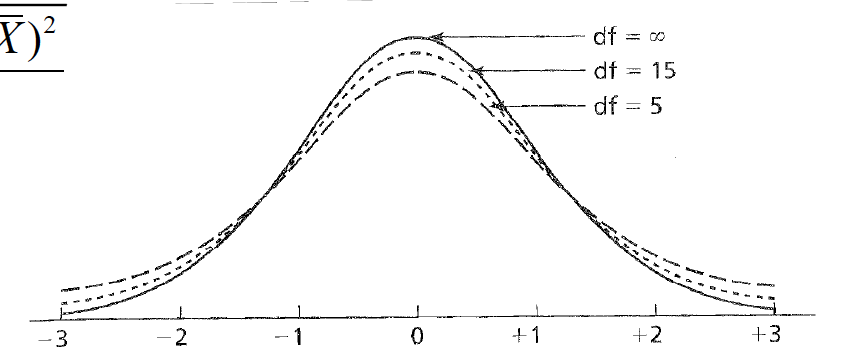
\includegraphics{img/hickssampling5.png}
\caption{DF on t statistic}
\end{figure}

\section{Steps of Hypothesis Testing}\label{steps-of-hypothesis-testing}

On a standardized anagram task, \(\mu\)= 26 anagrams solved with a
\(\simga\)= 4. A researcher tests whether the arousal from anxiety is
distracting and will decrease performance. A sample of \(n\)= 14 anxiety
patients is tested on the task. There average performance is 23.36
anagrams.

Step one: State the null and alternative hypotheses

\$H\_O = : \mu = 26 \$ \$H\_O = : \mu != 26 \$

Consider directionality.

Step two: Set the criterion for rejecting H0. Alpha is usually set to
.05, but could be other values depending on the research context. Again,
directionality is important to consider.

Step three: Select the sample and collect your data.

Step four: Locate the region of rejection and the critical value(s) of
your test statistic. Again, directionality is important to consider.

Step five: Compute the appropriate test statistic. σis known, so we use
the ztest.

\begin{figure}
\centering
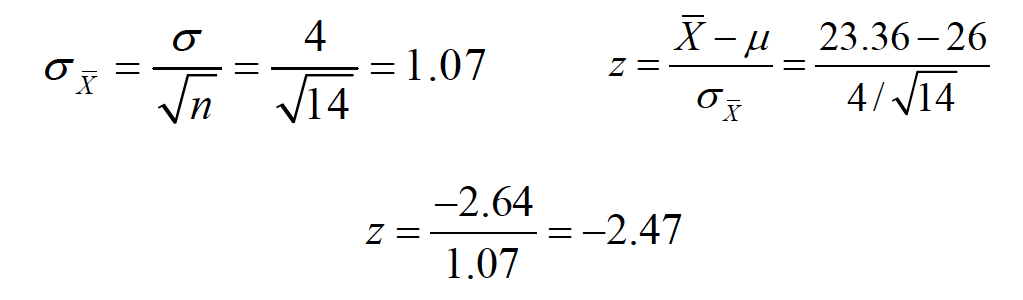
\includegraphics{img/hickssampling6.png}
\caption{Convert me}
\end{figure}

\begin{figure}
\centering
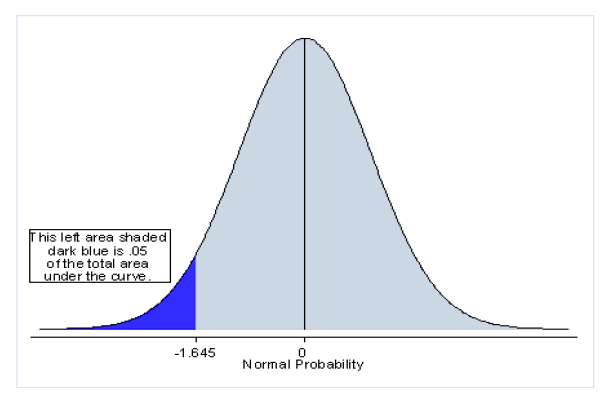
\includegraphics{img/hickssampling7.png}
\caption{Convert me}
\end{figure}

Step six: Decide whether to reject H0. Is -2.47 more extreme than the
critical value?

Step five: Compute the appropriate test statistic. \(\sigma\) is
unknown, so we use the ttest.

Step six: Decide whether to reject H0. Is -3.00 more extreme than the
critical value? df= 13, look up critical value in table C.3 and find
±1.77.

T distribution here

How do we report this result in a typical research article? ``The mean
number of anagrams solved by anxiety patients (M= 23.36) was
significantly lower than the mean established by test norms (M= 26),
t(13) = 3.00, p\textless{} .05.'' Sometimes you'll find people report
the pvalue lower than .01 if it passes this criterion as well. For
example, t(13) = 3.00, p\textless{} .01. Don't be confused by the
meaning of this, however.

\subsection{Other important
considerations.}\label{other-important-considerations.}

The hypothesis test is a test of the NULL hypothesis, assuming that the
null is true. Thus, the test gives you the probability of your sample
mean being that different (or more) from the population mean by chance
IFFthe null is true.

Statistical significance is not the same as practical significance.

Being able to report the result of a hypothesis test statistically
versus being able to describe the result to a lay person. Relate the
inference back to the original research question!

\section{Two Sample}\label{two-sample}

In cases where we wish to compare two sample means, the hypothesis
testing logic is essentially the same as with the one-sample tests, with
some slight differences in the null hypothesis, in the sampling
distribution, and in the computation. When different people (or animals)
contributed to the two samples, the comparison distribution that
represents the null hypothesis is a sampling distribution of differences
between means. The hypothesis test is therefore referred to as an
independent-samples test.

When both sample means were produced by the same participants, we
conduct what is known as a dependent-samples test. This is a test of the
average difference between the scores in one condition and the scores in
another condition---thus, the unit of measurement is a difference score.

Nondirectional Null Hypothesis \$H\_O : \mu\_1 - \mu\_2 = 0 \textbar{}
H\_O : \mu\_1 = \mu\_2 \$ Nondirectional Alternative Hypothesis \$H\_a :
\mu\_1 - \mu\_2 != 0 \textbar{} H\_a : \mu\_1 = \mu\_2 \$

Directional Null Hypothesis \$H\_O : \mu\_1 \textgreater{} \mu\_2
\textbar{} \mu\_1 \textless{} \mu\_2 \$ Directional Alternative
Hypothesis \$H\_a : \mu\_1 \textless{} \mu\_2 \textbar{} H\_a : \mu\_1
\textgreater{} \mu\_2 \$

\begin{figure}
\centering
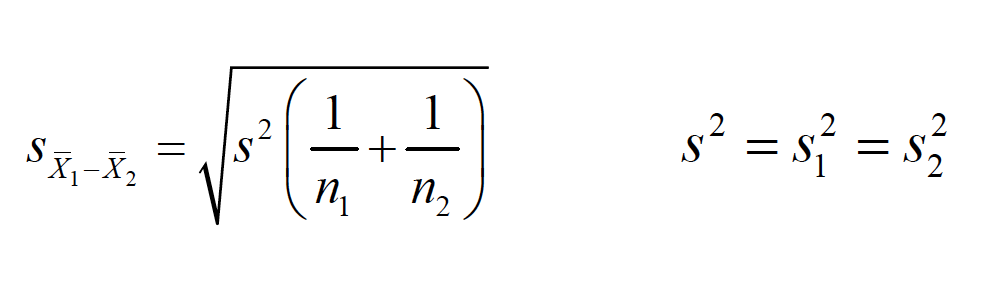
\includegraphics{img/hickssampling11.png}
\caption{Convert me}
\end{figure}

This is basically a subtraction of one sampling distribution from
another, to produce a distribution of possible differences between
sampling distributions. \$ \mu\_1 - \mu\_2\$ * The mean of this sampling
distribution is \$ \mu\_1 - \mu\_2\$ * The shape of this sampling
distribution is approximately normal. * When \sigma 2is known for each
distribution, the standard error of the difference between means is

s2is considered a pooled estimateof the population variance because the
individual estimates are literally summed together in the computation:

\(s^2 = \frac{SS_1 + SS_2}{n_1 + n_2 -2}\)

If you know the individual group variances or standard deviations, then

\(s^2 = \frac{(n_1 - 1)s_1^2 + (n_2 - 1)s_2^2}{n_1 + n_2 -2}\)

\begin{figure}
\centering
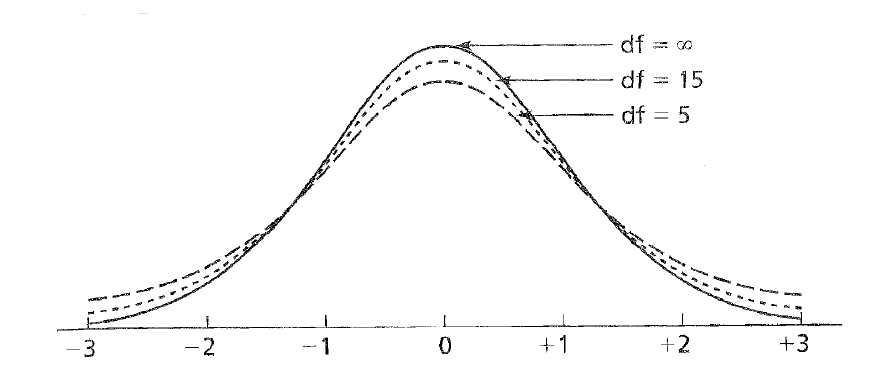
\includegraphics{img/hickssampling12.png}
\caption{Convert me}
\end{figure}

\(t = \frac{(\bar{X_1}-\bar{X_2})-(\bar{\mu_1}-\bar{\mu_2})}{s_{\bar{X_1}-\bar{X_2}}}\)

Example of the independent samples ttest

The instructor of an introductory psychology course is interested in
knowing if there is a difference in the mean grades on the final exam
between the fall and spring semester classes. Summary data for the two
samples is below:

\begin{figure}
\centering
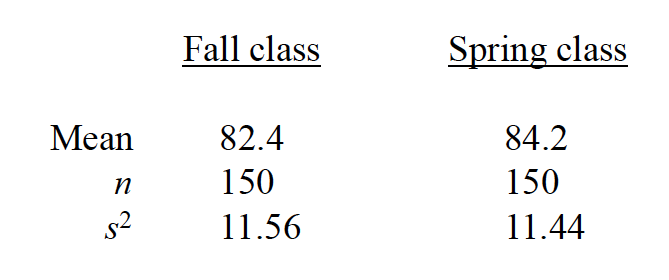
\includegraphics{img/hickssampling13.png}
\caption{Convert me}
\end{figure}

Are the final exam grades for the two classes equivalent?

Step one: State the null and alternative hypotheses
\(H_o:\mu_1 = \mu_2\) \(H_a:\mu_1 != \mu_2\)

b.Step two: Set the criterion for rejecting H0. Alpha is usually set to
.05, but could be other values depending on the research context. Make
sure you've considered directionality! c.Step three: Select the sample
and collect your data. d.Step four: Locate your region of rejection and
critical values.

Locate your region of rejection and critical values.

\(t_{cv,dv=298, \alpha=.05}= +/- 1.96\)

Step five: Compute the appropriate statistic. We were never given
\(\sigma\) or \(\sigma^2\), so we use the t test.

\begin{figure}
\centering
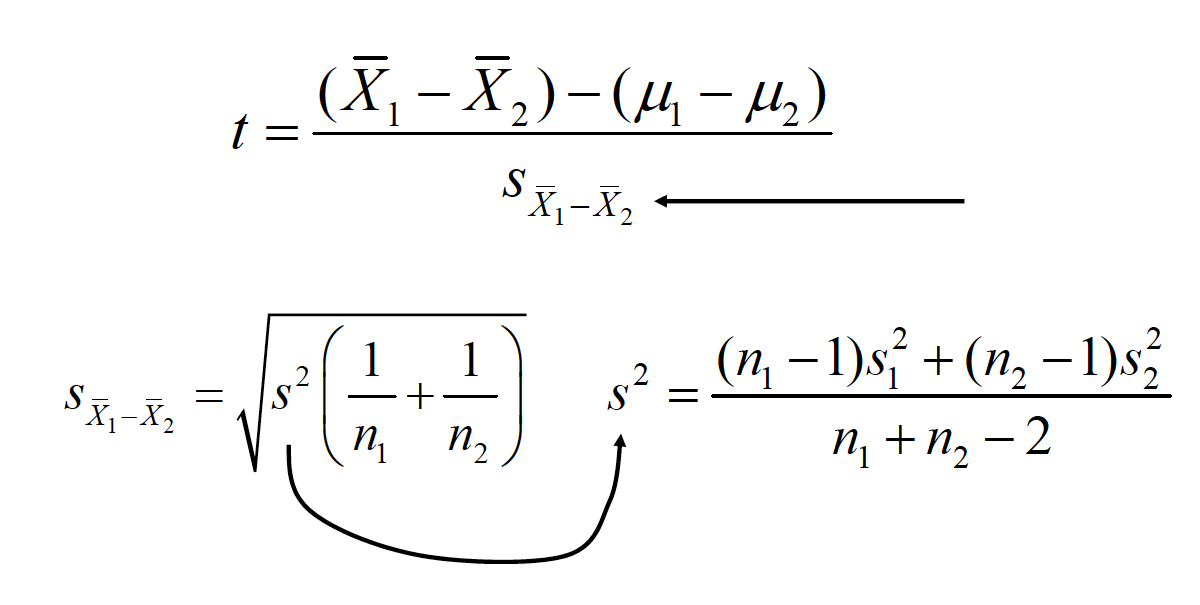
\includegraphics{img/hickssampling14.png}
\caption{Convert me}
\end{figure}

\begin{figure}
\centering
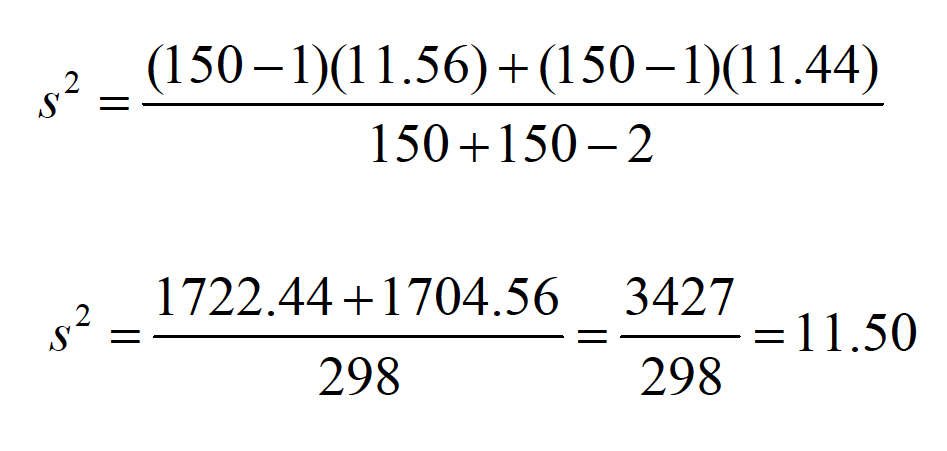
\includegraphics{img/hickssampling15.png}
\caption{Convert me}
\end{figure}

\begin{figure}
\centering
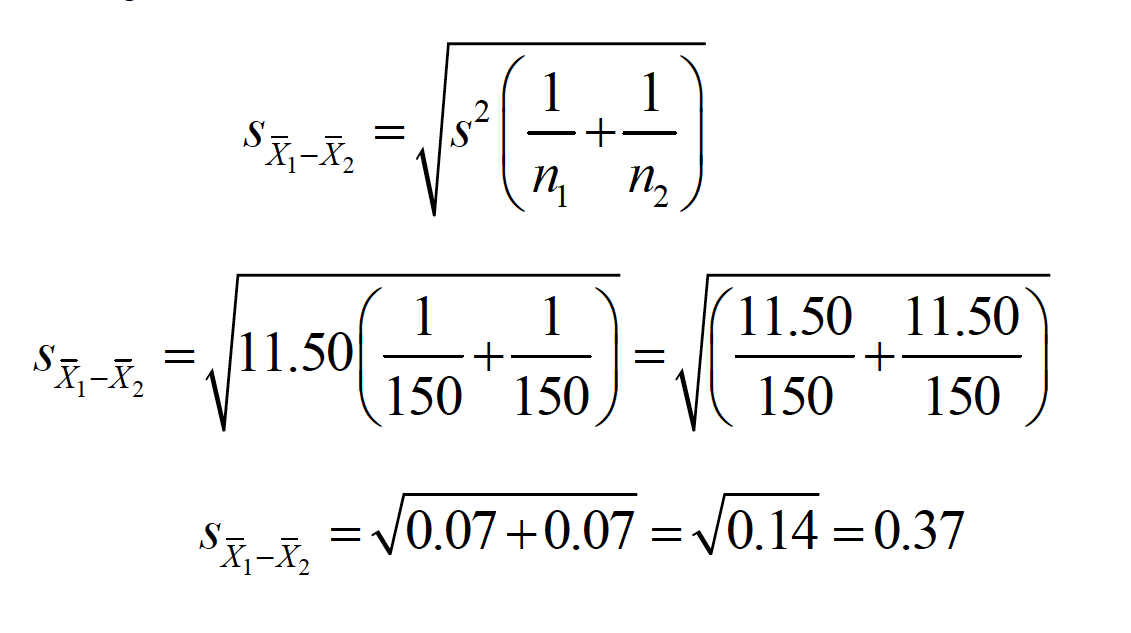
\includegraphics{img/hickssampling16.png}
\caption{Convert me}
\end{figure}

\begin{figure}
\centering
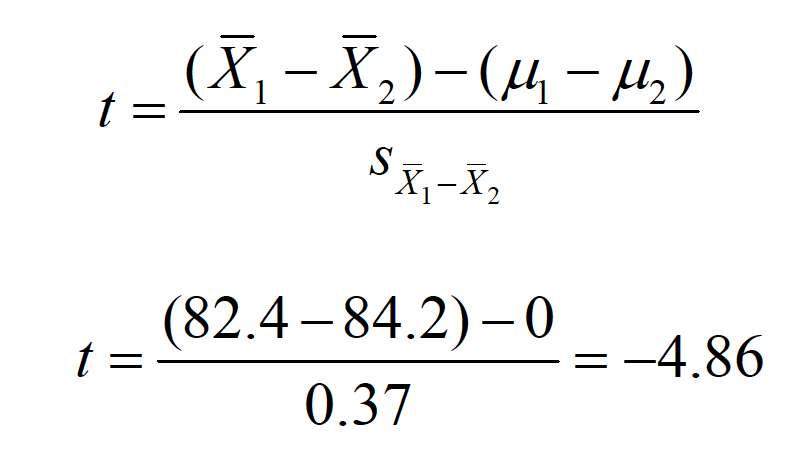
\includegraphics{img/hickssampling17.png}
\caption{Convert me}
\end{figure}

Step six: Decide whether to reject H0. Is -4.86 more extreme than the
critical value?

\(t_{cv,dv=298, \alpha=.05}= +/- 1.96\)

The effect sizerefers to the magnitude of the phenomenon being tested
and is calculated as

\begin{figure}
\centering
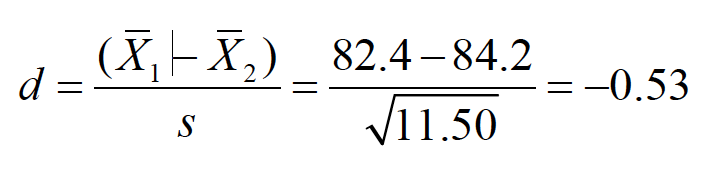
\includegraphics{img/hickssampling18.png}
\caption{Convert me}
\end{figure}

This statistic reflects the standardized distance between two
populationmeans. J. Cohen provides guidelines to interpret the value of
d:

``The average final exam score from the fall semester (M= 82.4) was
significantly lower than the average score from the spring semester (M=
84.2), t(298) = 4.86, p\textless{} .05.''

Small: = 0.25Medium: = 0.50Large: = 1.0

``The average final exam score from the fall semester (M= 82.4) was
significantly lower than the average score from the spring semester (M=
84.2), t(298) = 4.86, p\textless{} .05, Cohen's d= 0.53.''

\chapter{Power, Confidence Intervals, Effect Size
Measures}\label{power-confidence-intervals-effect-size-measures}

\section{Power}\label{power}

We have discussed the fact that the conclusions drawn from hypothesis
tests are essentially inferences about population parameters, based on
sample information. But we have thus far neglected a discussion of what
statistical factors should be considered in planning and assessing
research-based hypothesis tests.

By minimizing the probability of a Type II error (β), we are at the same
time increasing the amount of powerof our hypothesis test (1-β). Power
is defined as the probability of rejecting the null hypothesis when it
is false (i.e., should be rejected). Four important factors affect the
power of a statistical test.

Knowing any three of these factors mathematically fixes the fourth.
Thus, one can use these factors in determining the appropriate design
for a particular study. Sample size is most often the targeted factor in
formulating such a plan.

\begin{figure}
\centering
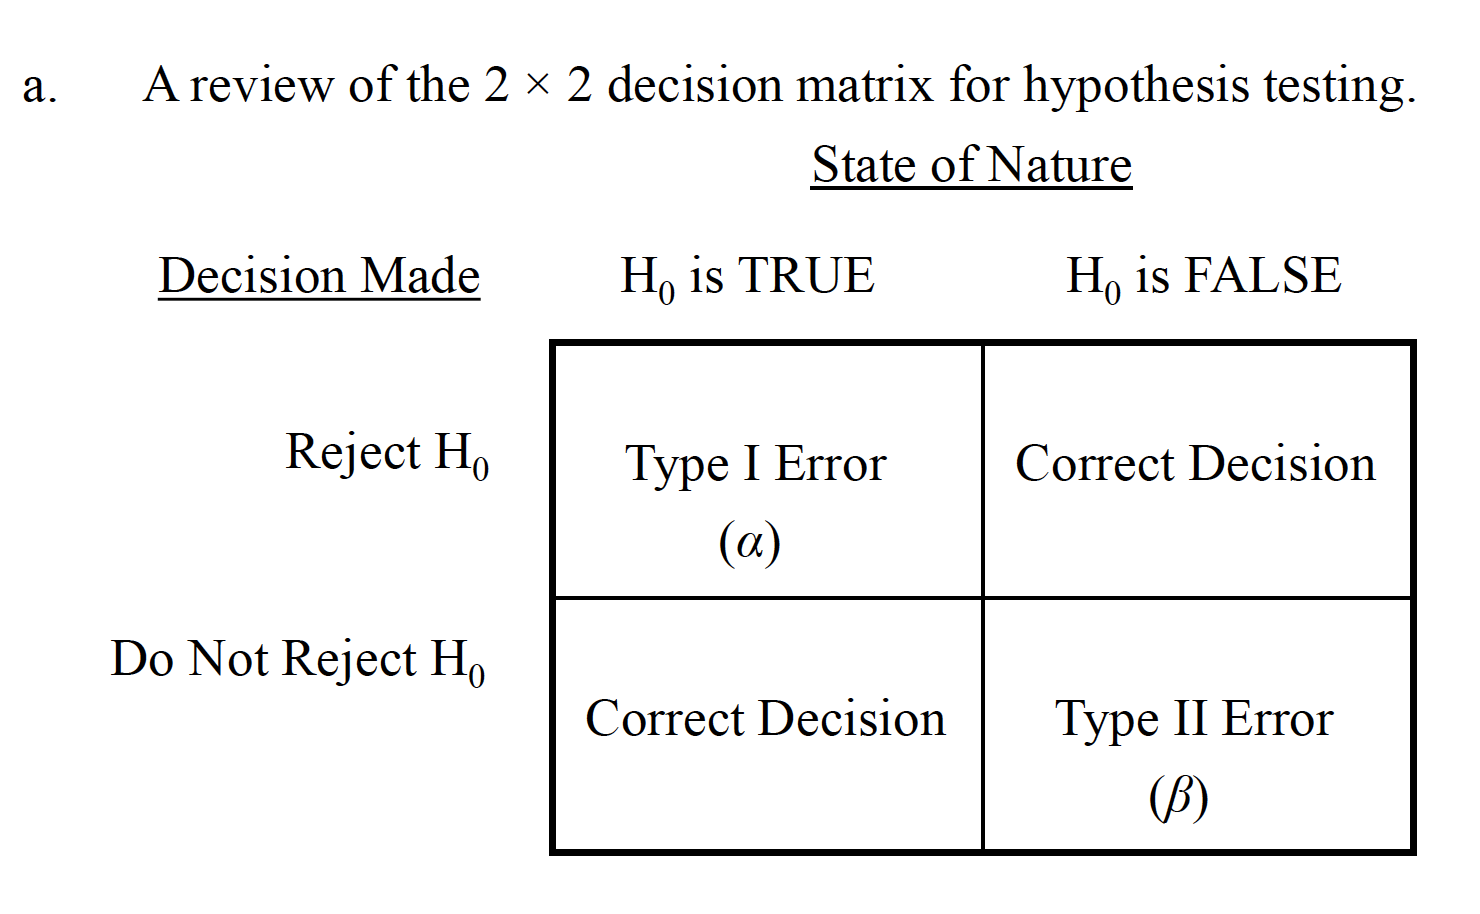
\includegraphics{img/hickspower1.png}
\caption{Table}
\end{figure}

Careful planning of research involves minimizing Type I andType II
errors. One rule of thumb is that \(\beta\) should be no more than .20
(e.g., if \(\alpha\) = .05, \(\beta\) = .20). c.For the t test, if the
null hypothesis distribution is centered on a t value of 0, then the
noncentralt distribution represents the alternative hypothesis
distribution, centered on \(\delta\). -This represents the average t
value one would expect for a given effect size and sample size

\begin{figure}
\centering
\includegraphics{img/hickspower2.png}
\caption{Noncentral T}
\end{figure}

\subsection{Test Equations}\label{test-equations}

One Sample tests

\$ \delta = d\sqrt{n}\$ \(d = \frac{\bar{X}-\mu}{\sigma}\)
\(g = \frac{\bar{X}-\mu}{s}\)

Two sample tests

\(\delta = d\sqrt{\frac{n}{2}}\) \(d = \frac{\mu_1-\mu_2}{\sigma}\)
\(g = \frac{\bar{X_1}=\bar{X_2}}{s_p}\)

For unequal n

\(n_n = \frac{2n_2n_2}{n_1 + n_2}\)
\(g = t\sqrt{\frac{n_1 + n_2}{n_1n_2}}\)

\begin{figure}
\centering
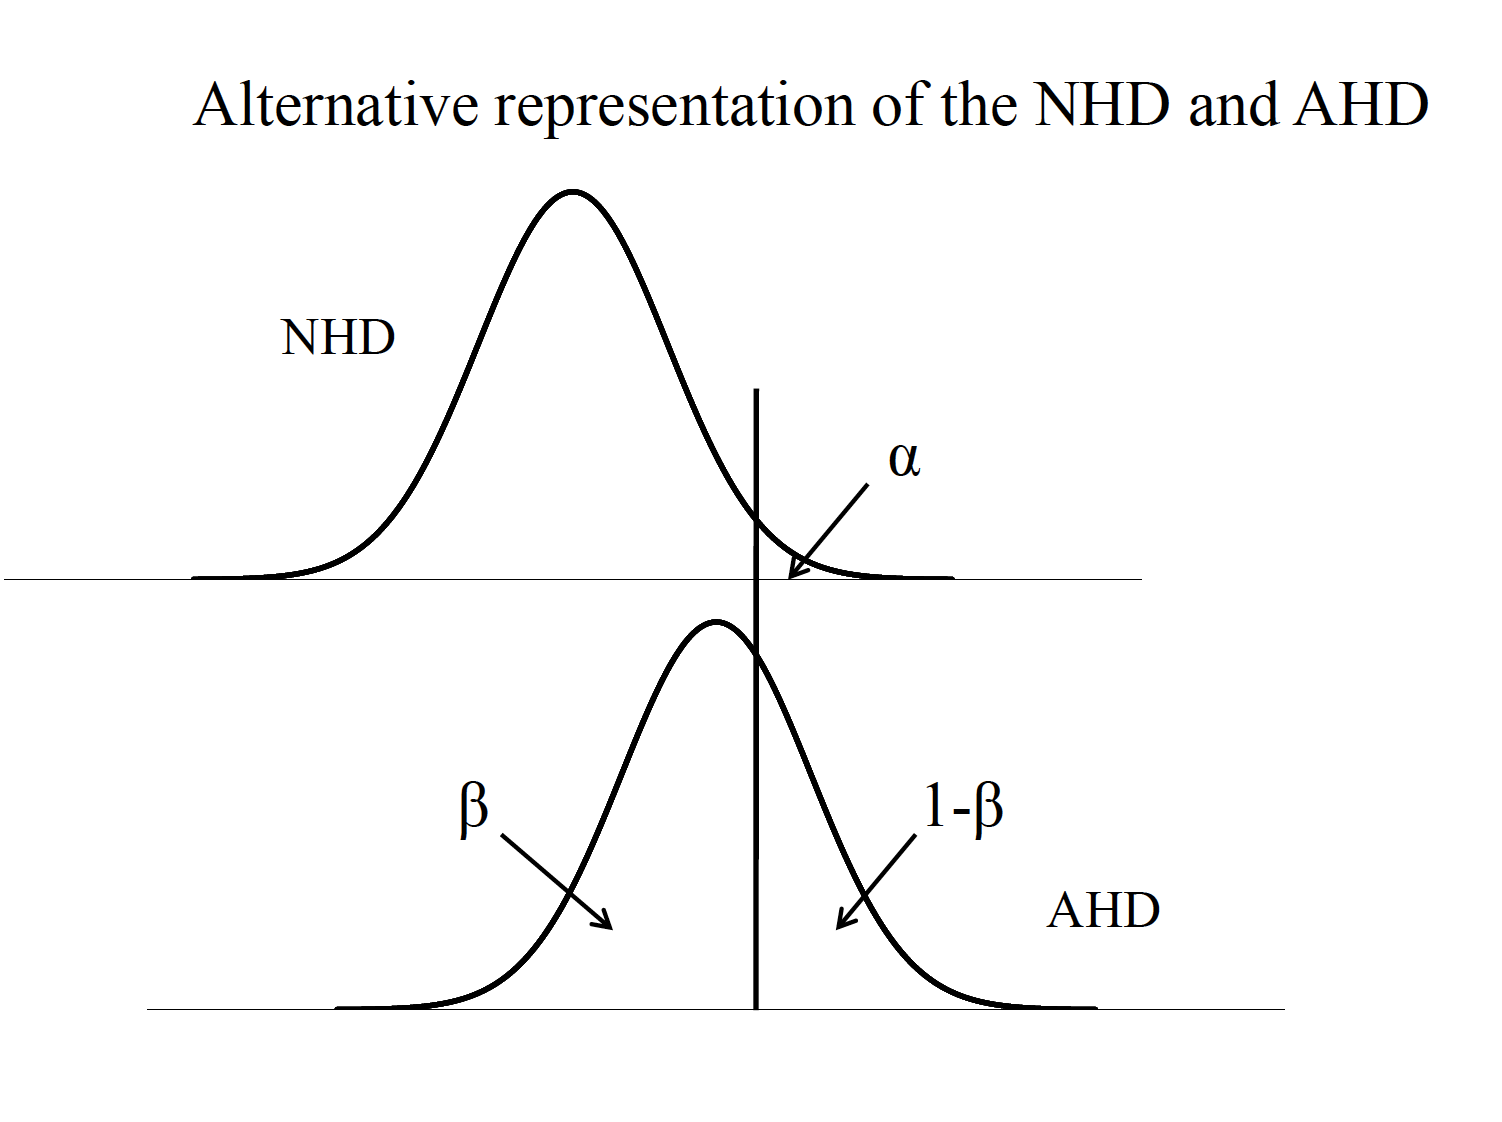
\includegraphics{img/hickspower3.png}
\caption{Noncentral T}
\end{figure}

Effect size (ES) or standardized effect size (e.g., d). i. The
difference between population means (e.g., \(\mu1-\mu2\)). ii. The
population standard deviation (\(\sigma\)).

\begin{figure}
\centering
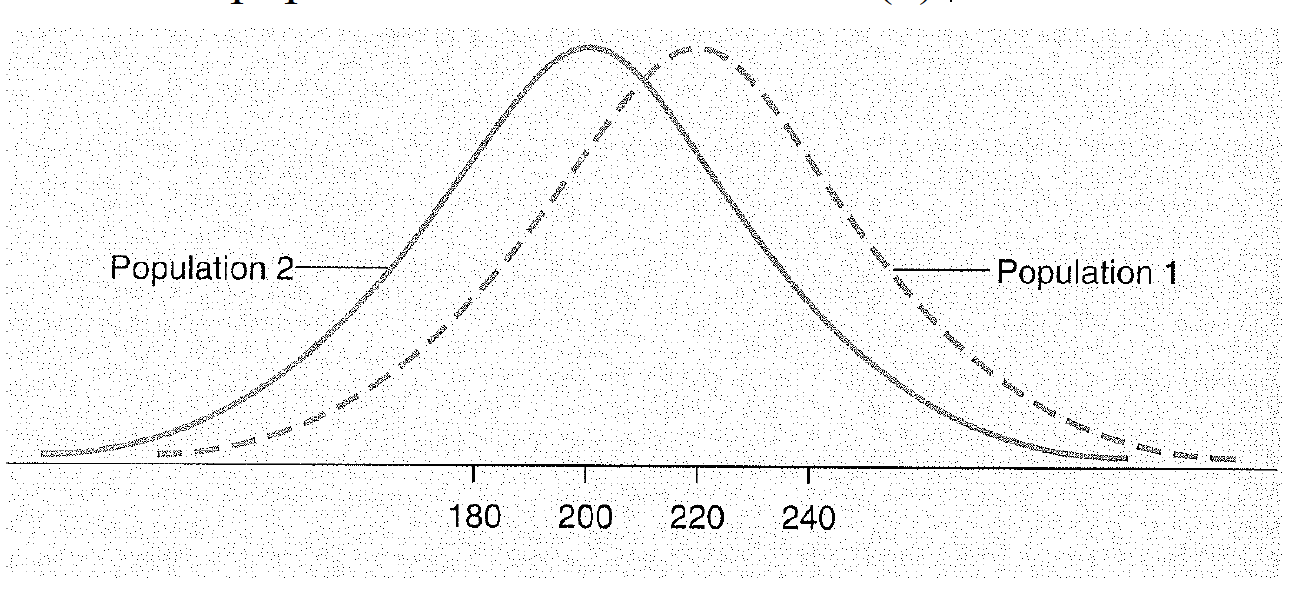
\includegraphics{img/hickspower4.png}
\caption{Noncentral T}
\end{figure}

\subsection{Factors of Power}\label{factors-of-power}

\begin{enumerate}
\def\labelenumi{\arabic{enumi}.}
\tightlist
\item
  Effect size (ES) or standardized effect size (e.g., d). \emph{The
  difference between population means (e.g., \(\mu_1-\mu_2\)). }The
  population standard deviation (\(\sigma\)).
\item
  Sample size (\(n\)).
\item
  Significance level (\(\alpha\)).
\item
  Directionality of the hypothesis test (one-tailed vs.~two-tailed).
\end{enumerate}

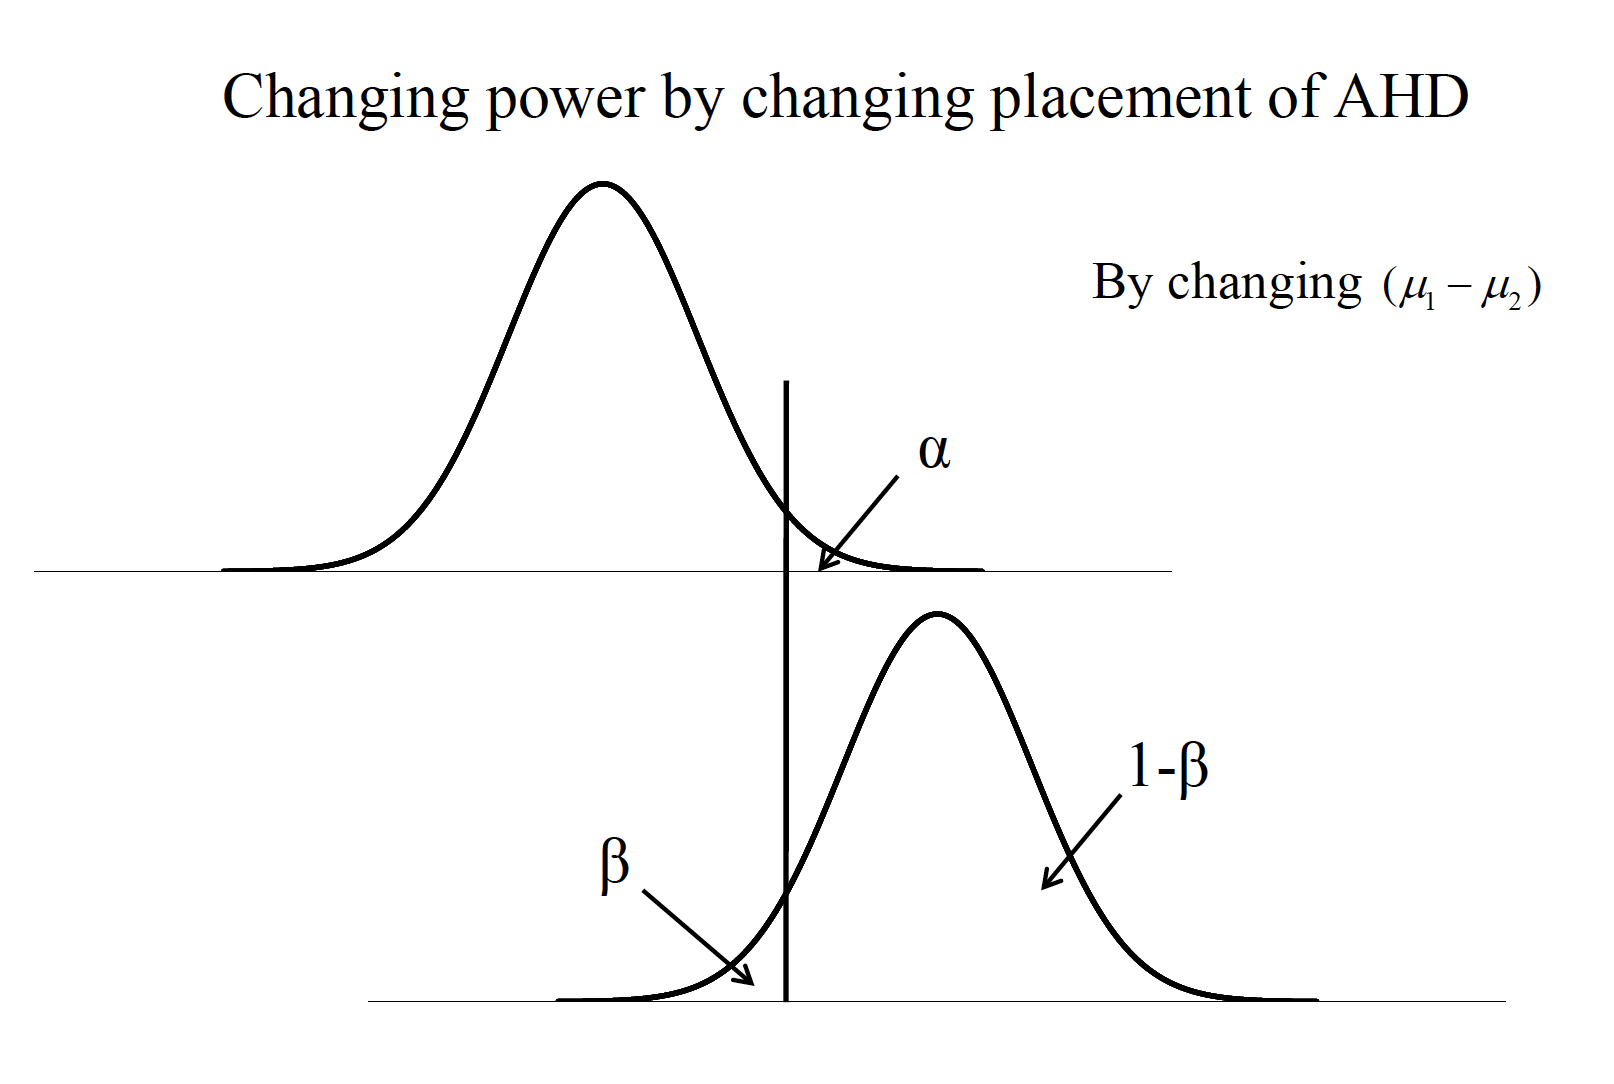
\includegraphics{img/hickspower5.png}
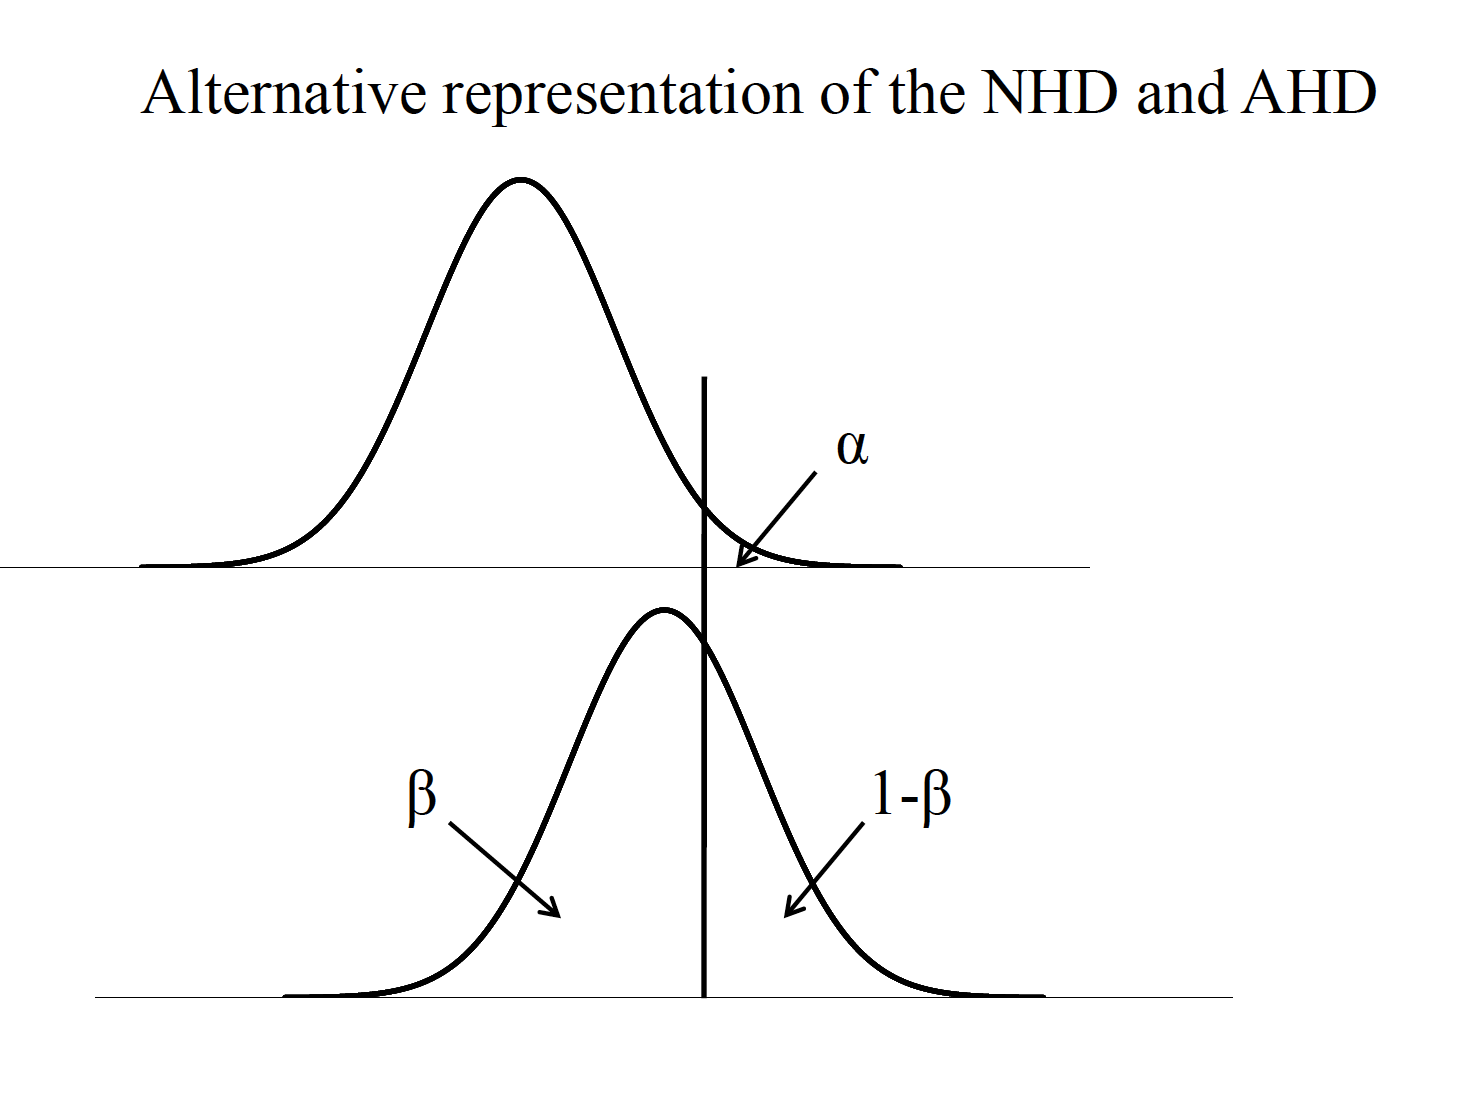
\includegraphics{img/hickspower6.png}
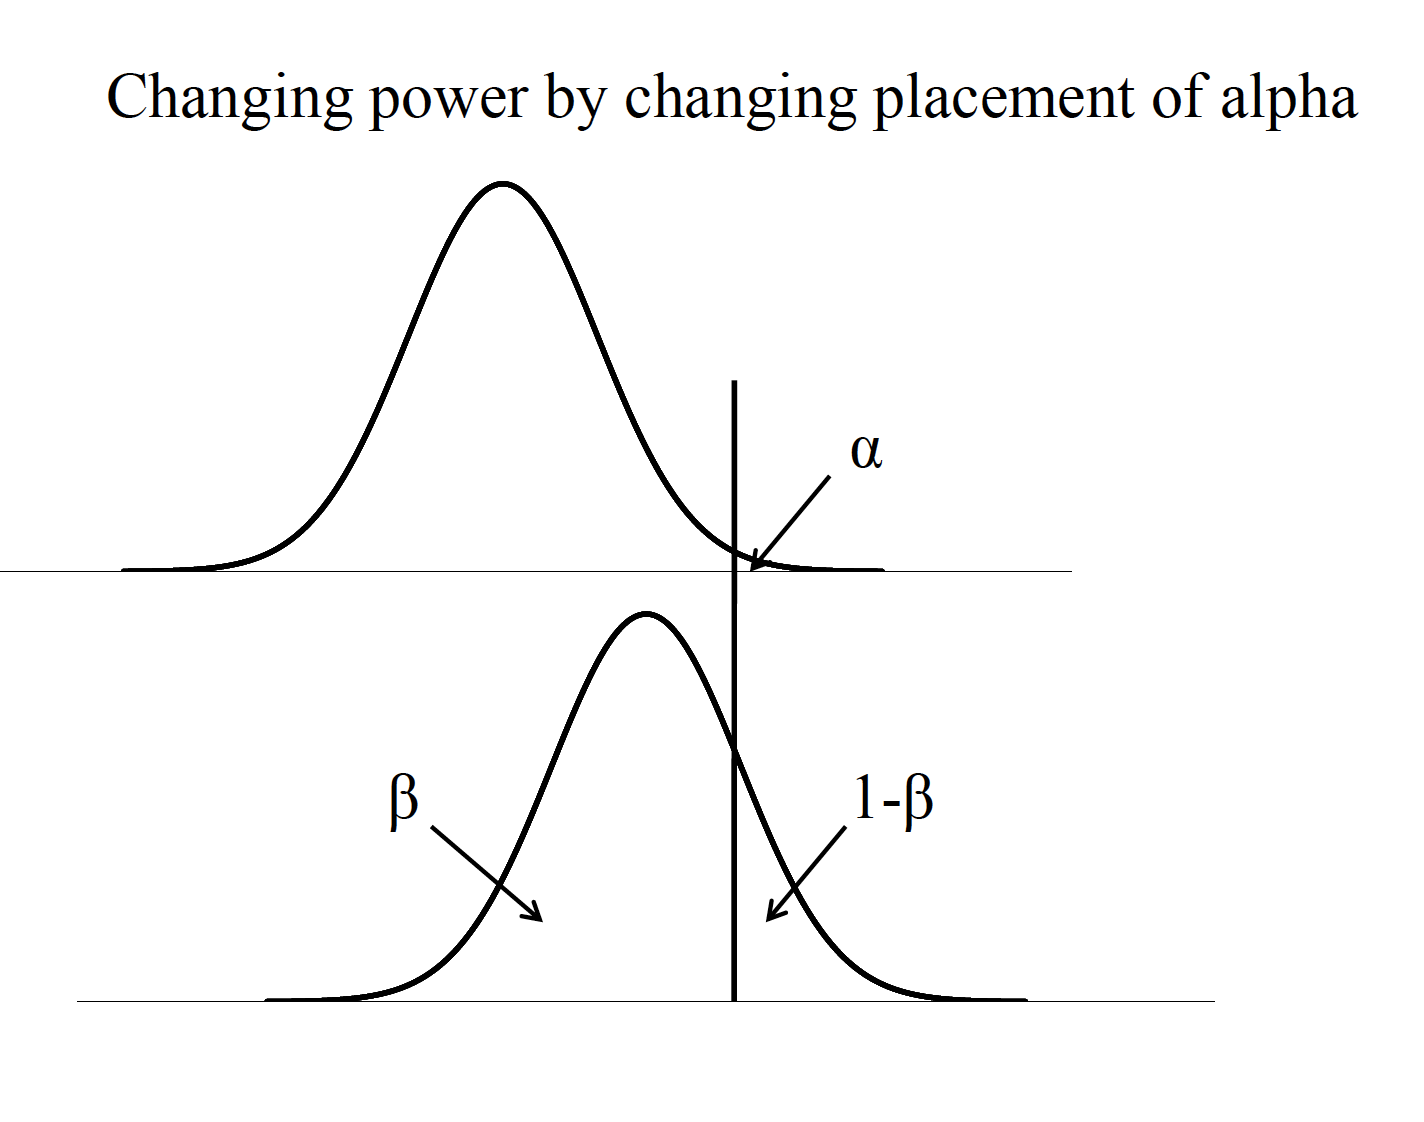
\includegraphics{img/hickspower7.png}
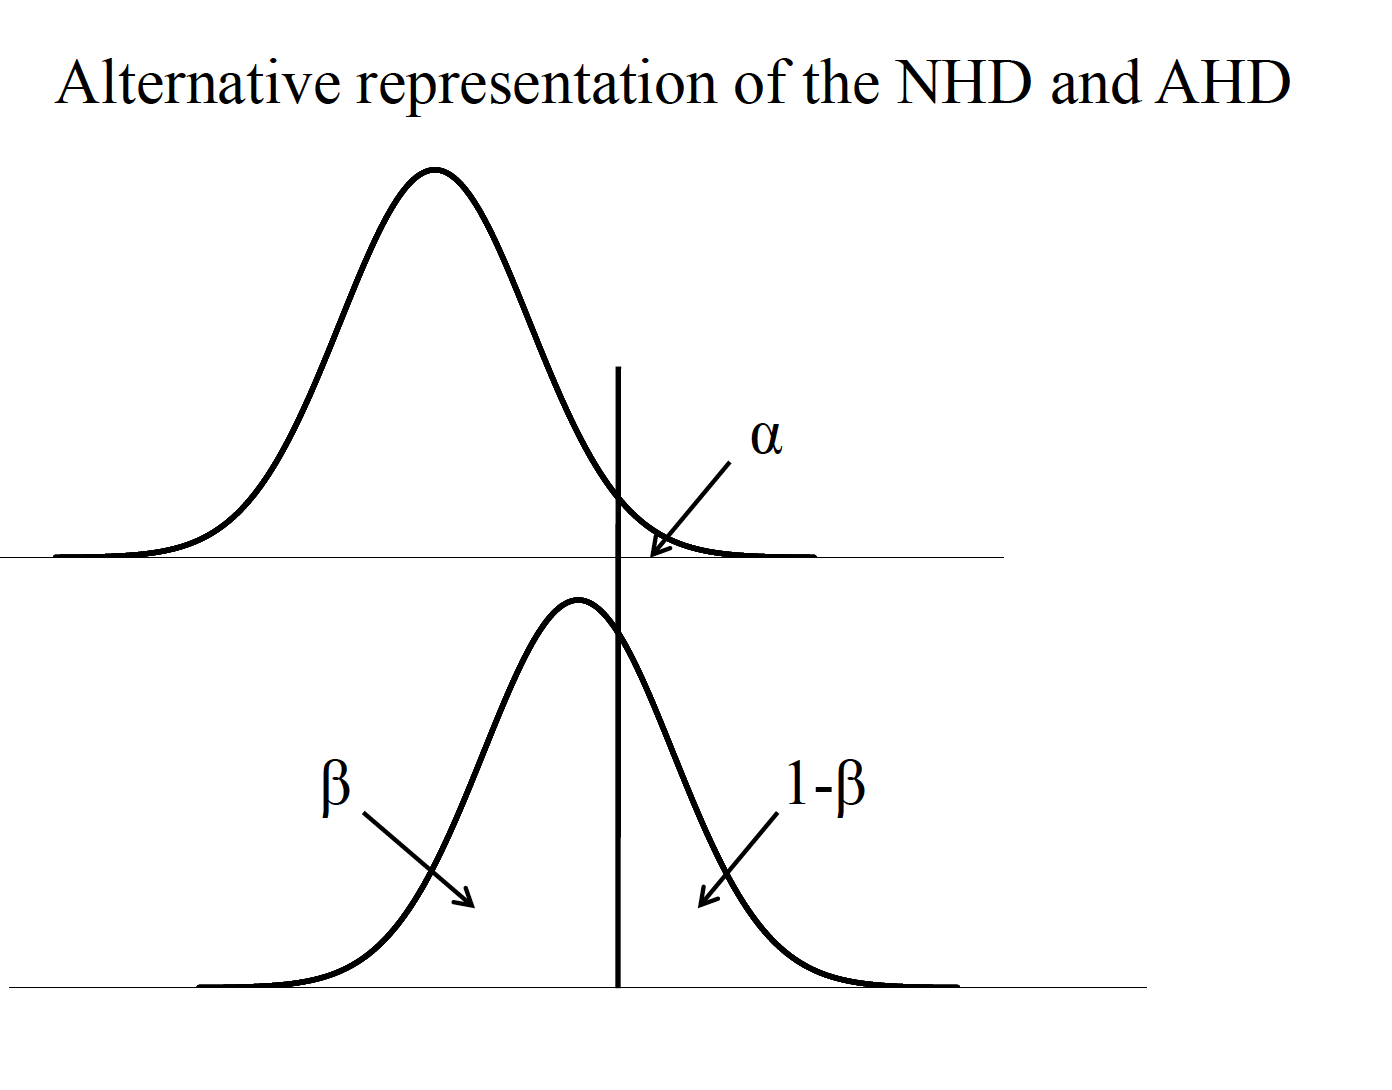
\includegraphics{img/hickspower8.png}
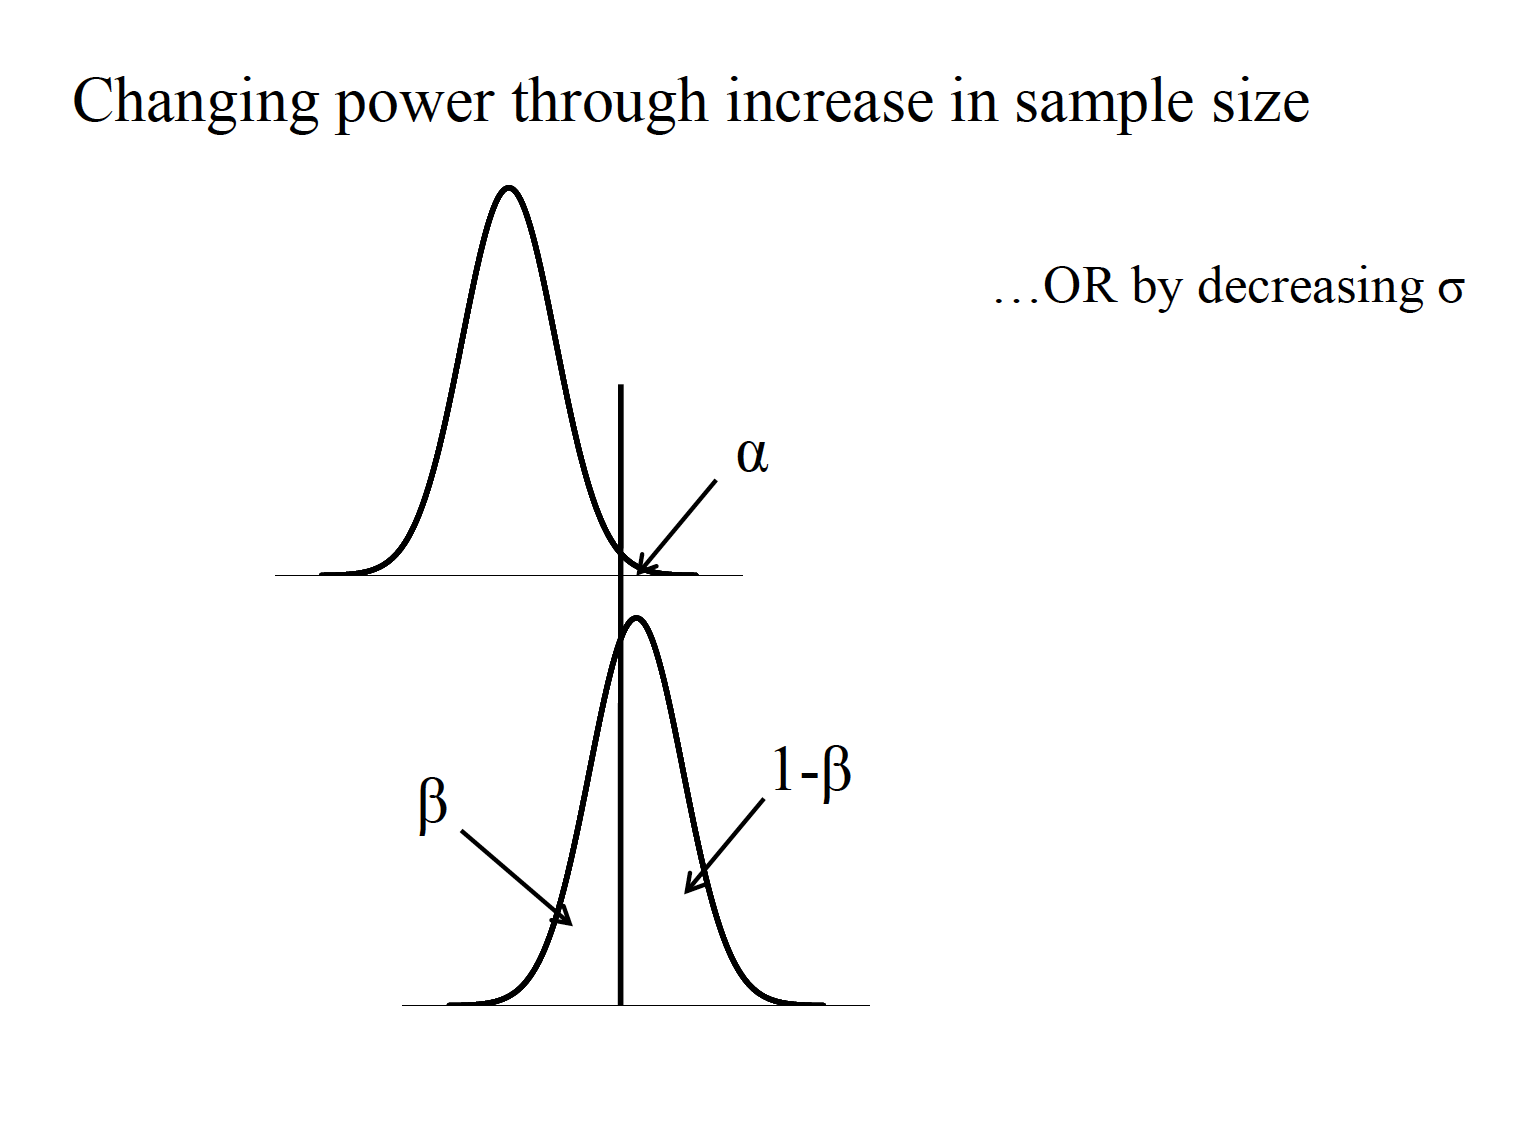
\includegraphics{img/hickspower9.png}

One sample case

\(\delta = d\sqrt{n}\) \(n = (\frac{\delta}{d})^2\)

two sample case

\(delta = d\sqrt{\frac{n}{2}}\) \(n = 2(\frac{\delta}{d})^2\)

A clinical psychologist wants to test the hypothesis that people who
seek treatment for psychological problems have higher IQs than the
general population. To test her hypothesis, she wants to use the IQ
values from 25 randomly selected clients and also to calculate the power
to find a 5-point difference in IQ. The mean of the population would be
100 and, therefore, the mean of her clients a 105. The population SD for
IQ is 15. (This scenario is from Howell's 2002 text ``Statistical
Methods for Psychology'')

Known: \(\mu_{client}=105\) \(\mu_{pop}\) \(\sigma_{pop} = 15\)

Calculate it with

\(d = \frac{105-100}{15} = 0.33\)

\(\delta = d\sqrt{n} = 0.33\sqrt{25}=1.65\)

Given this information and an expected alpha (two-tailed) of .05, we can
find in Table A.4 in the Cohen text that the power is between .25 and
.50, and more exactly about halfway in between (around .38). What does
this value of .38 mean?

If power should be at or above .80, what does the clinician do? Increase
alpha? Decrease the population SD? Increase the difference between
population means? Increase sample size? For a power level of .80, δneeds
to be 2.80, from Table A.4

\(n = (\frac{\delta}{d})^2=(\frac{2.80}{0.33}^2 = 8.48^2 = 71.91\)

\section{Confidence Ientervals}\label{confidence-ientervals}

\begin{enumerate}
\def\labelenumi{\arabic{enumi}.}
\item
  Sample measures of central tendency, such as the mean, are considered
  point estimates of population parameters. Confidence intervals are
  considered a type of interval estimation for population parameters.
\item
  Computation of confidence intervals.
\item
  Capture percentage, prediction, and replication
\end{enumerate}

Over repeated sampling from a known distribution, the confidence
interval represents the percentage of such intervals that contain the
population mean. Can be set at any percentage: 90\%, 95\%, 99\% Based on
characteristics of the sampling distribution (zor t) and therefore
highly related to the manner in which sampling distributions are used
for NHST  But CIs and pvalues from NHST are not the same thing!!!

\begin{figure}
\centering
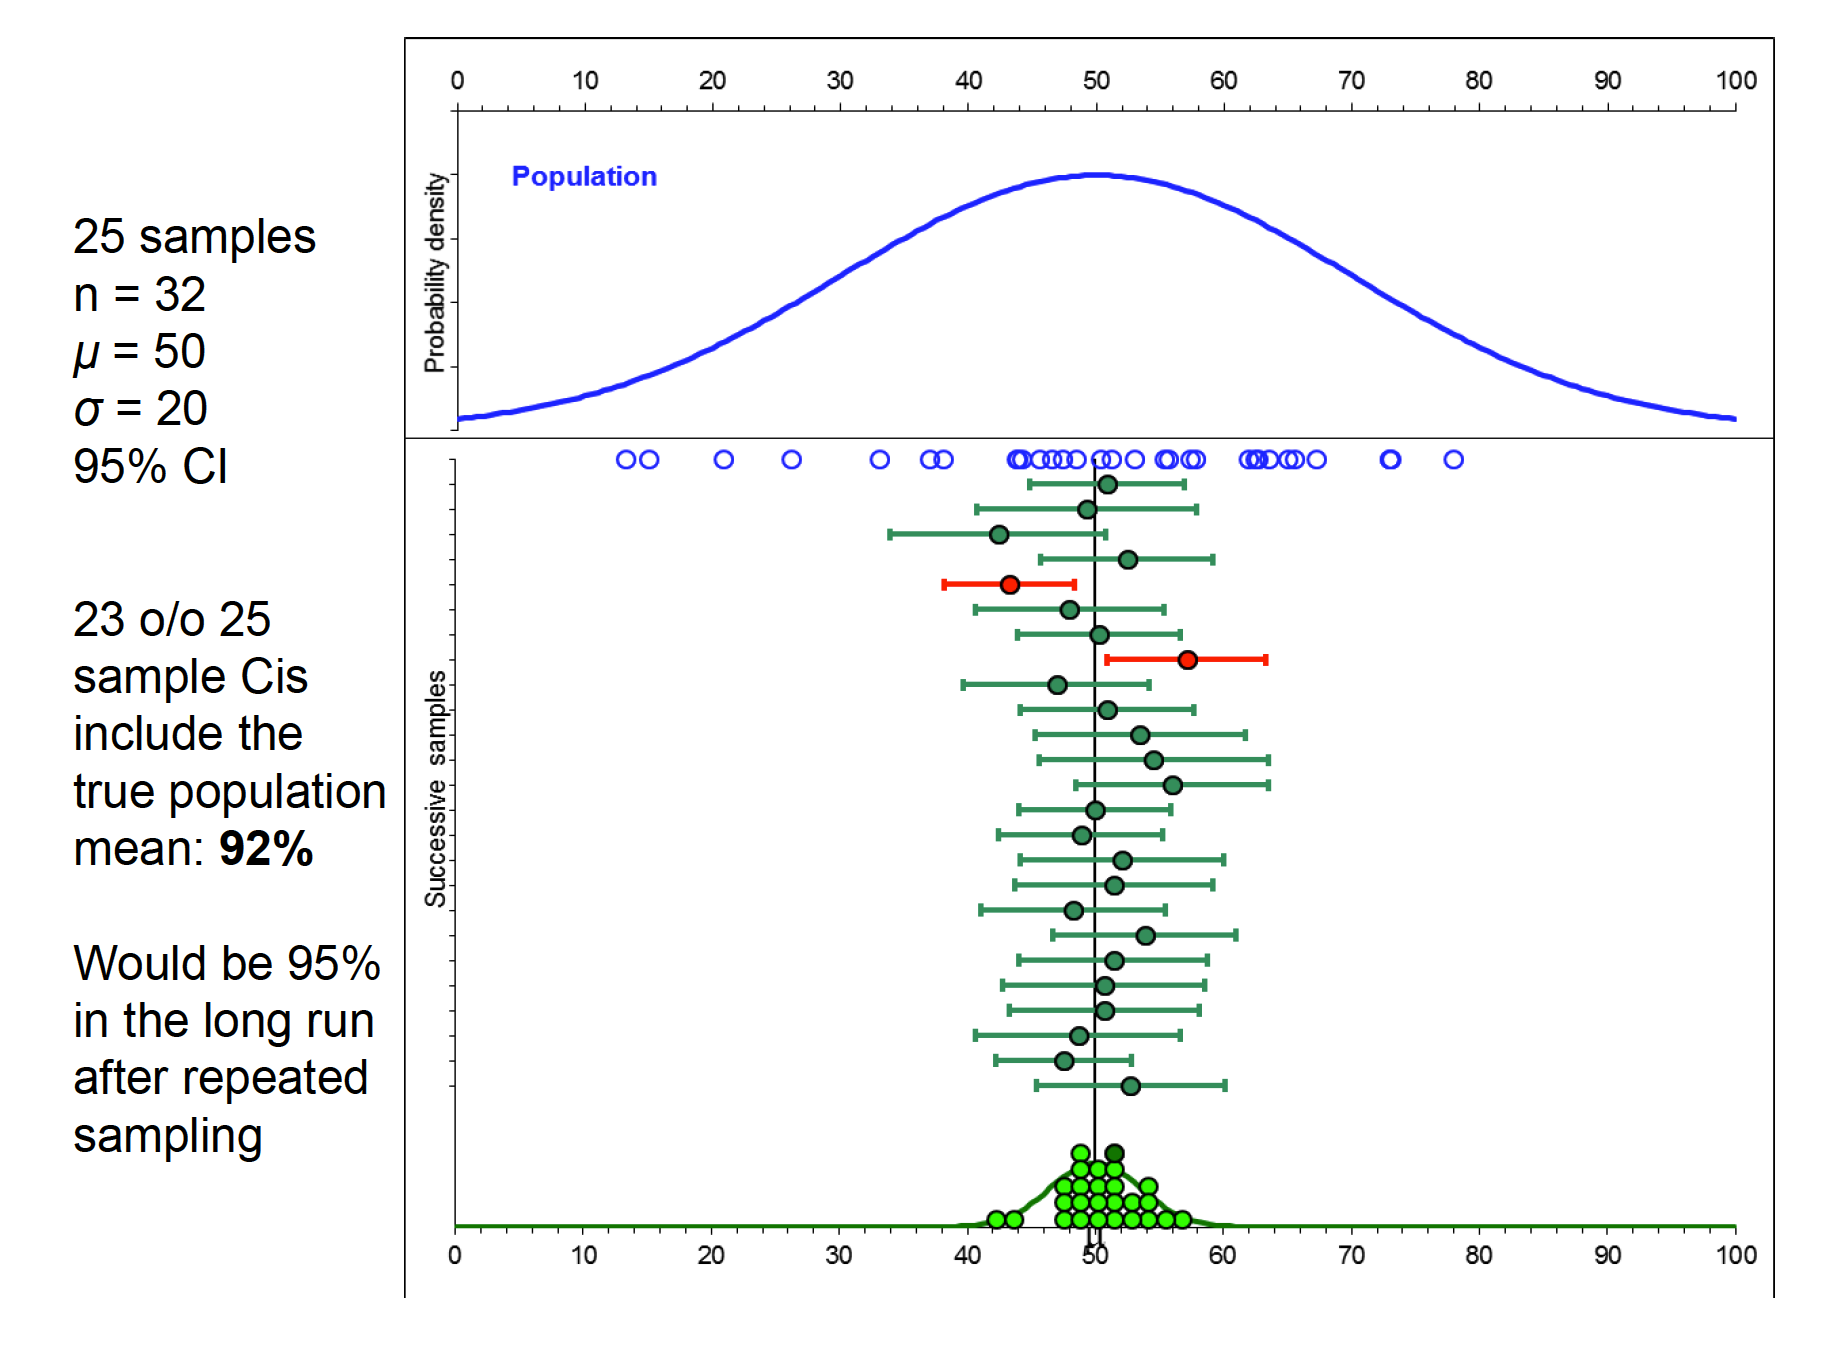
\includegraphics{img/hicksci1.png}
\caption{Hicks CI 1}
\end{figure}

Confidence Interval for single sample mean

\(\bar{X} = +- (t_{cv})s_{\bar{X}}\)

Confidence interval for a mean difference scores (dependent samples)

\(\bar{D} +- (t_{cv})s_{\bar{D}\)

Confidence interval for a difference between sample means (independent
samples)

\((\bar{X_1}-\bar{X_2}) +- (t_{cv})(s_{\bar{X_1}-\bar{X_2}})\)

The instructor of an introductory psychology course is interested in
knowing if there is a difference in the mean grades on the final exam
between the fall and spring semester classes. Summary data for the two
samples is below:

What are the 95\% confidence intervals around each sample mean, and
around the difference between the sample means?

\begin{Shaded}
\begin{Highlighting}[]
\NormalTok{fall <-}\StringTok{ }\KeywordTok{c}\NormalTok{(}\FloatTok{82.4}\NormalTok{,}\DecValTok{150}\NormalTok{,}\FloatTok{11.56}\NormalTok{)}
\NormalTok{spring <-}\StringTok{ }\KeywordTok{c}\NormalTok{(}\FloatTok{84.2}\NormalTok{,}\DecValTok{150}\NormalTok{,}\FloatTok{11.44}\NormalTok{)}
\NormalTok{stat <-}\StringTok{ }\KeywordTok{c}\NormalTok{(}\StringTok{"Mean"}\NormalTok{,}\StringTok{"N"}\NormalTok{,}\StringTok{"s2"}\NormalTok{)}
\NormalTok{grades <-}\StringTok{ }\KeywordTok{data.frame}\NormalTok{(stat,fall, spring)}
\NormalTok{grades}
\end{Highlighting}
\end{Shaded}

\begin{verbatim}
##   stat   fall spring
## 1 Mean  82.40  84.20
## 2    N 150.00 150.00
## 3   s2  11.56  11.44
\end{verbatim}

What are the 95\% confidence intervals around each sample mean, and
around the difference between the sample means?

Confidence Interval for single sample mean

\(\bar{X} = +- (t_{cv})s_{\bar{X}}\)

This has critical value of 1.97 +-.

First need to find the standard error with each one.

\$s\_\bar\{X\} = \frac{s}{\sqrt{n}} = \frac{\sqrt{11.56}}{\sqrt{150}} =
\frac{3.4}{12.25}= 0.28 \$

\$s\_\bar\{X\} = \frac{s}{\sqrt{n}} = \frac{\sqrt{11.44}}{\sqrt{150}} =
\frac{3.4}{12.25}= 0.28 \$

Now do CI for both

\(\bar{X} = +- (t_{cv})s_{\bar{X}}\)

\(82.4 +- (1.97)(0.28)\) \(82.4 +- 0.55\) \((81.85, 82.95)\)

\(84.2 +- (1.97)(0.28)\) \(84.4 +- 0.55\) \((83.65, 84.75)\)

Calculate that now for differences

\((\bar{X_1}-\bar{X_2}) +- (t_{cv})(s_{\bar{X_1}-\bar{X_2}})\)

\(s_{\bar{X_1}-\bar{X_2}}= \sqrt{0.07 + 0.07} = \sqrt{0.14}=0.37\)

Alpha value associated with this is 1.96.

\(82.4 - 84.2) +- (1.96)(0.37)\) \(-1.8 +- 0.73 = (-2.53,-1.07)\)

Important points to keep in mind regarding confidence intervals:

\begin{enumerate}
\def\labelenumi{\arabic{enumi}.}
\tightlist
\item
  They are two-tailed by nature (i.e., on either side of a sample mean).
\item
  For a given sample size, increasing the level of confidence (e.g.,
  from 95\% to 99\%) increases the interval width.
\item
  The narrower the interval (at a given level of confidence!) reflects
  better statistical precision. Sample size directly affects the width
  of the interval by affecting the standard error estimate.
\end{enumerate}

\subsection{Capture Percentage}\label{capture-percentage}

Capture percentage, prediction, and replication What is the likelihood
that a subsequent experiment will replicate? Concept of capture
percentage: likelihood that a subsequent sample mean will fall into the
CI of the current sample.

\begin{figure}
\centering
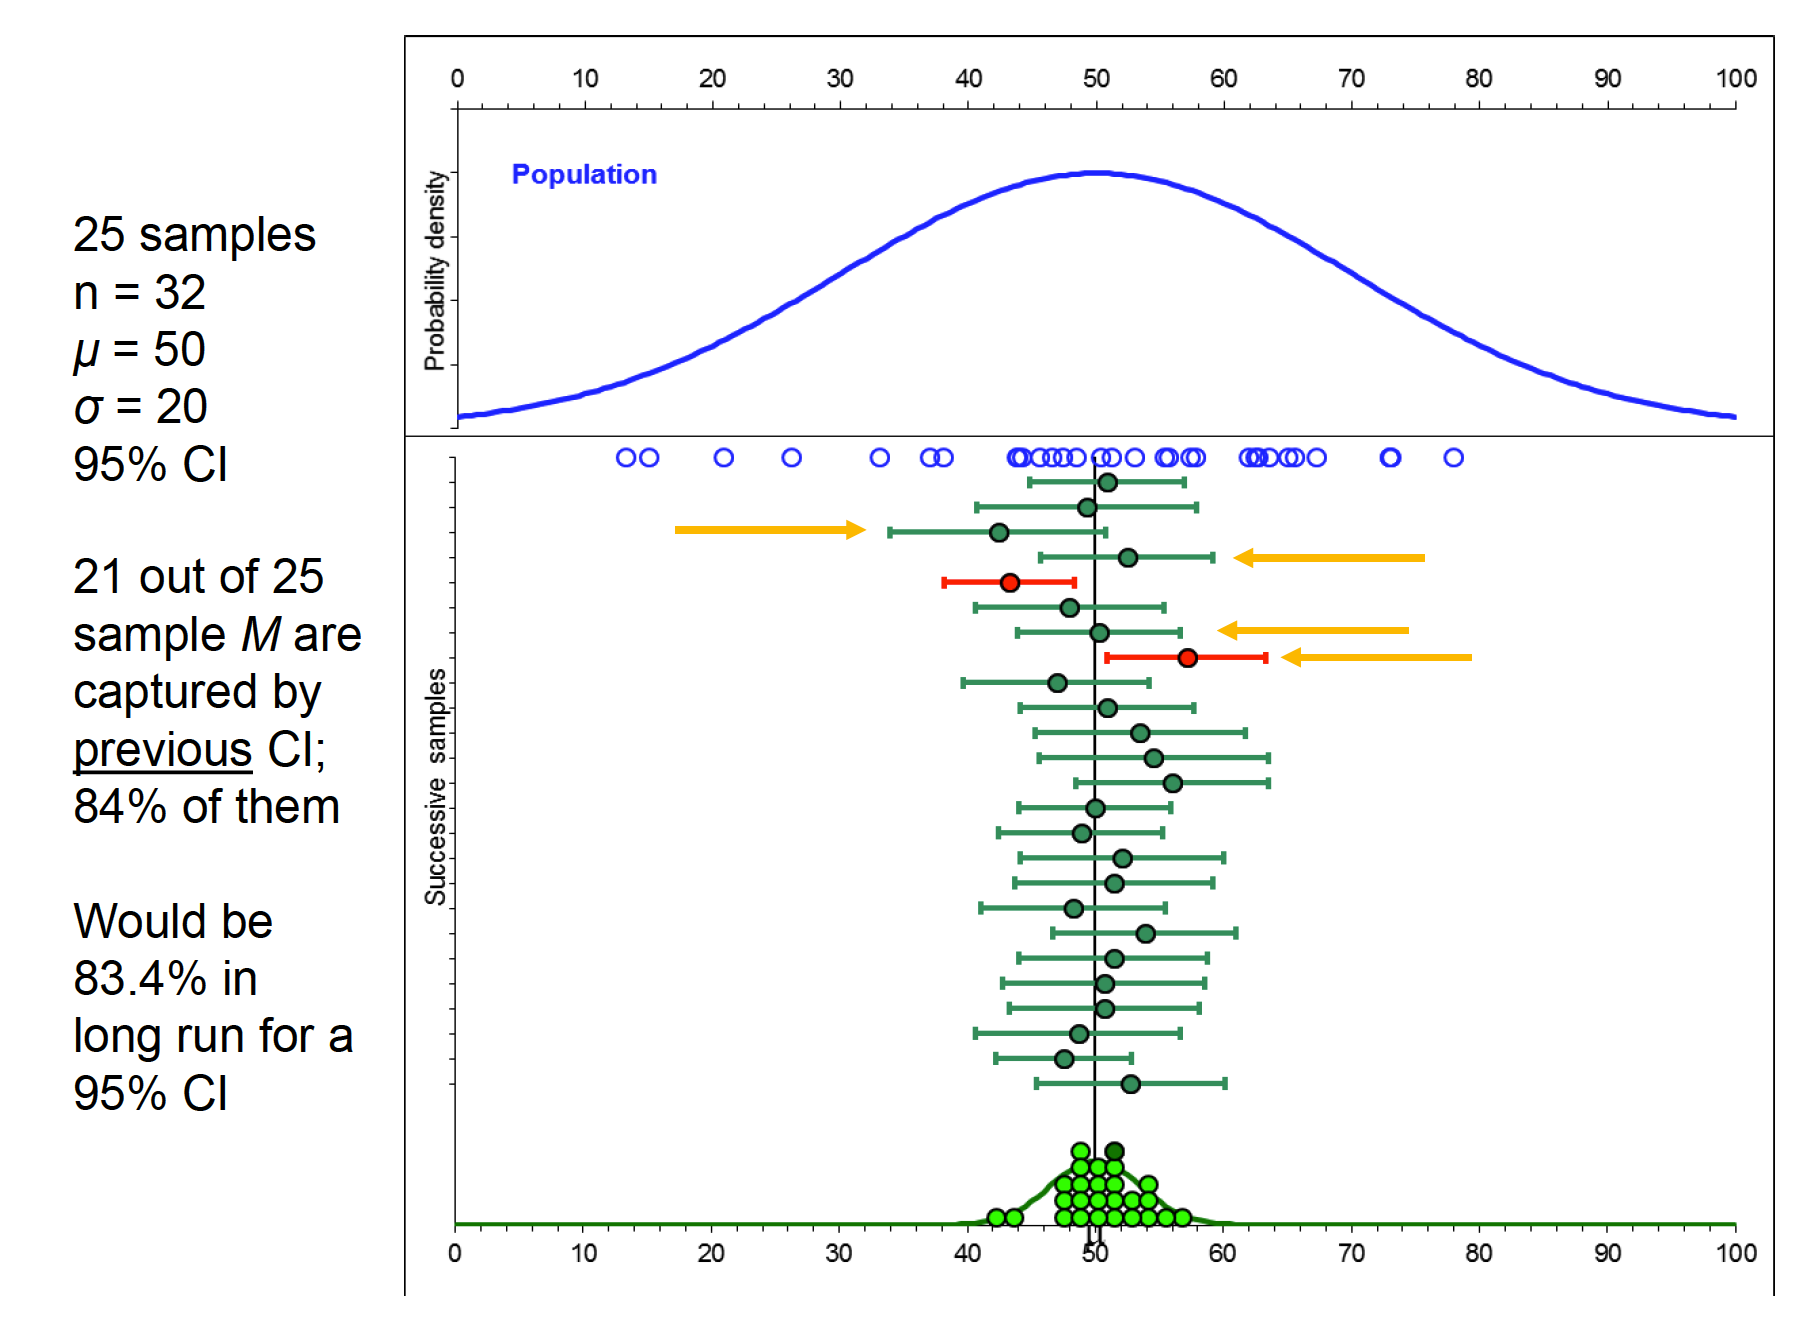
\includegraphics{img/hicksci2.png}
\caption{Hicks CI 2}
\end{figure}

\chapter{Correlation and Regression}\label{correlation-and-regression}

attempt here

\chapter{Matched T Test}\label{matched-t-test}

\section{Theory}\label{theory}

When both sample means were produced by the same participants, we
conduct what is known as a dependent-samplestest. This is a test of the
average difference between the scores in one condition and the scores in
another condition---thus, the unit of measurement is a difference score.

\(\bar{D}=\Sigma D /n\) \(D= X_{i1} - X_{i2}\)

The mean of this sampling distribution is \(\delta\)= 0. The shape of
this sampling distribution is approximately normal. The standard error
of the sampling distribution of mean difference scores is

\(s_{\bar{D}} = \frac{s_D}{\sqrt{n}}\)

\(s_d = \sqrt{\frac{\Sigma{(D-\bar{D})^2}}{n-1}}\)

The test statistic is

\(t = \frac{\bar{D}-\delta}{s_{\bar{D}}}\)
\(s_\bar{D} =\frac{s_D}{\sqrt{n}}\)

The effect size is calculated

\(d =\frac{\bar{D}}{S_D}\)

\(S_d = \sqrt{\frac{\Sigma{(D-\bar{D})^2}}{n-1}}\)

You are investigating whether the older or younger male in a pair of
brothers tends to be more extroverted. So you test where each one falls
on an introversion-extroversion scale. The results are as follows:

\begin{Shaded}
\begin{Highlighting}[]
\CommentTok{# Dep}
\NormalTok{younger <-}\StringTok{ }\KeywordTok{c}\NormalTok{(}\DecValTok{10}\NormalTok{,}\DecValTok{11}\NormalTok{,}\DecValTok{18}\NormalTok{,}\DecValTok{12}\NormalTok{, }\DecValTok{15}\NormalTok{)}
\NormalTok{older <-}\StringTok{ }\KeywordTok{c}\NormalTok{(}\DecValTok{18}\NormalTok{,}\DecValTok{17}\NormalTok{,}\DecValTok{19}\NormalTok{,}\DecValTok{16}\NormalTok{,}\DecValTok{15}\NormalTok{)}
\NormalTok{dep <-}\StringTok{ }\KeywordTok{data.frame}\NormalTok{(younger, older)}
\end{Highlighting}
\end{Shaded}

Step one: State the null and alternative hypotheses

\(H_o : \delta = \mu_1 - \mu_2 = 0\)
\(H_a : \delta = \mu_1 - \mu_2 != 0\)

Step two: Set the criterion for rejecting H0. Alpha is usually set to
.05, but could be other values depending on the research context. Make
sure you've considered directionality!

Step three: Select the sample and collect your data.

Step four: Locate the region of rejection and critical values.

\(t_{cv,dv=4, \alpha=.05}= +/- 2.77\)

Step five: Compute the appropriate statistic. We were never given
\(\sigma\)or \(\sigma^2\), so we use the t test.

\begin{figure}
\centering
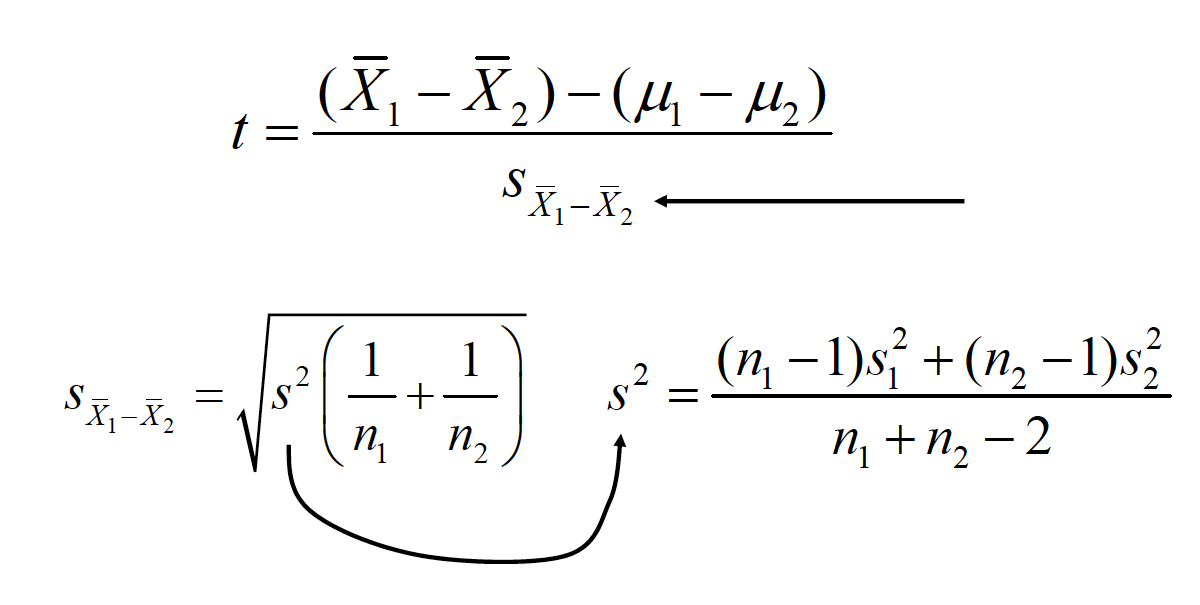
\includegraphics{img/hickssampling14.png}
\caption{Convert me}
\end{figure}

\begin{figure}
\centering
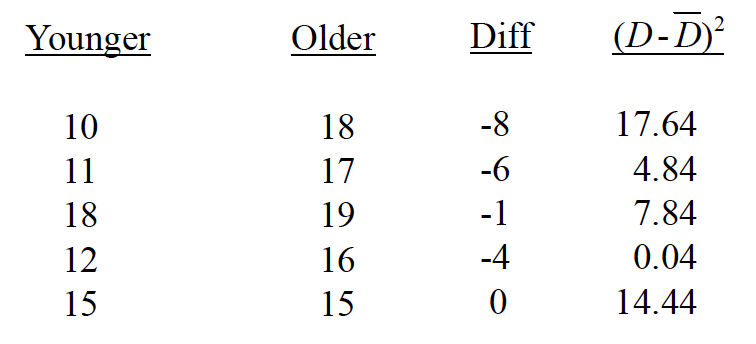
\includegraphics{img/hickssampling21.png}
\caption{Convert me}
\end{figure}

\begin{figure}
\centering
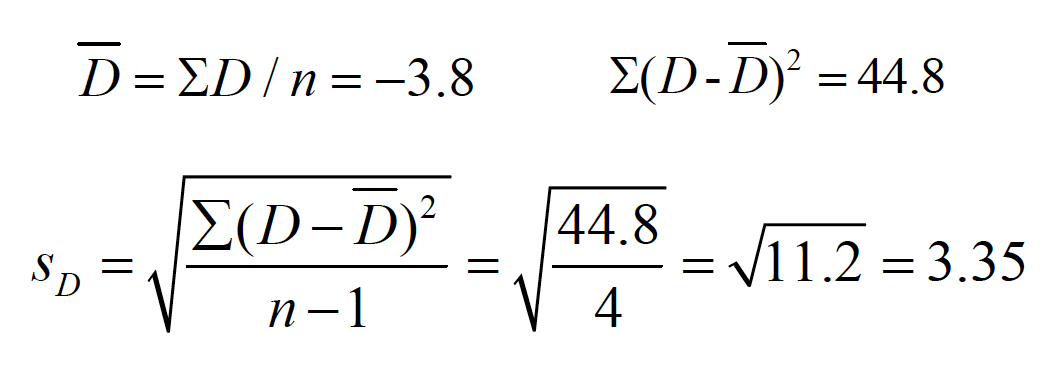
\includegraphics{img/hickssampling22.png}
\caption{Convert me}
\end{figure}

\(s_D=3.55\) \(s_\bar{D} =\frac{s_D}{\sqrt{n}}= \frac{3.35}{\sqrt{5}}\)

\(t = \frac{\bar{D}-\delta}{s_\bar{D}} = \frac{-3.8-0}{1.50}= -2.53\)

Step six: Decide whether to reject H0. Is -2.53 more extreme than the
critical value?

\(t_{cv,dv=4, \alpha=.05}= +/- 2.77\)

``The average extroversion value for the younger male siblings (M= 13.2)
did not differ significantly from the extroversion value for the older
siblings (M= 17.0), t(4) = 2.53, p\textgreater{} .05.''

Effect size computation

\(d = \frac{\bar{D}}{s_D}= \frac{-3.8}{3.35} = -1.13\)

Small: = 0.25Medium: = 0.50Large: = 1.0

``The average extroversion value for the younger male siblings (M= 13.2)
did not differ significantly from the extroversion value for the older
siblings (M= 17.0), t(4) = 2.53, p\textgreater{} .05, Cohen's d= 1.13.''

So, why does the effect size calculation disagree with the result of the
hypothesis test?

Template file

\chapter{One Way ANOVA}\label{one-way-anova}

Template file

\chapter{Multiple Comparisons}\label{multiple-comparisons}

Template file

\chapter{Simple Effects, Interactions, Mixed
Designs}\label{simple-effects-interactions-mixed-designs}

Template file

\chapter{Repeated Measures ANOVA:}\label{repeated-measures-anova}

Template file

\chapter{Mixed Two Way ANOVA}\label{mixed-two-way-anova}

Template file

\chapter{Multiple Regression}\label{multiple-regression}

Template file

\chapter{Chi-Square}\label{chi-square}

Template file

\chapter{Non-Parametric Data}\label{non-parametric-data}

Template file

\chapter{Advanced Data Cleaning}\label{advanced-data-cleaning}

Template file

\chapter{Advanced Multiple
Regression}\label{advanced-multiple-regression}

Template file

\chapter{Logistic Regression}\label{logistic-regression}

Template file

\chapter{Mediation and Moderation}\label{mediation-and-moderation}

Template file

\chapter{ANCOVA}\label{ancova}

\section{Theory}\label{theory-1}

\subsection{Reducing Noise}\label{reducing-noise}

Just like the ANOVA (Analysis of Variance), the ANCOVA (Analysis of
Covariance) is used to analyze experiments by calculating an F ratio for
more than 2 groups. As with any F calculation, differences in the
dependent variable are caused by two things:

\begin{enumerate}
\def\labelenumi{\arabic{enumi}.}
\tightlist
\item
  The independent variable (signal, systematic variation)
\item
  Error (noise, unsysematic variation)
\end{enumerate}

The F statistic captures this

\[ F = \frac{Variation\ Due\ to\ IV}{Variation\ Due\ to\ Error} \]

When there is small variation within groups and large variation between
groups, we get a large F.

CHART HERE

When there is large variatin within groups and small variation between
groups, we get a small F.

The idea with the ANCOVA is that you can reduce your error term (the
denominator from above) by choosing a covariate (CV) that is related to
the DV and will soak up some random variation in your F test to give you
a clearer picture of what is going on. Usually this means controlling
for some sort of variable. The classic example is if you wanted to give
some kids a test of some mental ability in a between subjects design but
you don't want their age to skew your results. You might have had a
control condition, an intervention, and some sort of alternate
intervention. Typically you would run an ANOVA on the three groups, but
since you know age has been accounted for and you want to remove that
effect from the model, you enter age as a covariate in this calculation.
Outside of this there are \textbf{three} major applications for ANCOVA.

\begin{enumerate}
\def\labelenumi{\arabic{enumi}.}
\tightlist
\item
  Increase test sensitivity by using the CV(s) to account for more of
  the error variance
\item
  Adjust DV scores to what they would be if everyone scored the same on
  the CV(s)
\item
  Adjustment of a DV for other DVs taken as CVs
\end{enumerate}

Note that use of a CV can adjust DV scores and show a larger effect or
the CV can even eliminate the effect. Looking at this another way:

\begin{enumerate}
\def\labelenumi{\arabic{enumi}.}
\tightlist
\item
  Reduces random error by increasing the size of F
\item
  Reduces systematic error by adjusting for differences in means
\item
  May increase differences by soaking up error
\end{enumerate}

It's a \textbf{good} idea to use ANCOVA when you are removing variance
in the DV related to covariate, but not related to the grouping
variable. This decreases the error term and increases power.

It'sa \textbf{bad} idea to use ANCOVA when groups differ on their mean
level of the covariate. Usually here the covariate and the grouping
variable are not independent. An example of this might be when
``controlling'' for anxiety when studying people with and without
depression. Clearly people with depression will have higher levels of
anxiety than their controls by nature of having depression!

\subsection{Assumptions of ANOVA}\label{assumptions-of-anova}

\begin{enumerate}
\def\labelenumi{\arabic{enumi}.}
\tightlist
\item
  All ANOVA assumptions apply (errors are RIND)
\end{enumerate}

\begin{itemize}
\tightlist
\item
  Random
\item
  Independent
\item
  Normally distributed
\end{itemize}

\begin{enumerate}
\def\labelenumi{\arabic{enumi}.}
\setcounter{enumi}{1}
\tightlist
\item
  The Covariate z is unrelated to x, and that z is related to, and in a
  sense, acts as a suppressor of y
\item
  The covariate has a \textbf{linear} relationship with the dependent
  variable
\item
  Variance of groups are equal.
\item
  Correlation between y and z is equal for all levels of x (Homogeneity
  of Regression)
\end{enumerate}

You test for homogeneity of regression slopes by including a covariate
by group interaction. If it's significant, you violated an assumption
and can't to ANCOVA!

CHART

CHART

\subsection{Best Practice}\label{best-practice}

Things you should control for: 1. Broad Descriptors (Age, Social Class)
2. General Ability (intellgience, memory, speed of movement) 3.
Personality measures (extraversion, neuroticism) 4. Things you think are
relevant 5. Pick CVs that are correlated with DV * Height good for
basketball * Height poor for test of math skills 6. CV should not be
influenced by treatment

\section{Practice}\label{practice-1}

In order to get our hands dirty with ANCOVA we're going to look at a
dataset where a bunch of sheep were slaughtered. We have three types of
sheep (ewe, wether, ram) and a measure of fatness and weight.

Let's first run an ANOVA to see if fatness differs between animal type.

\begin{Shaded}
\begin{Highlighting}[]
\KeywordTok{library}\NormalTok{(data.table)}
\end{Highlighting}
\end{Shaded}

\begin{verbatim}
## Warning: package 'data.table' was built under R version 3.4.2
\end{verbatim}

\begin{Shaded}
\begin{Highlighting}[]
\NormalTok{deadsheep <-}\StringTok{ }\KeywordTok{fread}\NormalTok{(}\StringTok{"datasets/deadsheep.csv"}\NormalTok{)}
\NormalTok{deadsheep[, Animal }\OperatorTok{:}\ErrorTok{=}\StringTok{ }\KeywordTok{as.factor}\NormalTok{(animal)]}
\NormalTok{sheep.model.}\DecValTok{1}\NormalTok{ <-}\StringTok{ }\KeywordTok{aov}\NormalTok{(fatness }\OperatorTok{~}\StringTok{ }\NormalTok{Animal, }\DataTypeTok{data=}\NormalTok{deadsheep)}
\KeywordTok{summary}\NormalTok{(sheep.model.}\DecValTok{1}\NormalTok{)}
\end{Highlighting}
\end{Shaded}

\begin{verbatim}
##             Df Sum Sq Mean Sq F value Pr(>F)  
## Animal       2  124.4   62.21   3.165 0.0566 .
## Residuals   30  589.6   19.65                 
## ---
## Signif. codes:  0 '***' 0.001 '**' 0.01 '*' 0.05 '.' 0.1 ' ' 1
\end{verbatim}

Looking at the output, we note that There was no significant effect of
fatness on levels of animal, \[F(2,30)=3.165, p > .05\].

Now since we know that the whole weight of the animal might be
confounding our answer (it's related to the DV of fatness, but not
nessecarily related to the type of sheep), let's run an ANCOVA with
carcass weight as a covariate and see if that changes our answer.

Before we run the ANCOVA, we need to first check that our IV is not
significantly related to our CV. We do this by running an ANOVA
predicting weigth by animal.

\begin{Shaded}
\begin{Highlighting}[]
\CommentTok{#Test IND of IV and CV}
\NormalTok{ind.sheep <-}\StringTok{ }\KeywordTok{aov}\NormalTok{(weight }\OperatorTok{~}\StringTok{ }\NormalTok{Animal, }\DataTypeTok{data=}\NormalTok{deadsheep) ## Check CV for IV indep, want non-sig}
\KeywordTok{summary}\NormalTok{(ind.sheep) }\CommentTok{# p=.104}
\end{Highlighting}
\end{Shaded}

\begin{verbatim}
##             Df Sum Sq Mean Sq F value Pr(>F)
## Animal       2  14.20   7.102   2.438  0.104
## Residuals   30  87.41   2.914
\end{verbatim}

Here we get\[ F(2,30) = 2.44, p> .05\] and can move forward. Let's now
run our ANCOVA. Note that R's default is Type I Sum of Squares, we need
to load the \texttt{car} package to give us the correct sum of squares.
For further reading on this, check out the Andy Field book on this.

\begin{Shaded}
\begin{Highlighting}[]
\NormalTok{sheepANCOVA <-}\StringTok{ }\KeywordTok{aov}\NormalTok{(fatness }\OperatorTok{~}\StringTok{ }\NormalTok{Animal }\OperatorTok{+}\StringTok{ }\NormalTok{weight, }\DataTypeTok{data=}\NormalTok{deadsheep)}
\KeywordTok{library}\NormalTok{(car)}
\end{Highlighting}
\end{Shaded}

\begin{verbatim}
## 
## Attaching package: 'car'
\end{verbatim}

\begin{verbatim}
## The following object is masked from 'package:psych':
## 
##     logit
\end{verbatim}

\begin{Shaded}
\begin{Highlighting}[]
\KeywordTok{Anova}\NormalTok{(sheepANCOVA, }\DataTypeTok{type=}\StringTok{"III"}\NormalTok{)}
\end{Highlighting}
\end{Shaded}

\begin{verbatim}
## Anova Table (Type III tests)
## 
## Response: fatness
##             Sum Sq Df F value    Pr(>F)    
## (Intercept) 117.17  1  26.529 1.669e-05 ***
## Animal      332.31  2  37.621 8.772e-09 ***
## weight      461.56  1 104.506 3.994e-11 ***
## Residuals   128.08 29                      
## ---
## Signif. codes:  0 '***' 0.001 '**' 0.01 '*' 0.05 '.' 0.1 ' ' 1
\end{verbatim}

We can then report

The covariate, weight, was not significantly related to the the fatness
of the animal, \[F(1, 29) =,p=.0565 \] and that there was a significant
effect of the animal after controlling for weight of the animal,
\[F(2,28) = 37.62, p < .05.\].

Let's now check on our marginal means. These are our group means after
we have controlled for our covariate. For this we need the
\texttt{effects} package.

\begin{Shaded}
\begin{Highlighting}[]
\KeywordTok{library}\NormalTok{(effects)}
\end{Highlighting}
\end{Shaded}

\begin{verbatim}
## Loading required package: carData
\end{verbatim}

\begin{verbatim}
## 
## Attaching package: 'carData'
\end{verbatim}

\begin{verbatim}
## The following objects are masked from 'package:car':
## 
##     Guyer, UN, Vocab
\end{verbatim}

\begin{verbatim}
## lattice theme set by effectsTheme()
## See ?effectsTheme for details.
\end{verbatim}

\begin{Shaded}
\begin{Highlighting}[]
\NormalTok{mean.sheep <-}\StringTok{ }\KeywordTok{effect}\NormalTok{(}\StringTok{"Animal"}\NormalTok{, sheepANCOVA, }\DataTypeTok{se=}\OtherTok{TRUE}\NormalTok{)}
\KeywordTok{summary}\NormalTok{(mean.sheep)}
\end{Highlighting}
\end{Shaded}

\begin{verbatim}
## 
##  Animal effect
## Animal
##      Ewe      Ram   Wether 
## 18.90219 10.53996 14.83058 
## 
##  Lower 95 Percent Confidence Limits
## Animal
##       Ewe       Ram    Wether 
## 17.565871  9.183322 13.532447 
## 
##  Upper 95 Percent Confidence Limits
## Animal
##      Ewe      Ram   Wether 
## 20.23851 11.89660 16.12870
\end{verbatim}

We can then note the estimated marginal means here (18.9 for Ewe, 10.53
for Ram, and 14.83 for Wether) are mean values for fatness once the CV
of weight has been controlled for.

Lastly, let's test the homogenaity of the regression slopes assumption
(though we should have done this first!). We do this by running the
model with an interaction term included.

\begin{Shaded}
\begin{Highlighting}[]
\NormalTok{hoRS.sheep <-}\StringTok{ }\KeywordTok{aov}\NormalTok{(fatness }\OperatorTok{~}\StringTok{ }\NormalTok{weight }\OperatorTok{+}\StringTok{ }\NormalTok{Animal }\OperatorTok{+}\StringTok{ }\NormalTok{animal}\OperatorTok{:}\NormalTok{weight, }\DataTypeTok{data=}\NormalTok{deadsheep)}
\KeywordTok{Anova}\NormalTok{(hoRS.sheep, }\DataTypeTok{type=}\StringTok{"III"}\NormalTok{)}
\end{Highlighting}
\end{Shaded}

\begin{verbatim}
## Anova Table (Type III tests)
## 
## Response: fatness
##                Sum Sq Df F value    Pr(>F)    
## (Intercept)    64.571  1 14.6355 0.0007007 ***
## weight        180.144  1 40.8308 7.624e-07 ***
## Animal          5.293  2  0.5998 0.5560672    
## weight:animal   8.957  2  1.0151 0.3757923    
## Residuals     119.123 27                      
## ---
## Signif. codes:  0 '***' 0.001 '**' 0.01 '*' 0.05 '.' 0.1 ' ' 1
\end{verbatim}

The interaction term is not significant, thus no violation. We can also
plot this to see it. All regression lines should be pointing in the same
direction when we plot the groups separately.

\begin{Shaded}
\begin{Highlighting}[]
\KeywordTok{library}\NormalTok{(ggplot2)}
\KeywordTok{ggplot}\NormalTok{(deadsheep, }\KeywordTok{aes}\NormalTok{(}\DataTypeTok{x =}\NormalTok{ weight, }\DataTypeTok{y =}\NormalTok{ fatness, }\DataTypeTok{color =}\NormalTok{ Animal)) }\OperatorTok{+}\StringTok{ }
\StringTok{  }\KeywordTok{geom_point}\NormalTok{() }\OperatorTok{+}\StringTok{ }
\StringTok{  }\KeywordTok{geom_smooth}\NormalTok{(}\DataTypeTok{method =} \StringTok{"lm"}\NormalTok{) }\OperatorTok{+}\StringTok{ }
\StringTok{  }\KeywordTok{labs}\NormalTok{(}\DataTypeTok{title =} \StringTok{"Homogeneity of Regression Slopes"}\NormalTok{, }\DataTypeTok{x =} \StringTok{"Weight"}\NormalTok{, }\DataTypeTok{y =} \StringTok{"Fatness"}\NormalTok{)}
\end{Highlighting}
\end{Shaded}

\includegraphics{bookdown-demo_files/figure-latex/unnamed-chunk-48-1.pdf}

If one of these lines would be pointed downwards, we would have an
interaction.

\chapter{MANOVA}\label{manova}

Template file

\chapter{Repeated Measures ANOVA}\label{repeated-measures-anova-1}

Profile analysis is the repeated measures extension of MANOVA where a
set of DVs are commensurate (on the same scale).

The common use is where a set of DVs represent the same DV measured at
multiple time points

used in this way it is the multivariate alternative to repeated measures
or mixed ANOVA

The choice often depends on the number of subjects, power and whether
the assumptions associated with within subjects ANOVA can be met
(e.g.~sphericity)

\begin{figure}
\centering
\includegraphics{img/jhprofile1.png}
\caption{Profile1}
\end{figure}

The less common use is to compare groups on multiple DVs that are
commensurate (e.g.~subscales of the same inventory)

Current stat packages can be used to perform more complex analyses where
there are multiple factorial between subjects effects

Questions asked by profile analysis

There is one major question asked by profile analysis; Do groups have
similar profiles on a set of DVs? profile -- sets of scores. profile is
really a line, differences scores get put into vectors, then analyze if
line is equal to zero or not (see last quote).

Segments -- difference scores (or other linear combinations) between
adjacent DV scores that are used in two of the major tests of profile
analysis

\subsection{Null Hypothesis}\label{null-hypothesis}

Parallelism (Interaction) (multivariate) -- Parallel Profiles

Are the profiles for the two groups the same? This is a test for the
interaction in repeated measures ANOVA This is usually the main test of
interest in profile analysis An interaction occurs when the profiles are
not parallel

\begin{figure}
\centering
\includegraphics{img/jhprofile2.png}
\caption{Profile 2}
\end{figure}

Equal Levels (Between Subjects) (univariate)

On average does one group score higher than the other Averaging across
DVs are the groups different This would be the between-groups main
effect in mixed ANOVA

\begin{figure}
\centering
\includegraphics{img/jhprofile3.png}
\caption{Profile 3}
\end{figure}

Flatness (Within Subjects) (multivariate) --

This is equivalent to the within subjects main effect in repeated
measures ANOVA In profile analysis terms this is a test for the flatness
of the profiles ``Do all DVs elicit the same average response?''

\begin{figure}
\centering
\includegraphics{img/jhprofile4.png}
\caption{Profile 3}
\end{figure}

If any of the hypotheses tested by profile analysis are significant,
they can be followed by contrasts. Contrasts (on the main effects, with
no interaction) Simple effects Simple contrasts Interaction contrasts
(done when the interaction and both main effects are significant)

Interpretation

Usually done through plots of the actual profiles If the flatness
hypothesis is rejected than you would plot the average DV scores
averaged across groups

If equal levels hypothesis is rejected than you would plot the groups
scores averaged across DVs

And if the parallel profiles hypothesis is rejected you would plot the
mean of each group on each DV

\subsection{Strength of association}\label{strength-of-association}

Calculated in the same way i.e.~Eta squared and Partial Eta squared

\subsection{Limitation}\label{limitation}

Data must be on the same scale

This means that any alterations done to one variables need to be applied
to the rest This is why it is used often with repeated measures since it
is the same variable multiple times

Data can be converted to Z-scores first and profile analysis can be
applied Done by using the pooled within-subjects standard deviation to
standardize all scores Factor scores can also be used (more later)
Dangerous since it is based on sample estimates of population standard
deviation

Causality is limited to manipulated group variables Generalizability is
limited to population used

Assumptions should be tested on combined DVs but often difficult so
screening on original DVs is used

Sample size needs to be large enough; more subjects in the smallest cell
than number of DVs This affects power and the test for homogeneity of
covariance matrices Data can be imputed

Power is also determined on whether the univariate assumptions were met
or not; profile analysis has more power than univariate tests adjusted
for sphericity violations

Multivariate normality If there are more subjects in the smallest cell
than number of DVs and relatively equal n than PA is robust violations
of multivariate normality If very small samples and unequal n than look
at the DVs to see if any are particularly skewed

All DVs should be checked for univariate and multivariate outliers

Homogeneity of Variance-Covariance matrices

If you have equal n than skip it If there are unequal n across cells
interpret Box's M at alpha equals .001.

Linearity It is assumed that the DVs are linearly related to one another
inspection of bivariate plots of the DVs is used to assess this If
symmetric DVs (normal) and large sample this can also be ignored

\subsection{Doubly Repeated MANOVA}\label{doubly-repeated-manova}

Doubly manova is a generalization of MANOVA and Profile analysis taken
together in one set of data

The basic design is multiple DVs taken at multiple time points, but the
multiple DVs do not have to be commensurate.

For example, students at different schools (private vs.~public) are
measured on basic math, reading, athleticism and IQ in grades 7 through
12.

\begin{figure}
\centering
\includegraphics{img/jhprofile5.png}
\caption{Profile 5}
\end{figure}

This can be treated as a between-within (groups by time) singly
multivariate design but the time effect has to meet the sphericity
assumption

Sphericity can be circumvented by using both the DVs and Time in a
multivariate design.

Called Doubly MANOVA because linear combinations of DVs (at each time)
are linearly combined across time.

Within subjects and interaction effects are doubly multivariate while
the between groups effects is singly multivariate.

This can be performed using the repeated measures ANOVA function in SPSS
(now with two within subjects IVs) and just interpreting the
multivariate tests

\subsection{Post Tests}\label{post-tests}

EQUAL LEVELS

If the equal levels or flatness hypotheses are rejected and there are
more than levels you need to break down the effect to see where the
differences lie.

For a significant equal levels test simply use the compute function in
SPSS to create averages over all of the DVs.

Use this new variable as a DV in a univariate ANOVA where you can use
post hoc tests or implement planned comparisons using syntax.

FLATNESS

If the multivariate test for flatness is rejected than you turn to
interpreting comparisons in a univariate within subjects ANOVA.

You can rerun the analysis removing the between subjects variables and
implement post hoc tests on the within subjects variable or use syntax
to use planned comparisons.

\subsection{Testing interactions - Simple Effects, Simple Comparisons
and Interaction
Contrasts}\label{testing-interactions---simple-effects-simple-comparisons-and-interaction-contrasts}

\begin{figure}
\centering
\includegraphics{img/jhprofile6.png}
\caption{Profile 6}
\end{figure}

Whenever the parallelism hypothesis is rejected you need to pull apart
the data to try and pinpoint what parts of the profile are causing the
interaction

Parallelism and Flatness significant, equal levels not significant

Simple effects would be used to compare the groups while holding each of
the DVs constant

Parallelism and Flatness significant, equal levels not significant This
is the same as doing a separate ANOVA between groups for each DV A
Scheffe adjustment is recommended if doing this post hoc Fs=(k -- 1)F(k
-- 1), k(n -- 1) K is number of groups and n is number of subjects

Parallelism and Flatness significant, equal levels not significant If
any simple effect is significant than it should be followed by simple
contrasts that can be implemented through syntax if planned or by post
hoc adjustment

Parallelism and Equal levels significant, flatness not significant This
happens ``rarely because if parallelism and levels are significant,
flatness is nonsignificant only if profiles for different groups are
mirror images that cancel each other out''.

Parallelism and Equal levels significant, flatness not significant This
is done by doing a series of one-way within subjects ANOVAs for each
group separately.

Parallelism and Equal levels significant, flatness not significant A
Scheffe adjustment is recommended if doing this post hoc Fs=(p -- 1)F(p
-- 1), k(p -- 1)(n -- 1) P is number of repeated measures, n is number
of subjects If any are significant, follow up with simple contrasts on
the within subjects variable.

If all effects are significant

Perform interaction contrasts by separating the data into smaller two by
two interactions

\begin{figure}
\centering
\includegraphics{img/jhprofile7.png}
\caption{Profile 7}
\end{figure}

If all effects are significant

This can be done by using the select cases function in SPSS, selecting
two groups and doing a mixed ANOVA with just two of the DVs; this will
break down the interaction into smaller interactions that are easier to
interpret.

It can also be done by averaging over groups (form comparisons on the BG
variable) and averaging over DVs (form comparisons on the WG variable)
and taking the interaction between them.

\chapter{Factor Analysis}\label{factor-analysis}

Template file

\chapter{Mixed Effects Models}\label{mixed-effects-models}

Template file

\chapter{Confirmatory Factor
Analysis}\label{confirmatory-factor-analysis}

Template file

\chapter{This is a template file}\label{this-is-a-template-file}

Template file

\bibliography{packages.bib,book.bib}


\end{document}
